\chapter{Measurement of the Inclusive Differential Multijet Cross Section}
\label{chap:measurement}
\breakhere

The inclusive differential multijet cross sections are measured as a
function of the average transverse momentum, $\httwo =
\frac{1}{2}(\ptone + \pttwo)$, where \ptone and \pttwo denote the
transverse momenta of the two leading jets. \\

\section{Cross Section Definition}
The inclusive mutijet event yields are transformed into a differential cross section which is defined as :
%
\begin{equation}
  \label{inclusive_formula}
  {\dd{\sigma}{\big(\httwo\big)}} = \frac{1}{\epsilon~\lumi_{\mathrm{int,eff}}}\frac{N_\mathrm{event}}{\Delta\big(\httwo\big)}
\end{equation}
%
where $N_\mathrm{event}$ is the number of 2- or 3-jet events counted in an
\httwo bin, $\epsilon$ is the product of the trigger and jet selection
efficiencies, which are greater than 99\%,
\lumins$_{\mathrm{int,eff}}$ is the effective integrated luminosity,
, and $\Delta\big(\httwo\big)$ are the bin widths. The
measurements are reported in units of (pb/\GeV).

For inclusive 2-jet events
sufficient data are available up to $\httwo = 2\TeV$, while for
inclusive 3-jet events (and the ratio \ratio) the accessible range in
\httwo is limited to $\httwo < 1.68\TeV$. In the following, results
for the inclusive 2-jet and 3-jet event selections will be labelled as
$\mathrm {n_{~j}} \geq 2$ and $\mathrm {n_{~j}} \geq 3$, respectively.

\section{Data Samples}
During 2012, CMS collected data at the center of mass energy $\sqrt{s}$ = 8 TeV in four periods A, B, C, D. The datasets are divided into 
samples according to the run period. For run B-D, the \texttt{JetMon} stream datasets contain prescaled low trigger threshold paths (HLT
PFJet40, 80, 140, 200 and 260) while the \texttt{JetHT} stream datasets contain unprescaled high threshold trigger paths (HLT PFJet320 and 
400). For run A, the \texttt{Jet} stream contains all the above mentioned trigger paths. The datasets used in the current study 
are mentioned in the Table~\ref{tab:dataset} along with the luminosity of each dataset : 

\begin{table}[!htbp]
\centering
\caption{Datasets used along with the corresponding run numbers and luminosity.}
\label{tab:dataset}
\vspace{2mm}
\begin{tabular}{cccc}
\hline\hline
   
Run  & Run Range       &  Dataset                               & Luminosity      \rbthm\\\hline
A    & 190456-193621   & /Jet/Run2012A-22Jan2013-v1/AOD         & 0.88 {\fbinv}   \rbtrr\\
B    & 193834-196531   & /Jet[Mon,HT]/Run2012B-22Jan2013-v1/AOD & 4.49 {\fbinv}   \rbtrr\\
C    & 198022-203742   & /Jet[Mon,HT]/Run2012C-22Jan2013-v1/AOD & 7.06 {\fbinv}   \rbtrr\\
D    & 203777-208686   & /Jet[Mon,HT]/Run2012D-22Jan2013-v1/AOD & 7.37 {\fbinv}   \rbtrr\\
\hline\hline
\end{tabular}
\end{table}

The data sets have the LHC luminosity increasing with period, full data sample of 2012 corresponds to an integrated luminosity of 19.7 {\fbinv}. 

\subsection{Monte Carlo samples}
To have a comparison of data results with the simulated events, the \MadGraphF~\cite{bib:madgraph5} Monte-Carlo event generator has been 
used. The \MadGraphF generates matrix elements for High Energy Physics processes, such as decays and $2 \rightarrow n$ scatterings. The 
underlying event is modeled using the tune \Ztwostar. It has been interfaced to \PYTHIAS~\cite{Sjostrand:2006za} by the LHE event record, 
which generates the rest of the higher-order effects using the Parton Showering (PS) model. Matching algorithms ensure that no double-
counting occurs between the tree-level and the PS-model-generated partons. The MC samples are processed through the complete CMS detector 
simulation to allow studies of the detector response and compare to measured data on detector level.

The cross section measured as a function of the transverse momentum \pt or the scalar sum of the transverse momentum of all jets \HT falls 
steeply with the increasing \pt. So in the reasonable time, it is not possible to generate a large number of high \pt events. Hence, the 
events are generated in the different phase-space region binned in \HT or the leading jet \pt. Later on, the different phase-space regions 
are added together in the data analyses by taking into account the cross section of the different phase-space regions. The official CMS 
\MadGraphF + \PYTHIAS MC samples used in this analysis were generated as slices in the \HT phase-space :
\begin{center}
\begin{itemize}
\item The \MadGraphF + \PYTHIAS MC : /QCD\_HT-xxxtoxxxx\_TuneZ2star\_8TeV-madgraph-pythia6/\\Summer12\_DR53X-PU\_S10\_START53\_V7A-v1/AODSIM
\end{itemize}
\end{center}

\section{Event Selection}
To select good events, certain event selection criteria is applied to yield a multijet event 
sample with high selection efficiency. It also reduces beam induced background, detector-level noise and jets arising 
from fake calorimeter energy deposits. The event selection cuts for each event are following -

\subsection{Trigger Selection}
The CMS Trigger and Data Acquisition System (TriDAS) is designed to inspect the detector information at the full crossing frequency and to 
select events at a maximum rate of O(10$^2$) Hz for archiving and later offline analysis. The required rejection rate of O(10$^5$) Hz is 
too 
large to be achieved in a single processing step, if a high efficiency is to be maintained for the physics phenomena, CMS plans to study. 
For this reason, the full selection task is split into two steps : Level-1 Trigger, (L1 - hardware trigger) and Higher Level Trigger, (HLT - software trigger).

In this analysis the trigger paths which are used are single jet triggers which consists of one L1 trigger seed and  multiple HLT filters. 
The current 2012 data samples contain several jet triggers at the level of HLT which are presented in Table~\ref{hlttab1} mentioning the 
trigger thresholds, along with the corresponding L1 trigger seeds. Also the trigger thresholds vs \pt~\cite{CMS:2015haa} are shown. As 
expected, \httwo 
thresholds ($|y| < 2.5$) are comparable but lower than \pt thresholds ($|y| < 3.0$). The prescaled low \pt triggers having different 
prescales 
are used to have sufficient data in the lower part of the \pt spectrum. In addition unprescaled trigger HLT PFJet320 is also used in the 
region 
where the jet rate is sufficiently small to collect all the events. During the reconstruction of the spectrum, the prescales have been 
taken into the account. 

\begin{table}[!htbp]
  \centering
  \caption{HLT trigger thresholds and corresponding L1SingleJet trigger.}
  \label{hlttab1}
  \vspace{2mm}
  \begin{tabular}{cccccc}
    \hline\hline
    
    HLT Path          &       PFJet80 &      PFJet140 &      PFJet200 &       PFJet260 & PFJet320       \rbthm\\\hline
    L1 seed           & L1SingleJet36 & L1SingleJet68 & L1SingleJet92 & L1SingleJet128 & L1SingleJet128 \rbtrr\\
    \httwo, 99\% (GeV)&       120.0   &         187.5 &         262.5 &        345.0   &  405.0         \rbtrr\\  
    \httwo range (GeV)&    120 -- 188 &    188 -- 263 &    263 -- 345 &     345 -- 406 & 405 -- 5000   \rbtrr \\
    \pt range (GeV)   &    133 -- 220 &    220 -- 300 &    300 -- 395 &     395 -- 507 & 507 -- 2500   \rbtrr \\
    Integrated lumi (pb$^{-1}$) & 2.12 & 5.57 x 10 & 2.61 x 10$^2$ & 1.06 x 10$^3$ & 1.97 x 10$^4$ \\\hline\hline
    
  \end{tabular}
\end{table}

In order to obtain the lower threshold with maximum efficiency of the jet triggers we produce trigger turn on curves for each HLT trigger 
paths. The efficiency of each trigger is not calculated as a function of jet \pt, which was used in the trigger decision, but versus 
\httwo. The triggers show a turn-on behaviour which as can been seen in Figure~\ref{fig:trig_eff}. 

\begin{figure}[!htbp]
  \begin{center}
    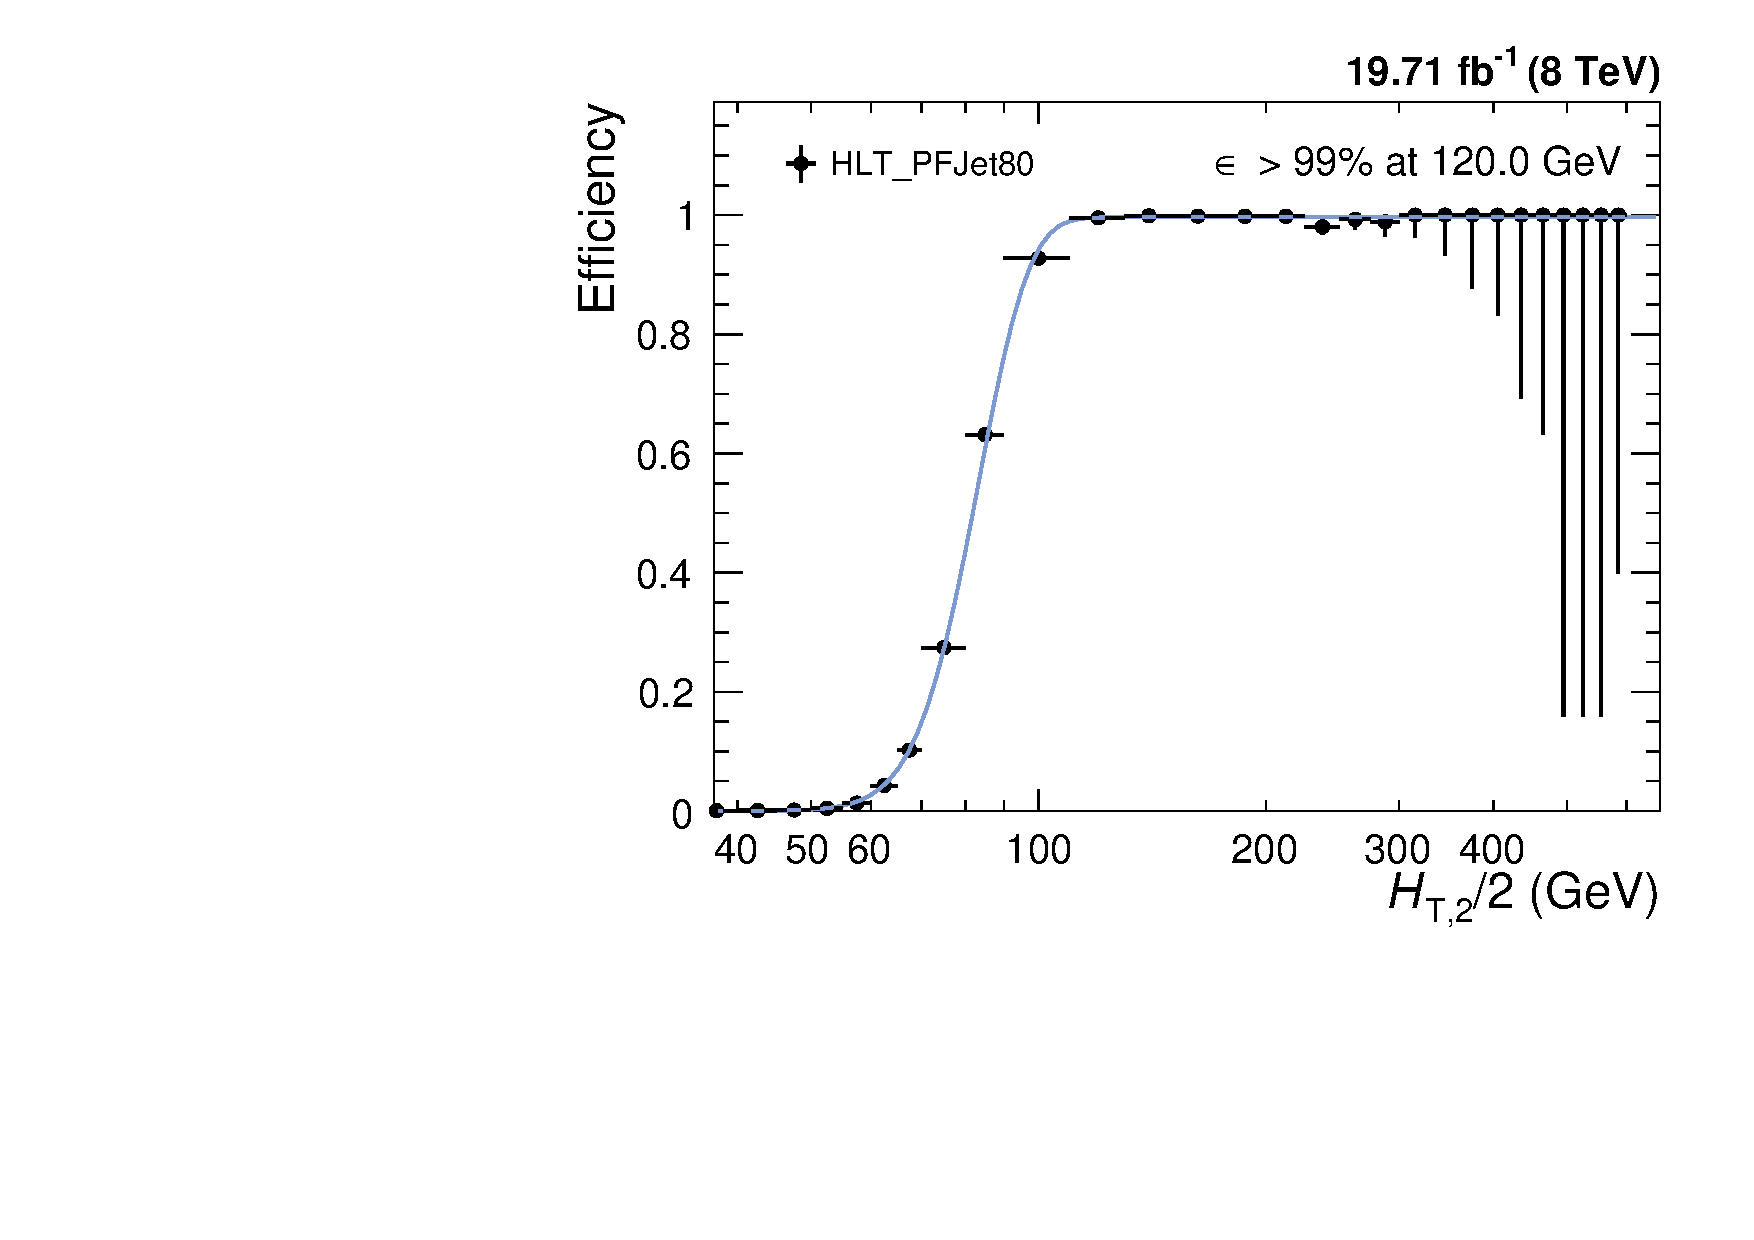
\includegraphics[width=0.5\textwidth]{Plots_HT_2_150/Fit_Turn_Efficiency_80_2_ht_2.pdf}%
    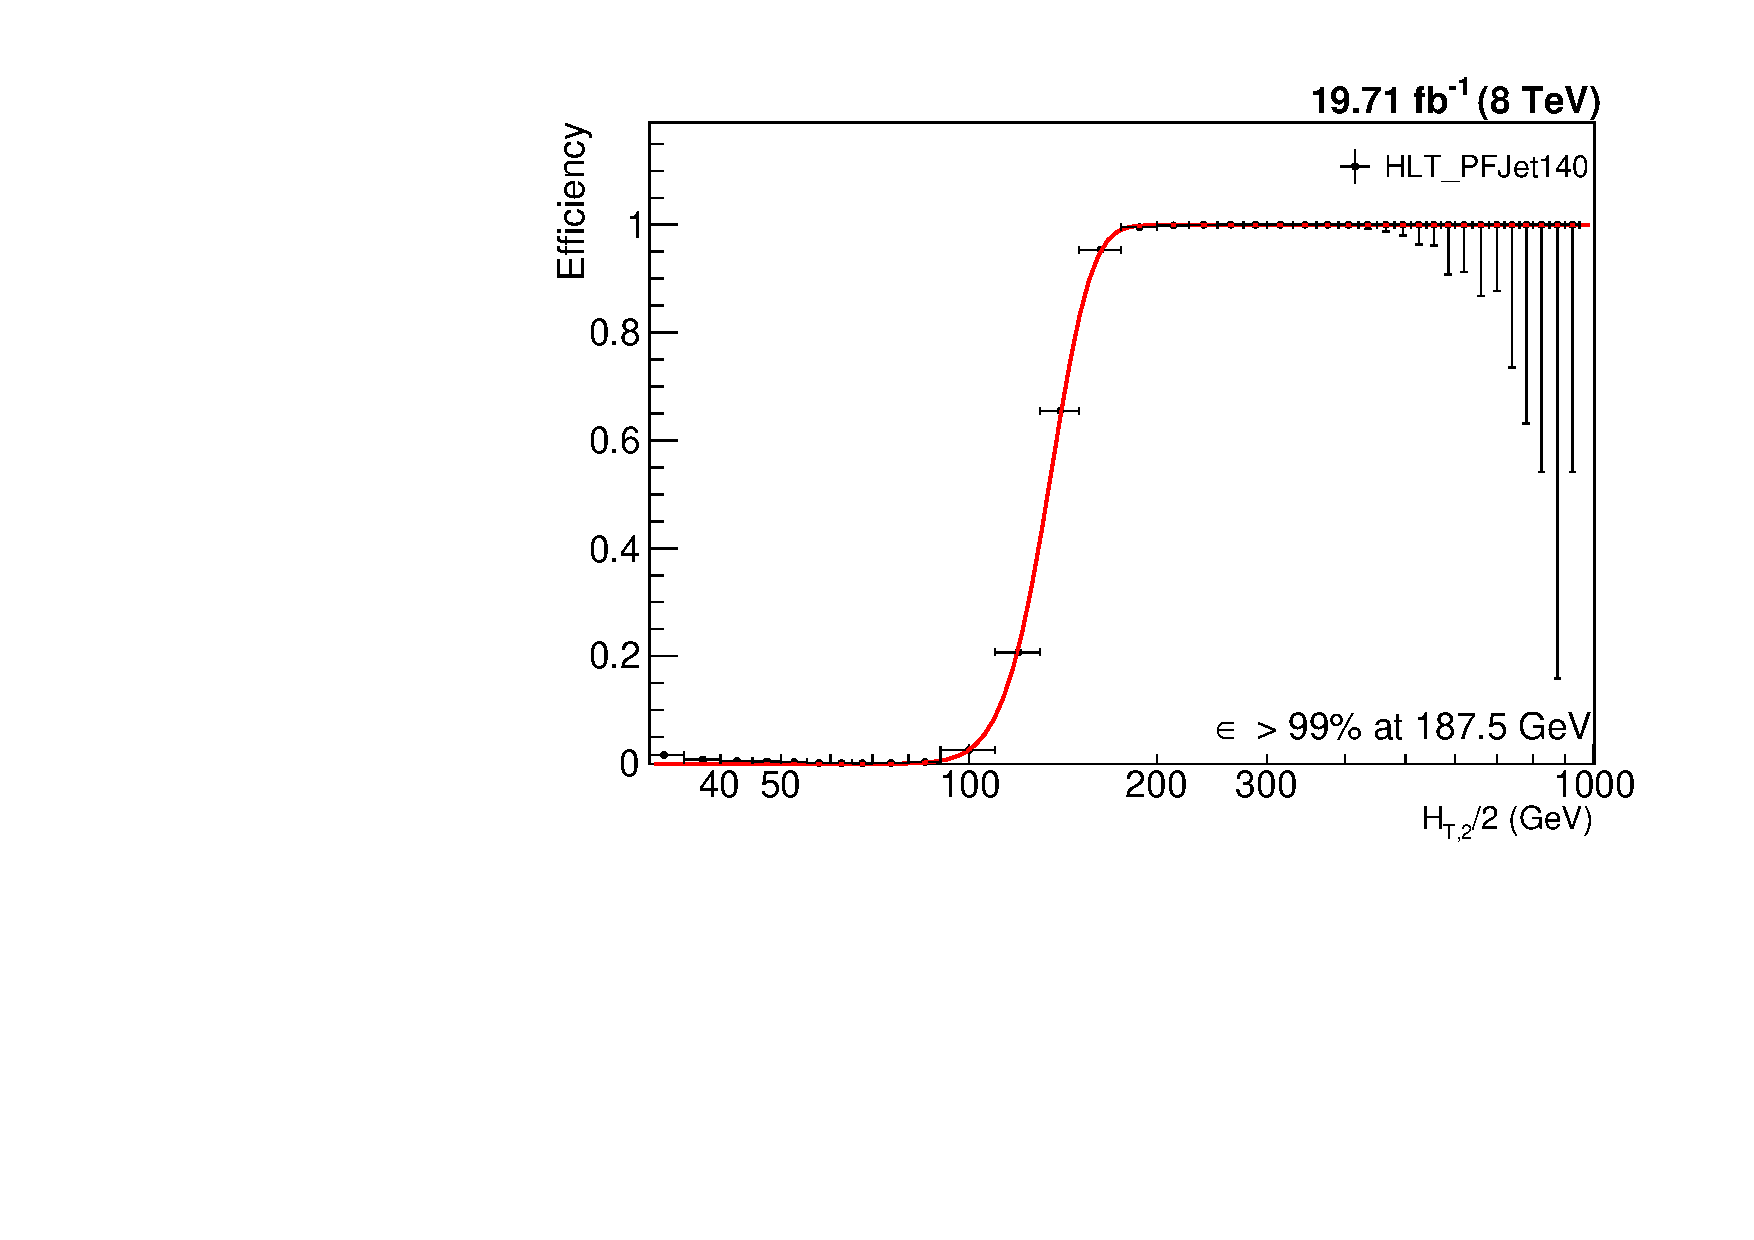
\includegraphics[width=0.5\textwidth]{Plots_HT_2_150/Fit_Turn_Efficiency_140_2_ht_2.pdf}\\
    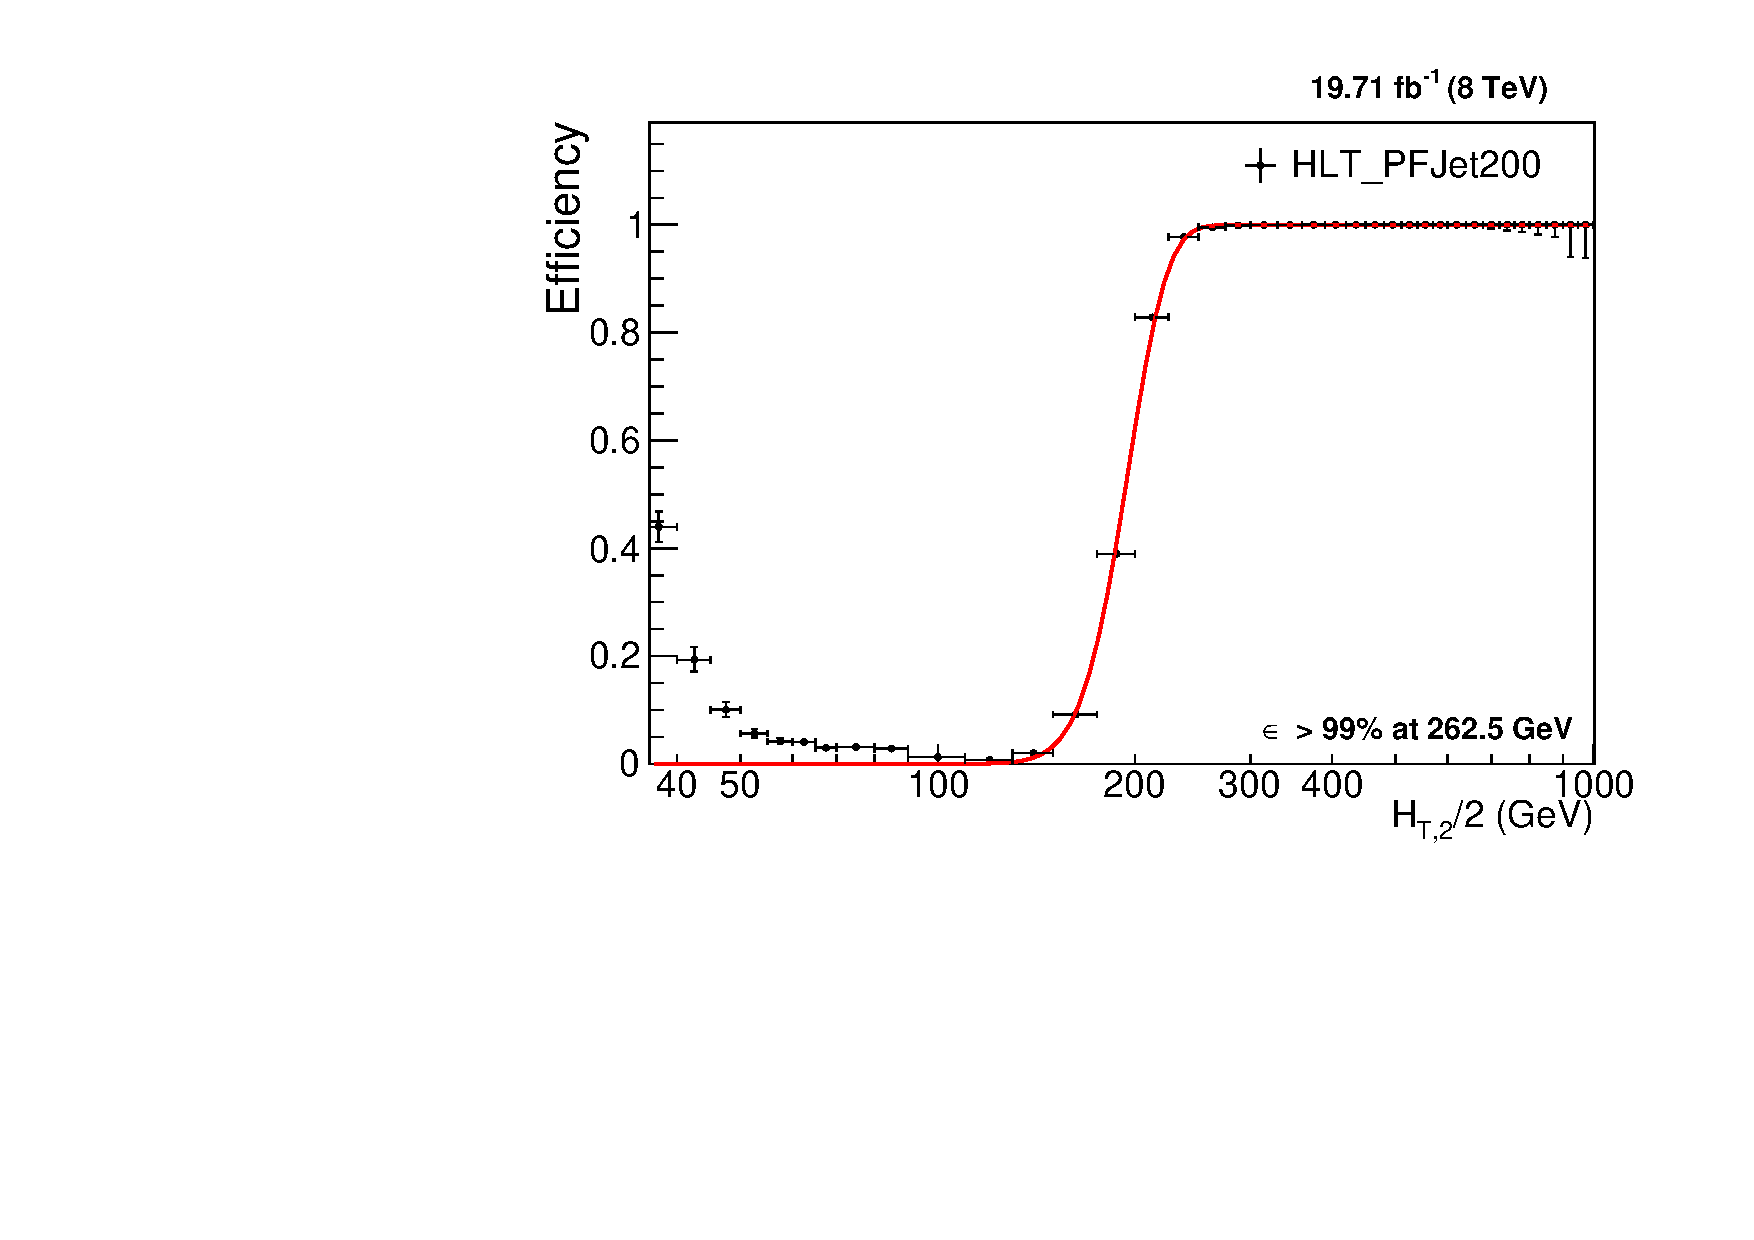
\includegraphics[width=0.5\textwidth]{Plots_HT_2_150/Fit_Turn_Efficiency_200_2_ht_2.pdf}%
    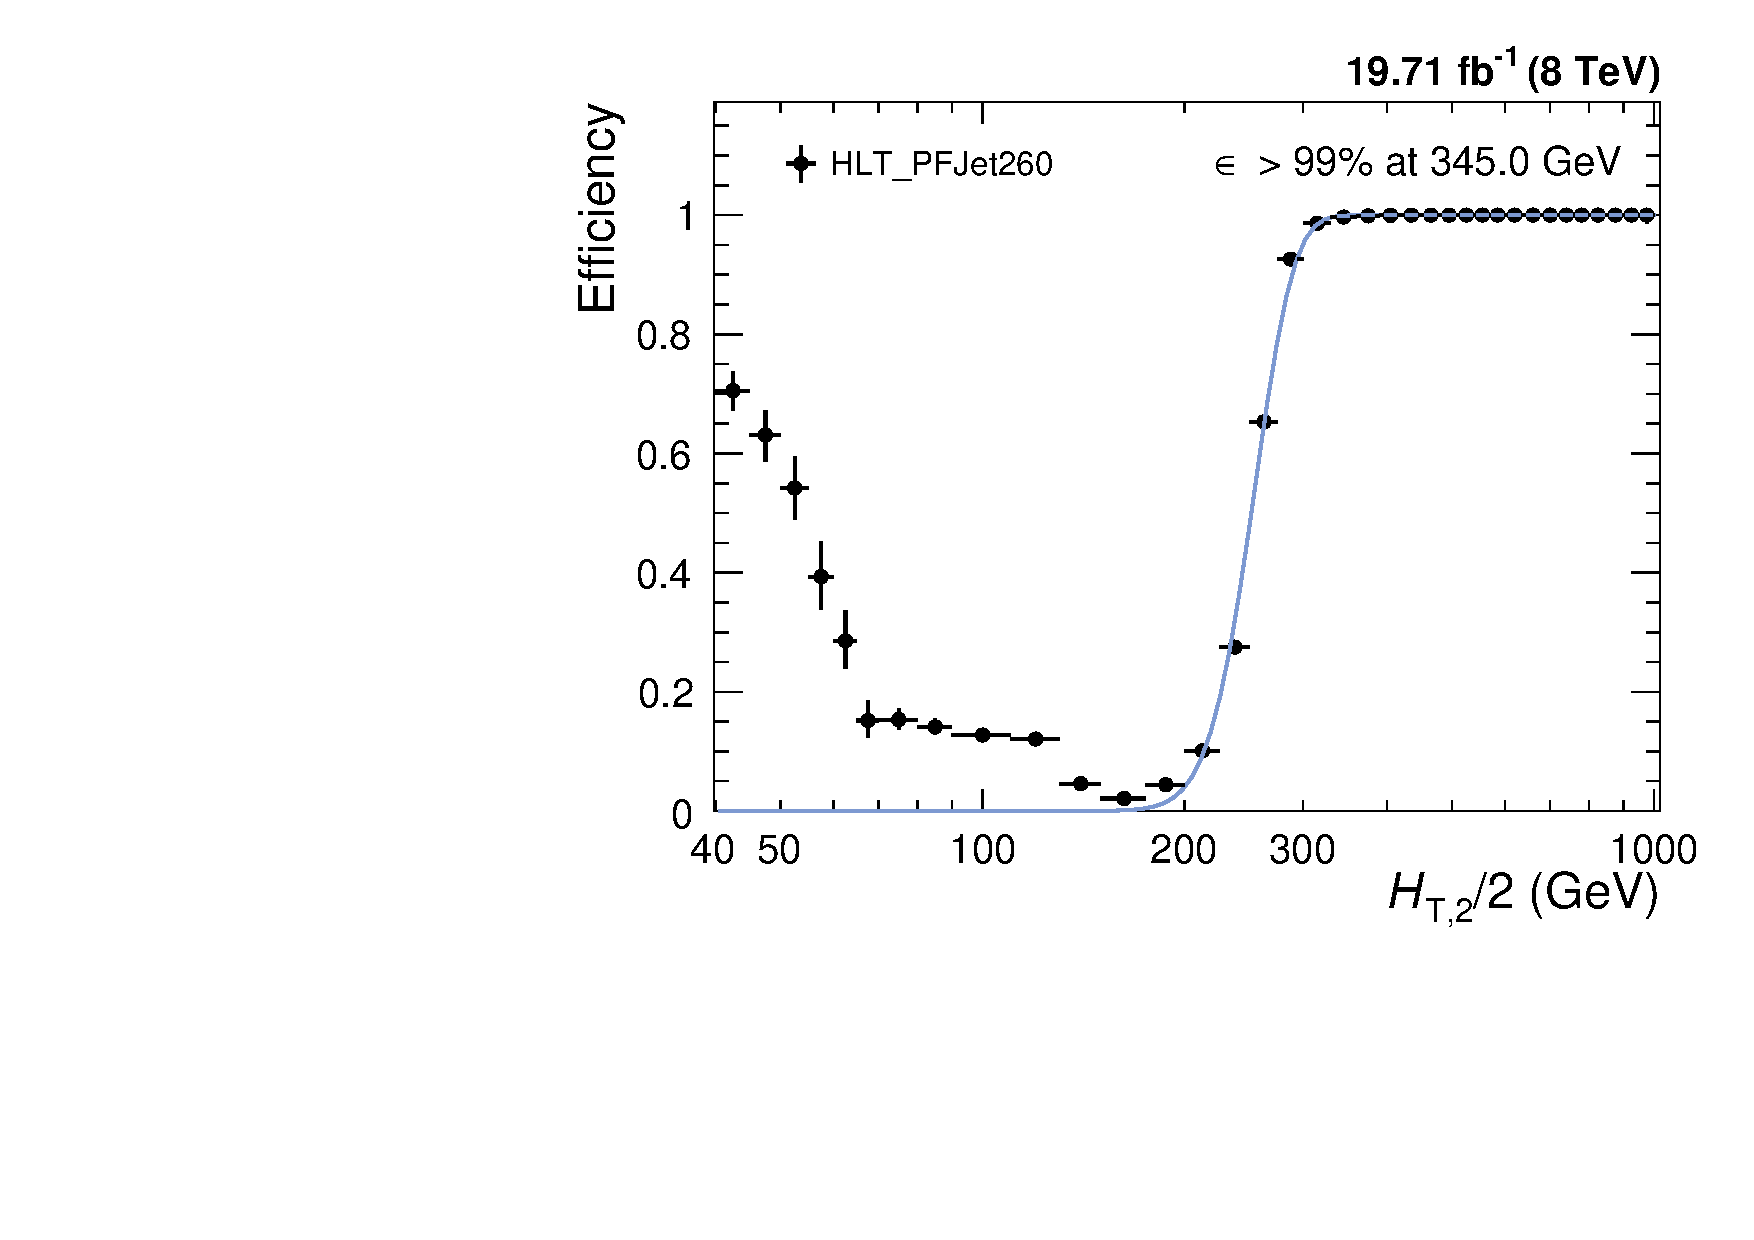
\includegraphics[width=0.5\textwidth]{Plots_HT_2_150/Fit_Turn_Efficiency_260_2_ht_2.pdf}\\
    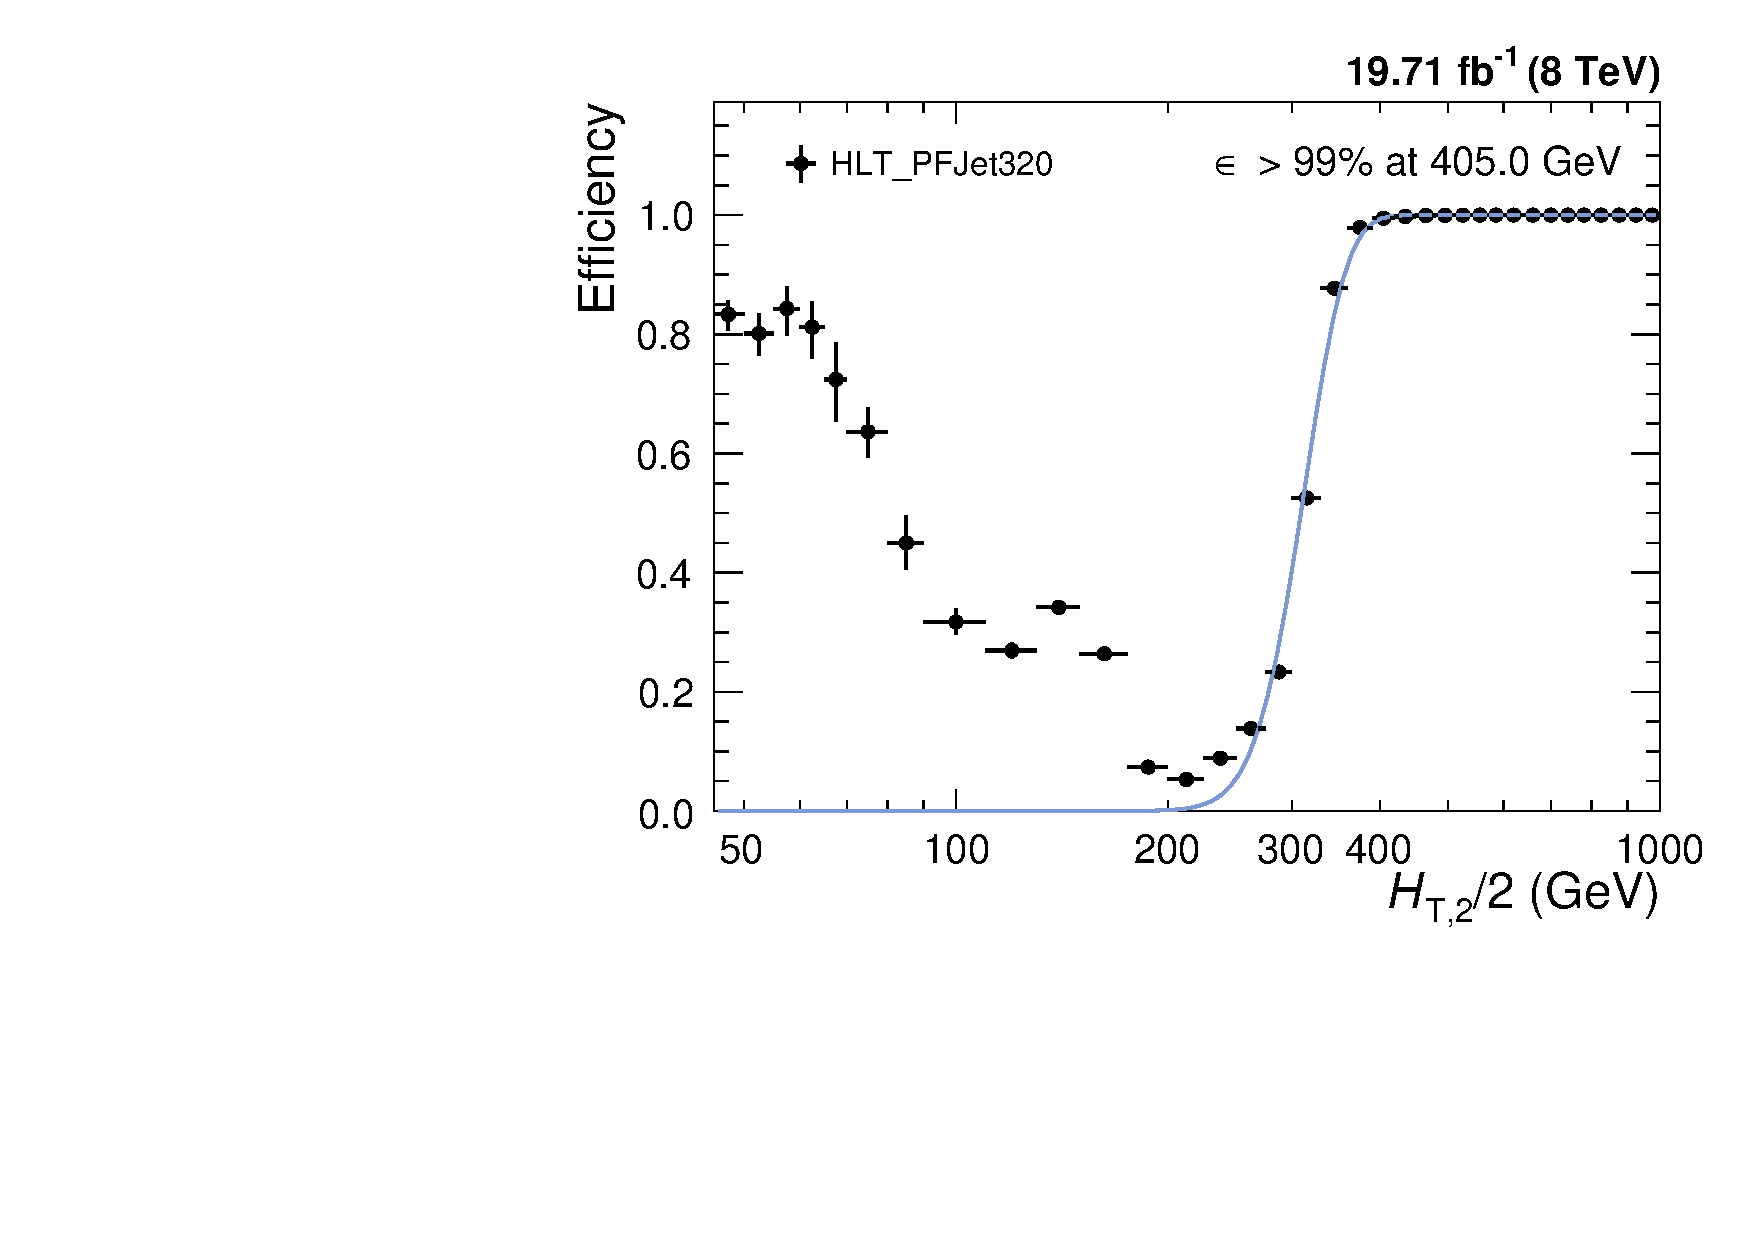
\includegraphics[width=0.5\textwidth]{Plots_HT_2_150/Fit_Turn_Efficiency_320_2_ht_2.pdf}%
    \caption{Trigger efficiencies turn-on curves for the single jet trigger paths used in the analysis.}
    \label{fig:trig_eff}
  \end{center}
\end{figure} 

The trigger efficiency for HLT\_PFJetY is defined as : 

\begin{equation}
  \rm{HLT\_PFJet_{eff}Y = \frac{\httwo (HLT\_PFJetX + L1Object\_\pt > Z + HLTObject\_\pt > Y)}{\httwo (HLT\_PFJetX)}}
\end{equation}

Here the denominator represents the number of events for which the trigger path HLT\_PFJetX has been fired. Here the value of X is chosen 
previous to that of Y in \pt ordering from the trigger list so that the higher trigger condition can be emulated from the lower trigger 
path. The numerator is the number of events for which HLT\_PFJetX has been fired and the \pt of L1Object corresponding to the trigger path 
HLT\_JetX is $\geq$ Z (where Z is the L1 seed value corresponding to the trigger path
HLT\_PFJetY ) and the \pt of HLTObject corresponding to the trigger path HLT JetX is $\geq$ Y. For example, in order to obtain turn on 
curve for HLT\_PFJet260, the immediate HLT path of lower threshold HLT\_PFJet200 is chosen, the \pt cut on L1Object corresponding to the 
trigger path HLT PFJet260 is 128 GeV and \pt cut on HLTObject corresponding to the trigger path
HLT Jet260 is 260 GeV. 
The uncertainty on the efficiency is indicated by error bars which represent Clopper-Pearson confidence intervals.
To determine the point, at which the trigger efficiency is larger than 99\%, the turn-on distribution is fitted using a sigmoid function, 
that describes the turn-on behaviour of the trigger paths.

\begin{equation}
  f_{fit} (x) = \frac {1}{2} \Big( 1 ~\texttt{+}~ erf \Big(\frac {x - \mu}{\sqrt{2} \sigma} \Big) \Big)
\end{equation}

\subsubsection{Primary vertex selection}
A primary vertex (PV) is identified by a collection of tracks, measured 
in the tracker with a good fit quality between the hits and 
compatible with the beam line. The tracks are clustered according to the z-coordinate of 
their point of closest approach to the beam axis. Each event 
is required to have at least one good primary vertex which is well 
reconstructed within a distance of \abs{z(PV)} $<$ 24 cm to the nominal 
interaction point of the detector.

\begin{itemize}
\item Require the radius in x-y plane of PV to be $rho <$ 2 cm.
\item Require the vertex fit no. of degrees of freedom (ndf) $>$ 4. Thus, at least four tracks must be present in order to perform a valid 
  vertex fit.
\end{itemize}

\subsubsection{Jet Identification}
In order to suppress noise and non-physical jets, jet identification criteria (ID) has been applied. The official tight jet ID has been used which are based on the number of constituents inside the reconstructed jets. Instead of applying it event-wise, it 
is applied it on each jet and the following cuts need to be fulfilled by the jets :

\begin{itemize}
\item Each jet should contain at least two particles, one of which should be a charged hadron.
\item The fraction of neutral hadrons and photons should be $<$ 0.90 to remove HCAL noise and ECAL
  noise, respectively. 
\item Muons that are falsely identified and clustered as jets are removed by requiring the muon fraction $<$ 0.80 
\item Based on information of the tracker, additional selection cuts are enforced in the region $\eta$ $<$ 2.4. Jets clustered from 
  misidentified electrons are removed with the condition on charged electromagnetic fraction to be $<$ 0.90. Also, the fraction of charged 
  hadrons in the jet must be larger than zero. 
\end{itemize}

Finally the event selection is as follows : 

\begin{itemize}
\item All jets having \pt $>$ 150 \GeV and \abs{y} $<$ 5 are selected.
\item Events with at least two jets are selected.
\item The two leading jets should have \abs{y} $<$ 2.5 and further jets are counted only, if they lie within the same central rapidity range of \abs{y} $<$ 2.5.
\item In QCD, pure jet events are balanced in \pt and thus exhibit a low level of missing transverse energy, which predominantly is caused 
  by jet calibration and resolution effects of the detector. Therefore, the ratio of missing transverse energy to the total transverse energy
  $\frac{\ETmiss}{\sum \ET}$, both derived from the whole event information, is required to be less than 0.3 to select well measured
  jet events, as shown in Figure~\ref{fig:metcut}. 
\end{itemize}

\begin{figure}[!htbp]
  \begin{center}
    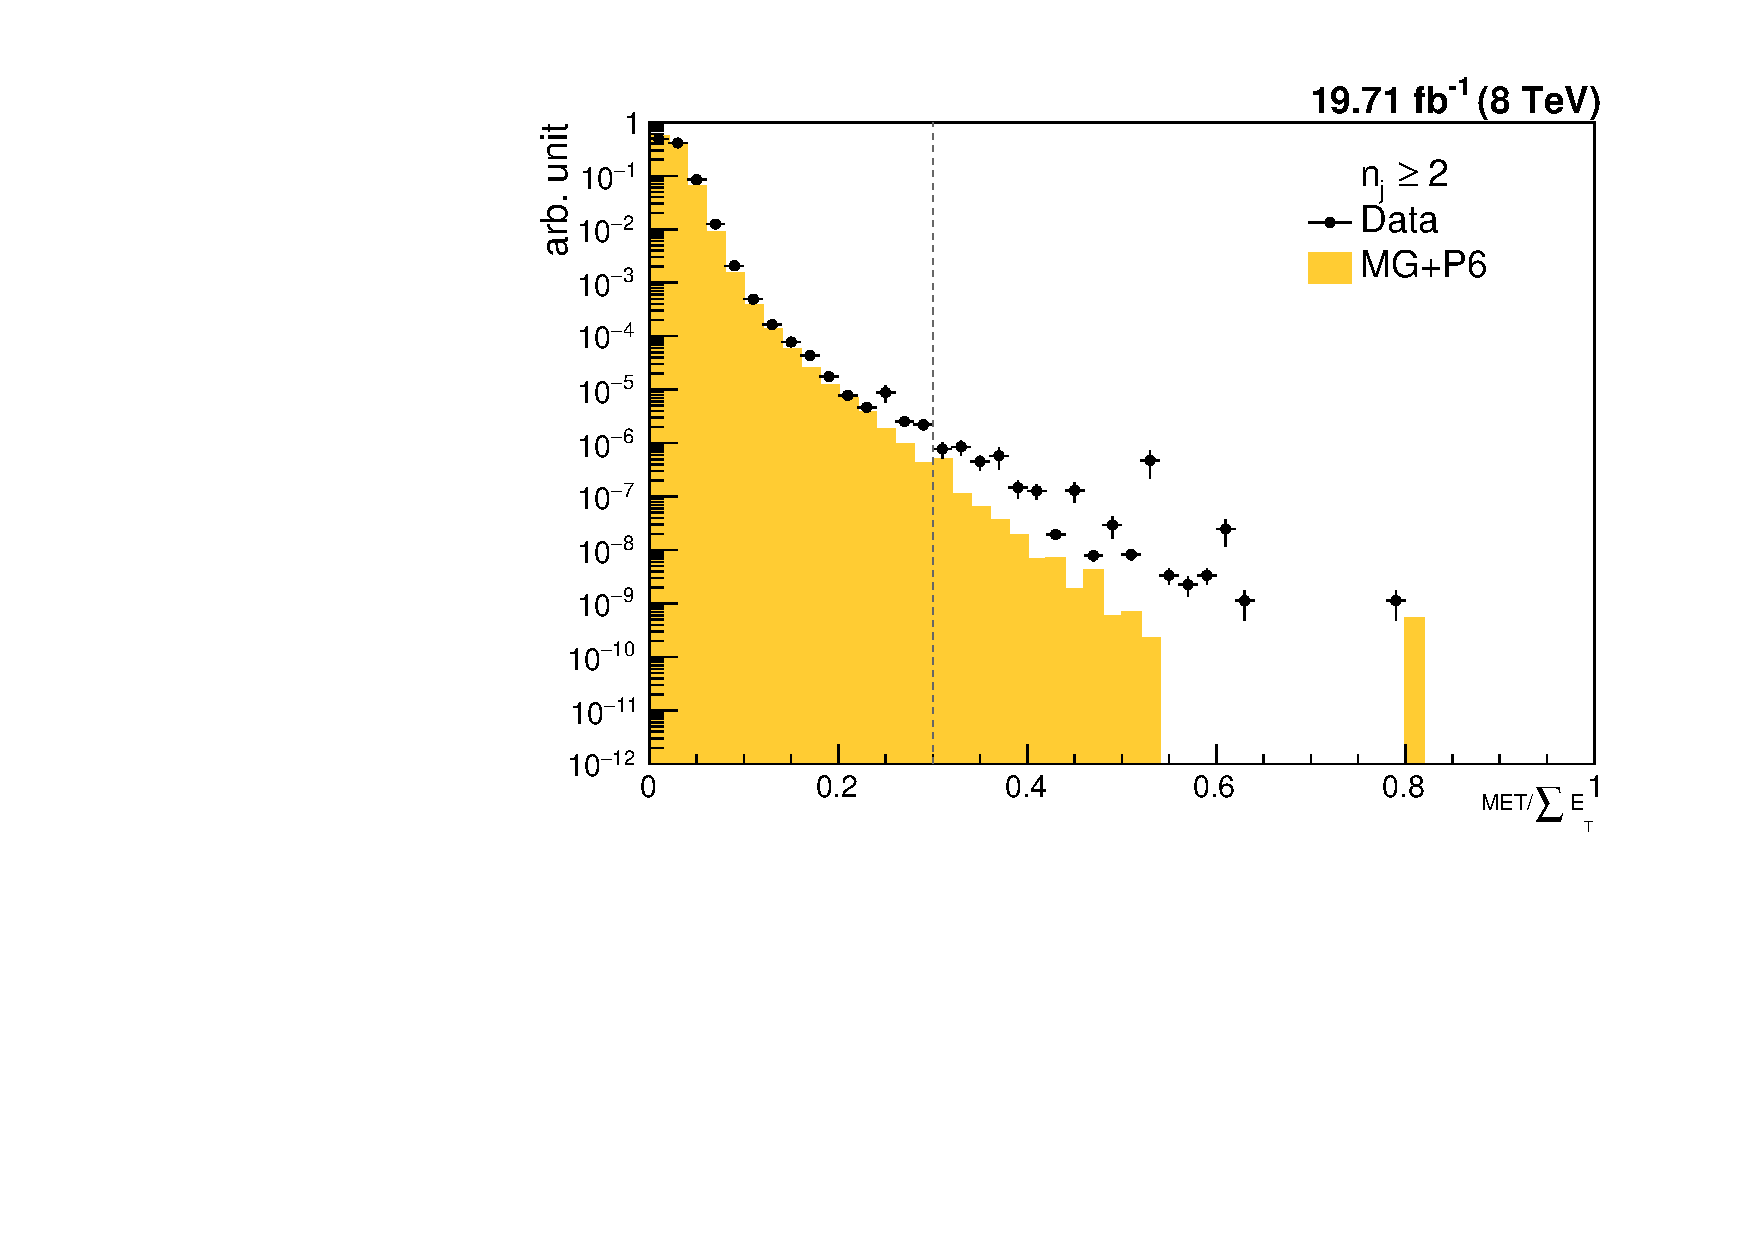
\includegraphics[width=0.5\textwidth]{Plots_HT_2_150/Qual/Missing_ET_2_HT_2_150.pdf}\\
    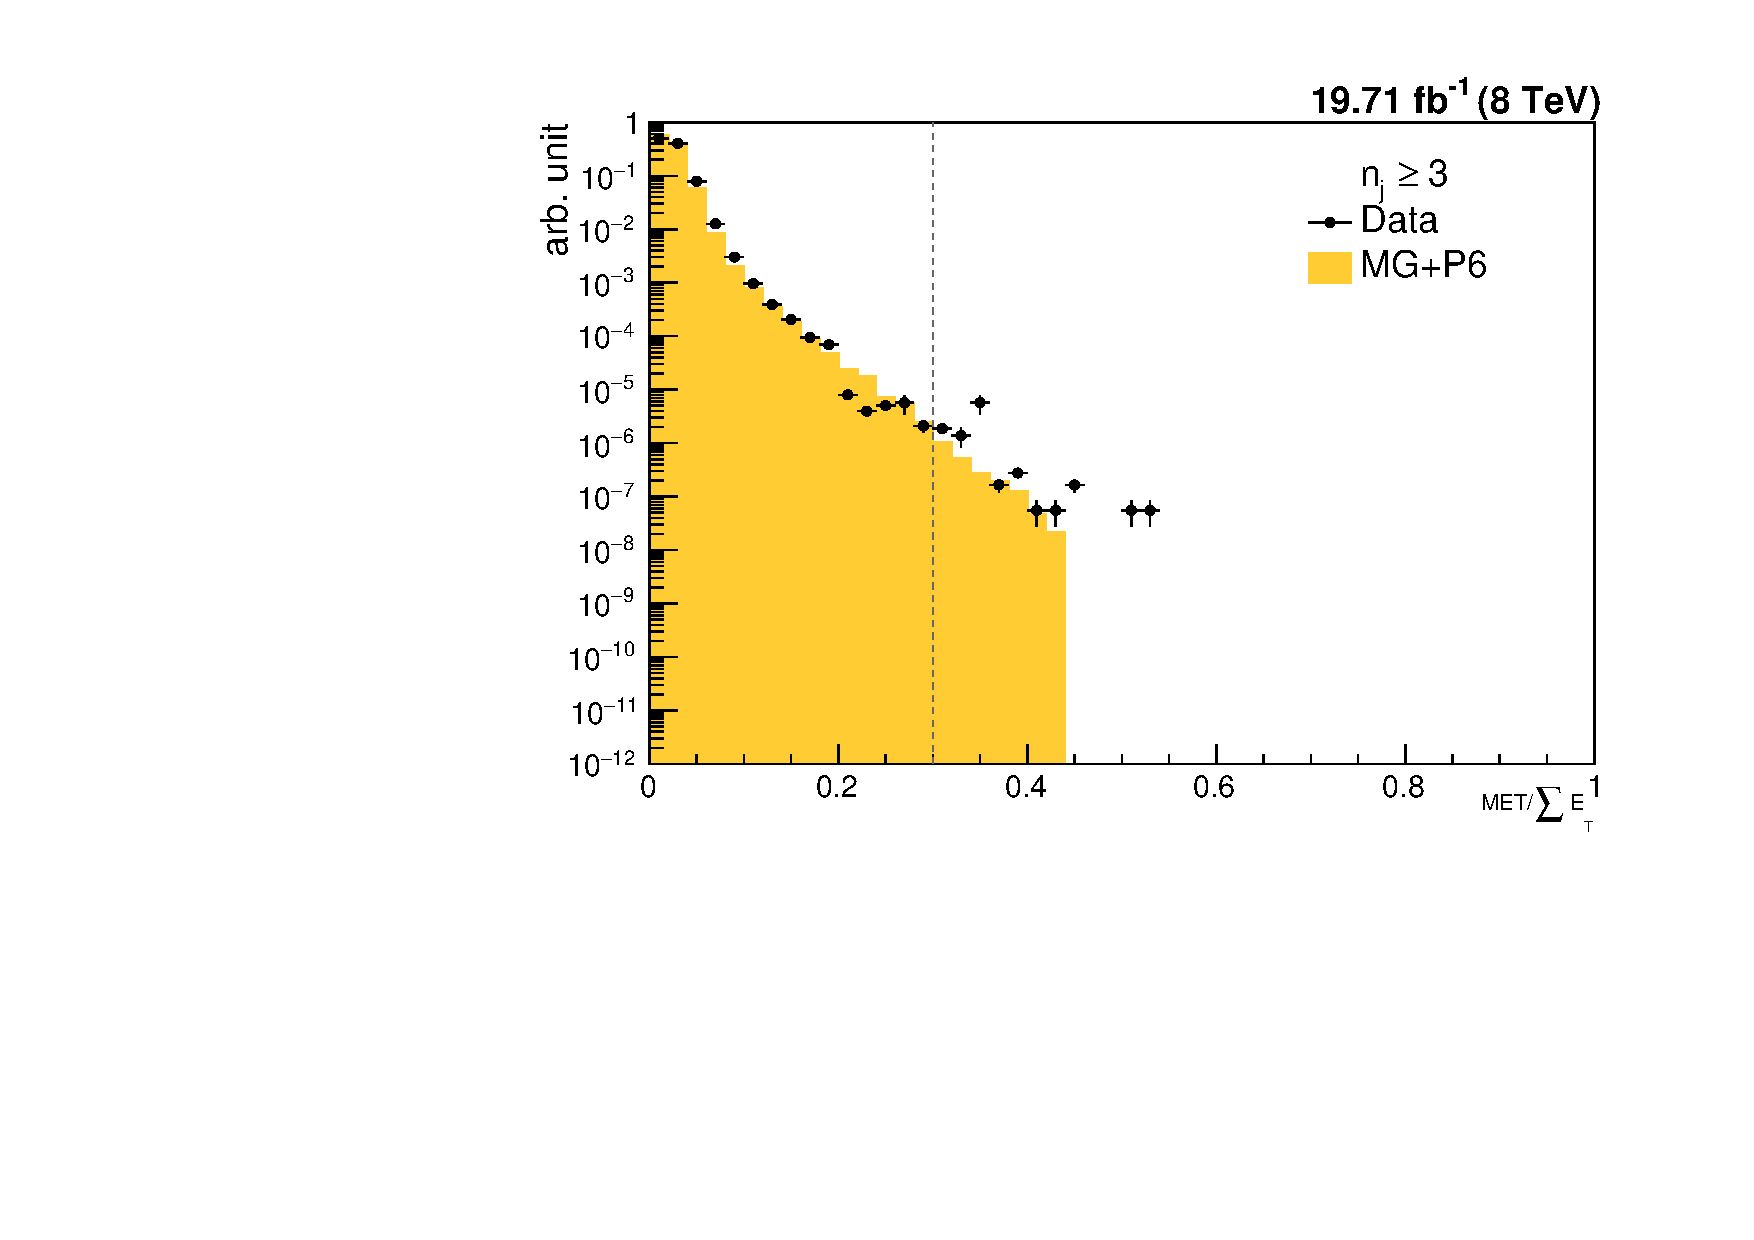
\includegraphics[width=0.5\textwidth]{Plots_HT_2_150/Qual/Missing_ET_3_HT_2_150.pdf}%
    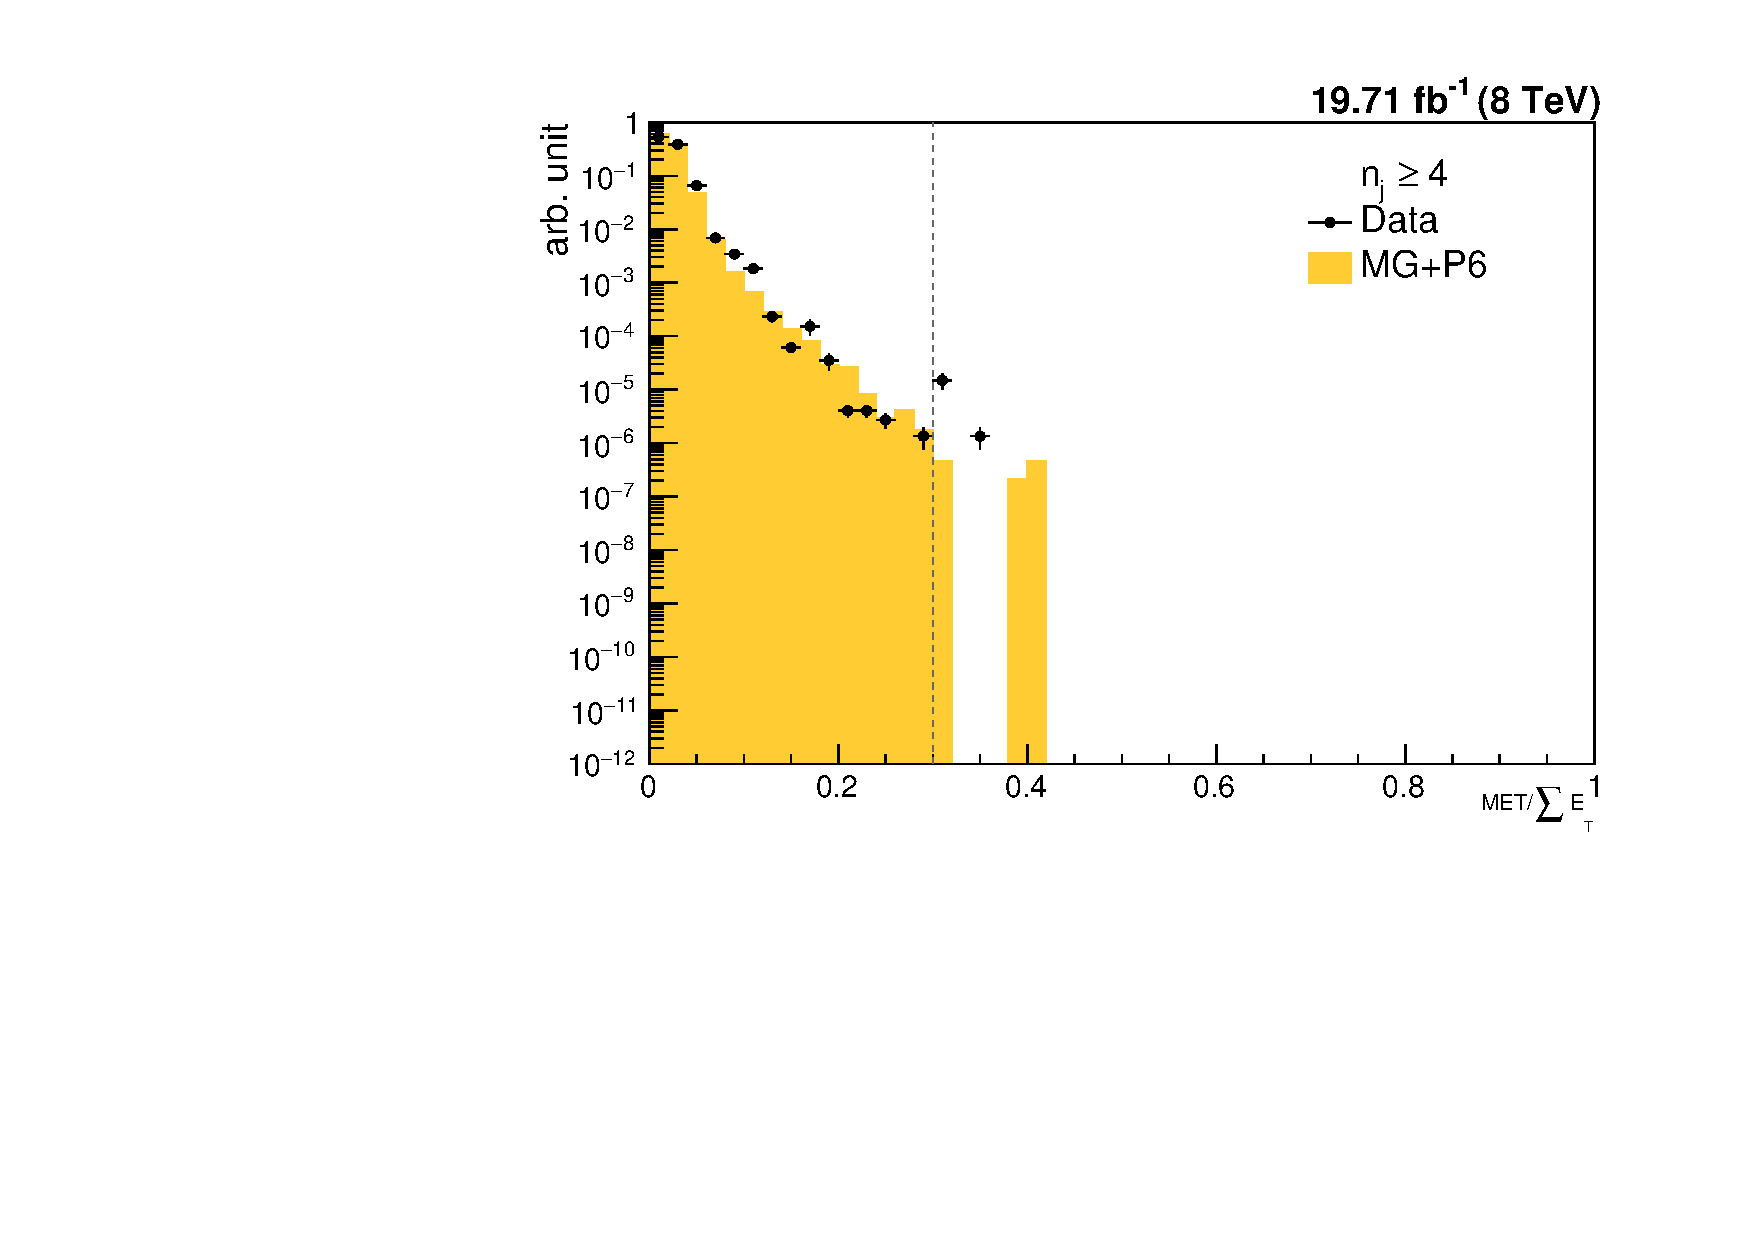
\includegraphics[width=0.5\textwidth]{Plots_HT_2_150/Qual/Missing_ET_4_HT_2_150.pdf}\\
    \caption{Missing transverse energy fraction of the total transverse energy per event
      in data and simulated events. To remove background and noise, events with a fraction
      exceeding a certain threshold, here indicated with the dashed line, are rejected.}
    \label{fig:metcut}
  \end{center}
\end{figure} 

The Figures~\ref{fig:qual2}-~\ref{fig:qual4} show the distributions of the jet constituents observed in data and simulated events for 
inclusive 2-jet, 3-jet and 4-jet events respectively.

\begin{figure}[!htbp]
  \begin{center}
    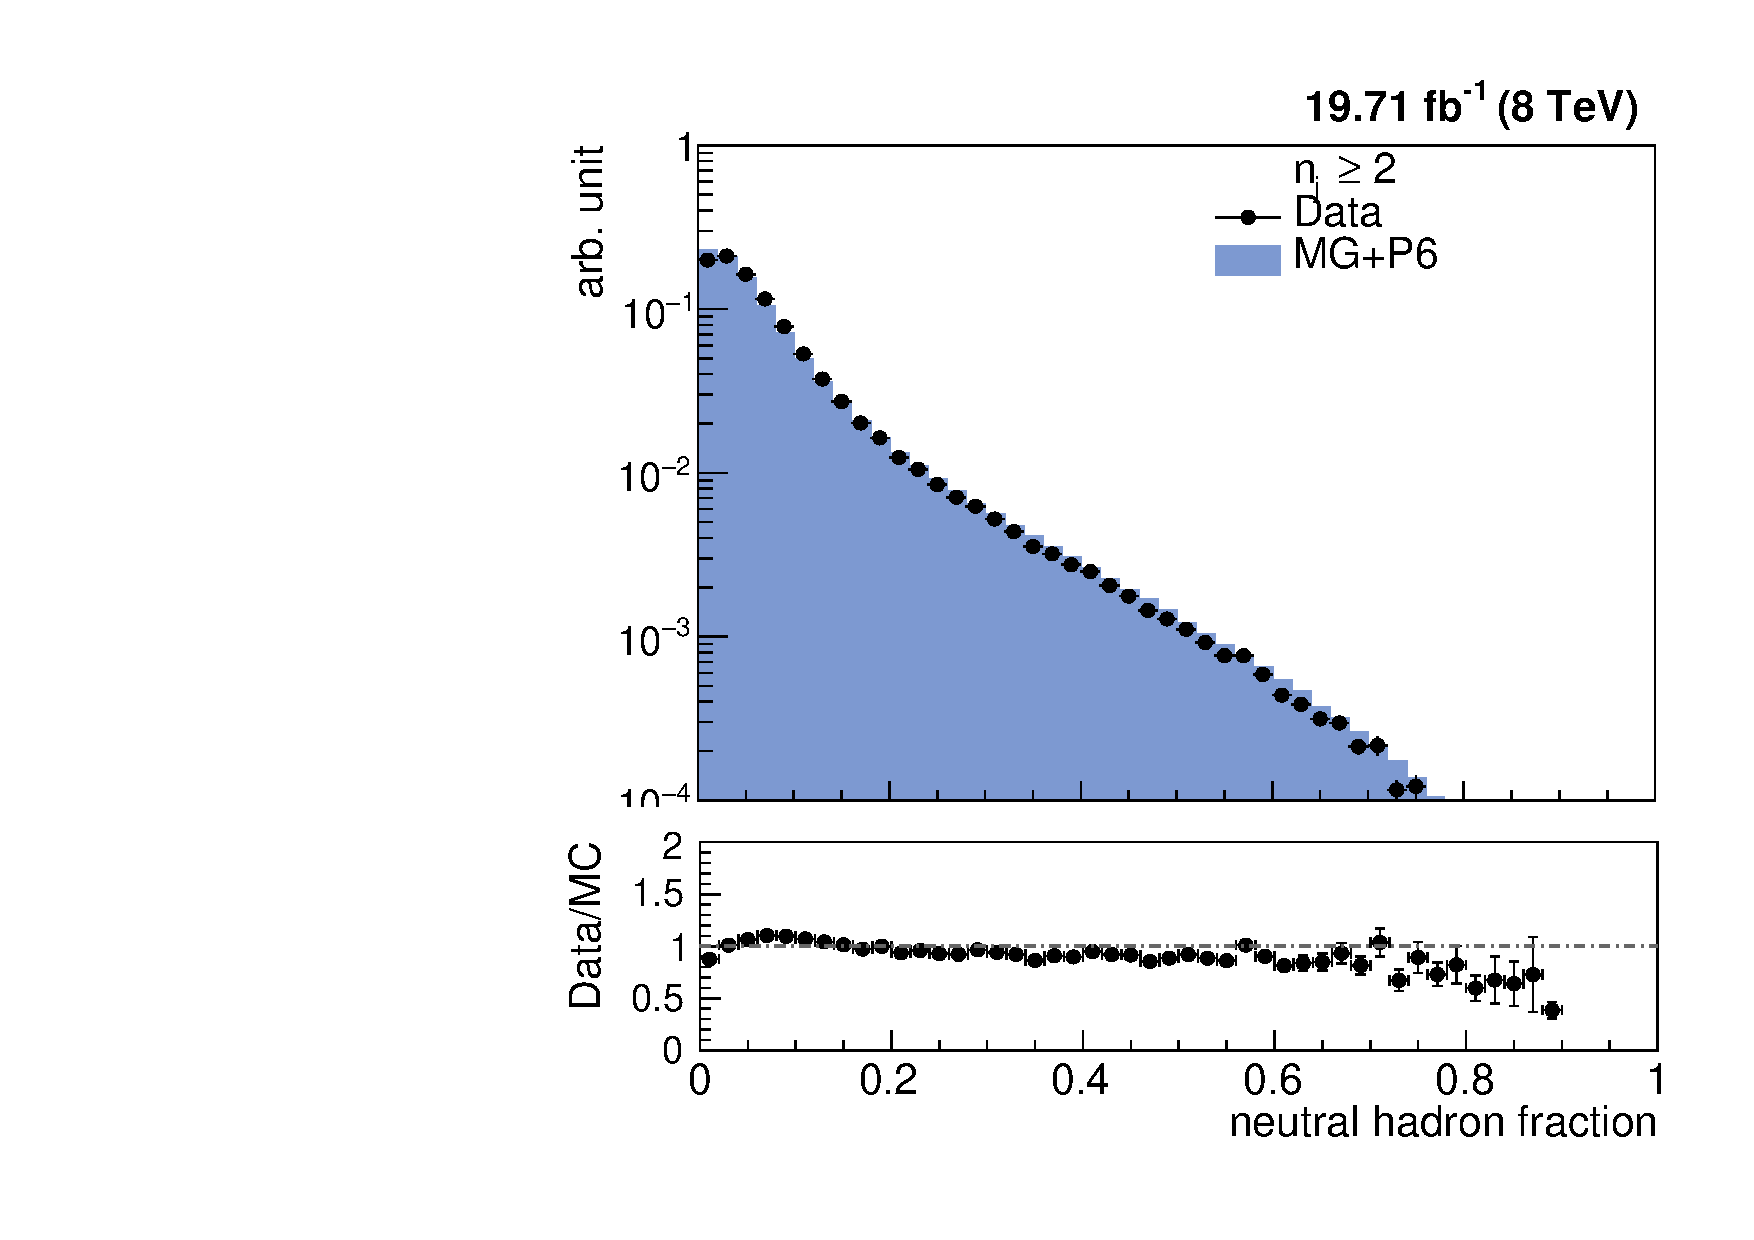
\includegraphics[width=0.5\textwidth]{Plots_HT_2_150/Qual/Comparison_NuHadFrac_2_HT_2_150.pdf}%
    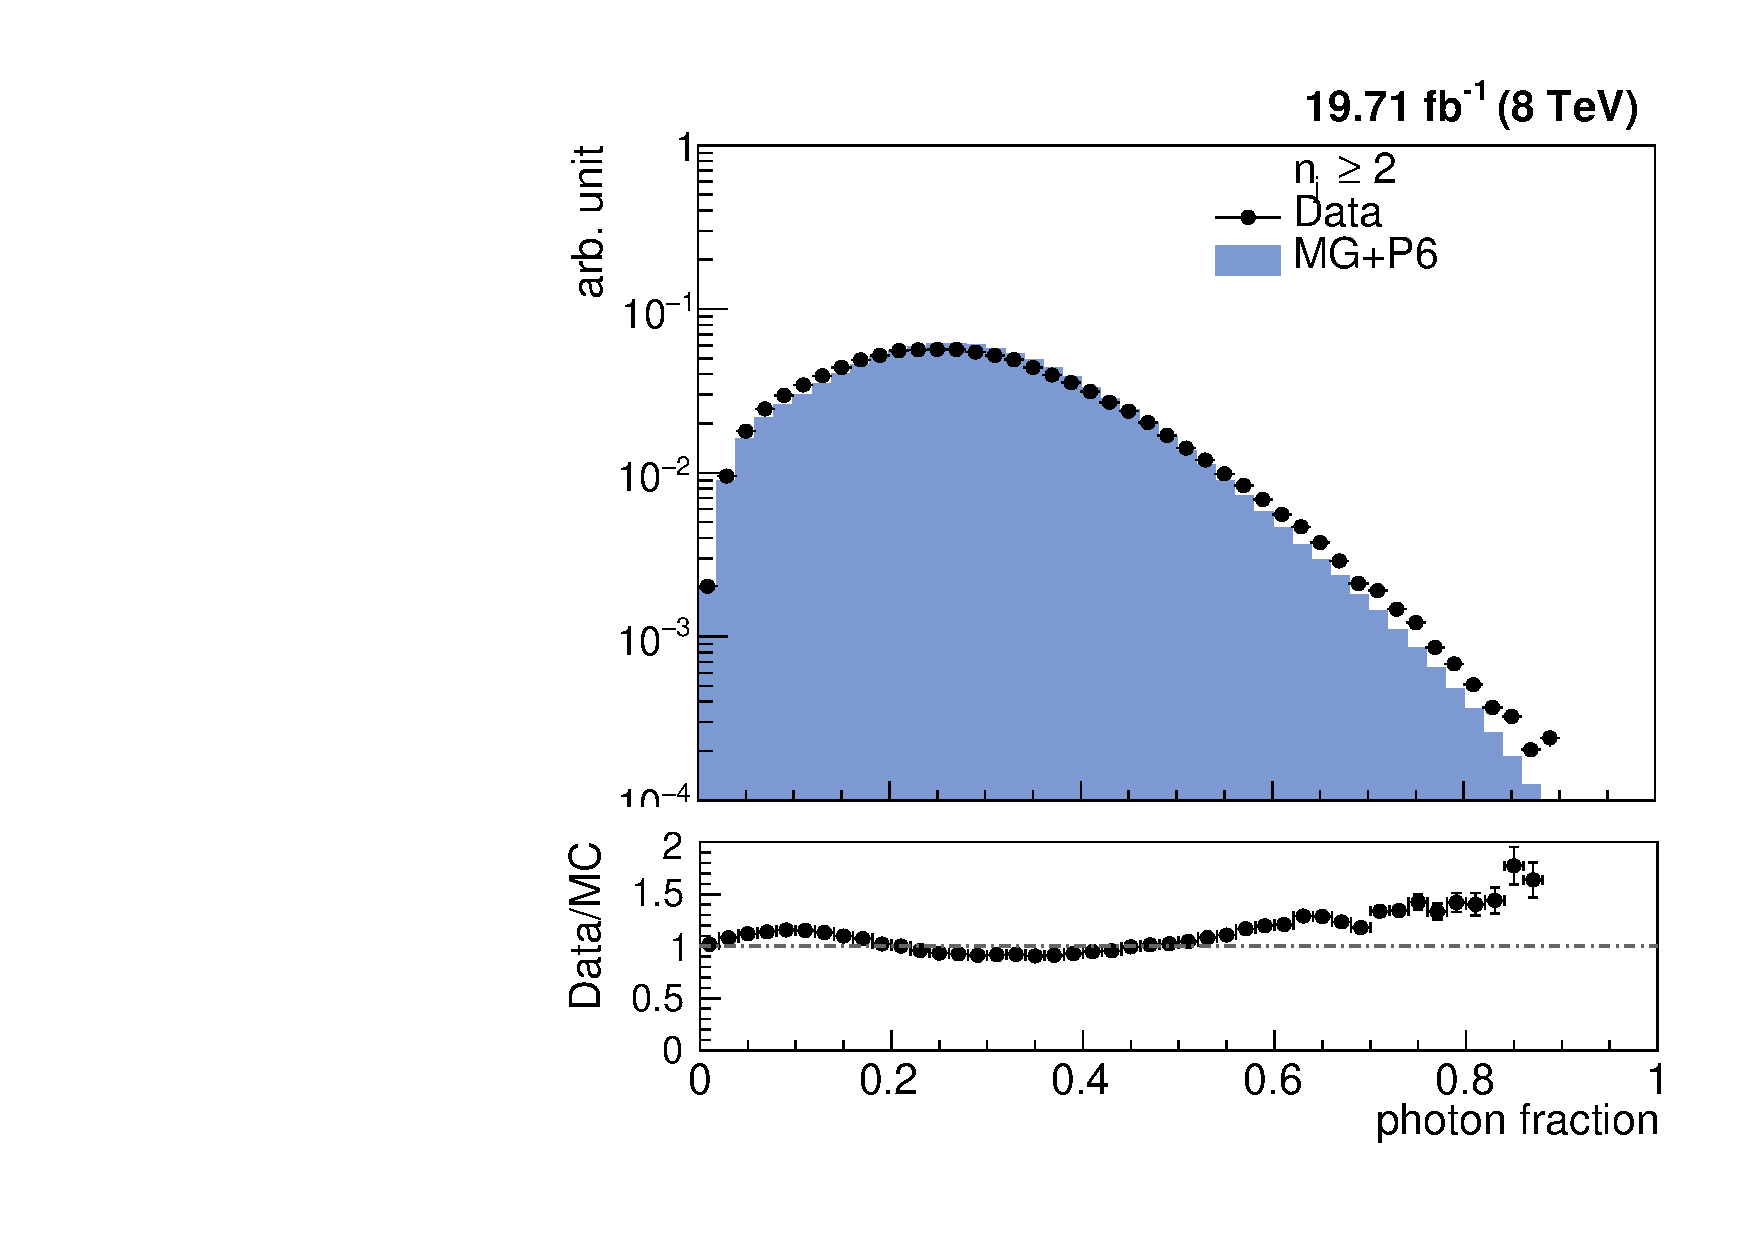
\includegraphics[width=0.5\textwidth]{Plots_HT_2_150/Qual/Comparison_PhFrac_2_HT_2_150.pdf}\\
    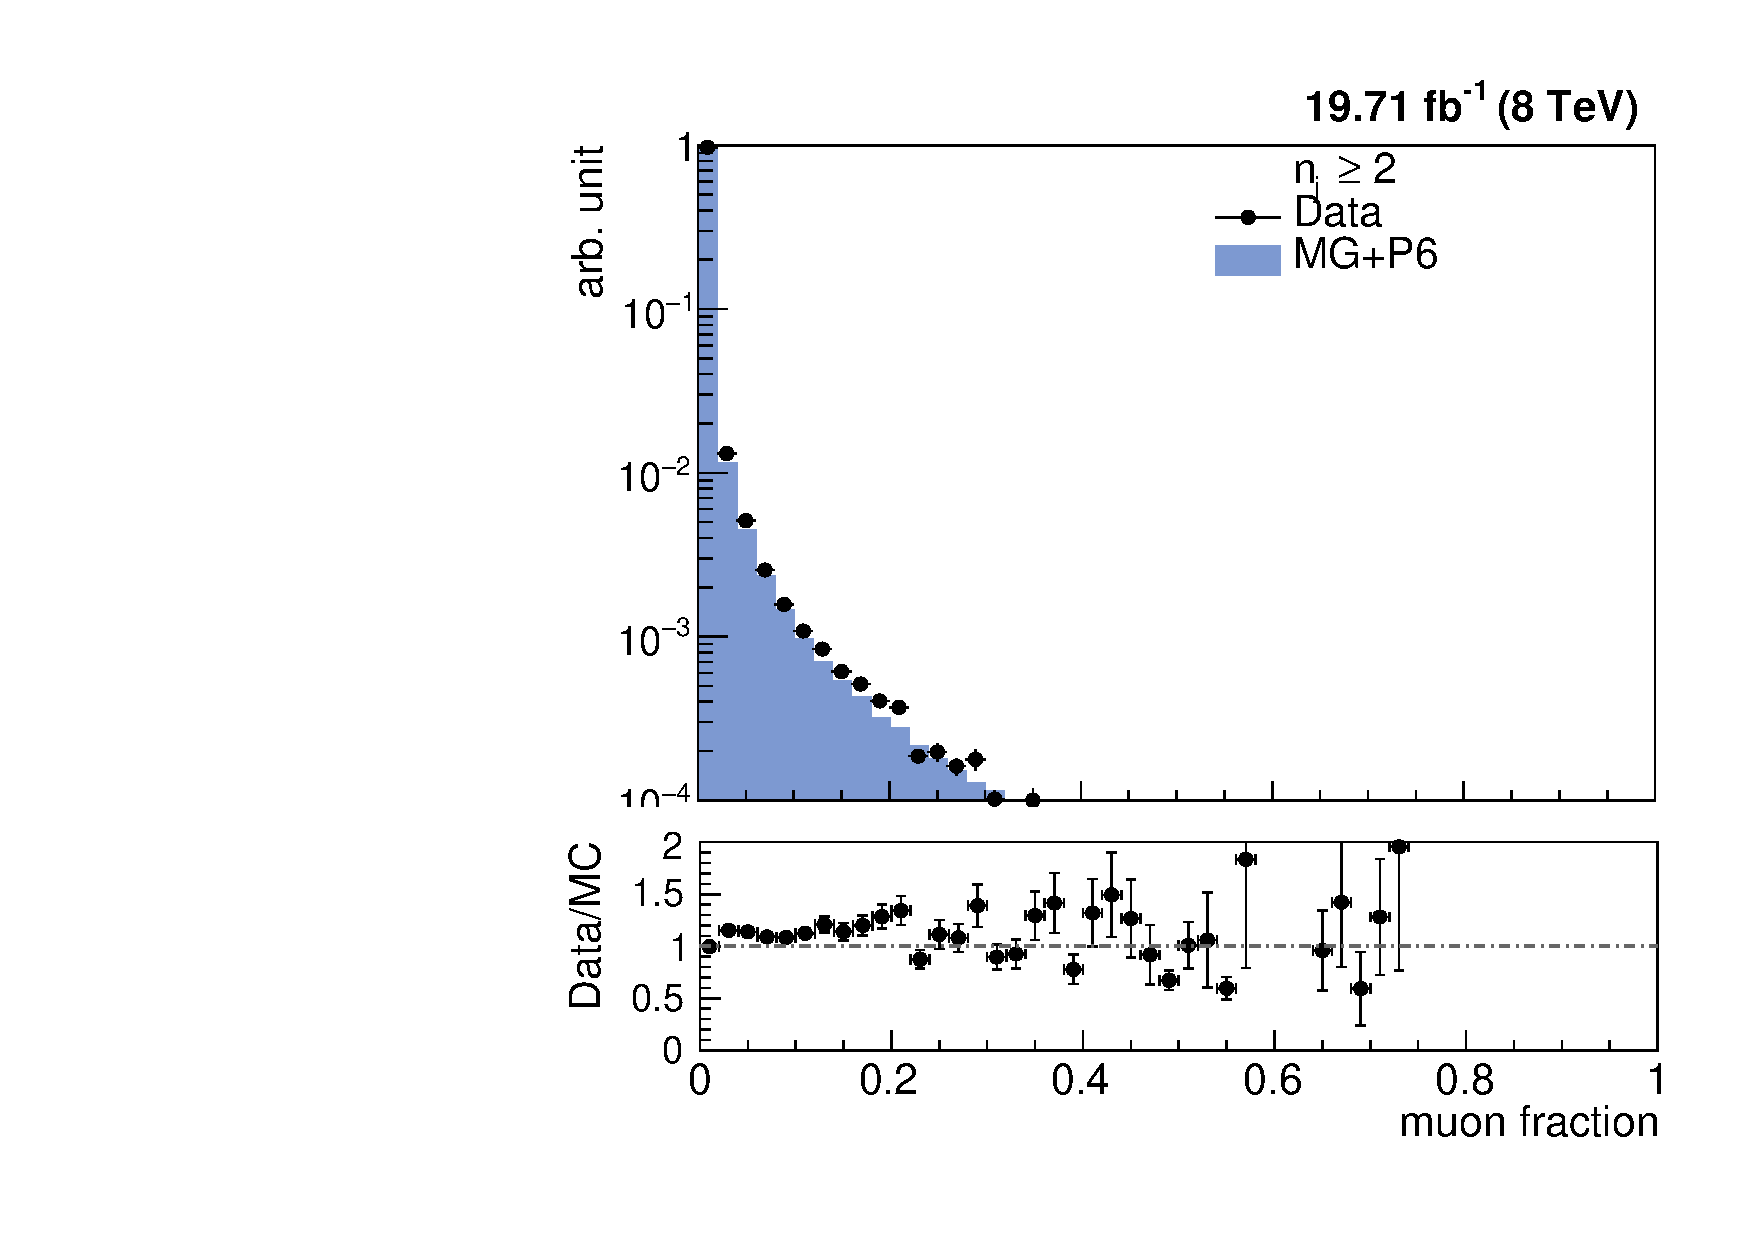
\includegraphics[width=0.5\textwidth]{Plots_HT_2_150/Qual/Comparison_MuFrac_2_HT_2_150.pdf}%
    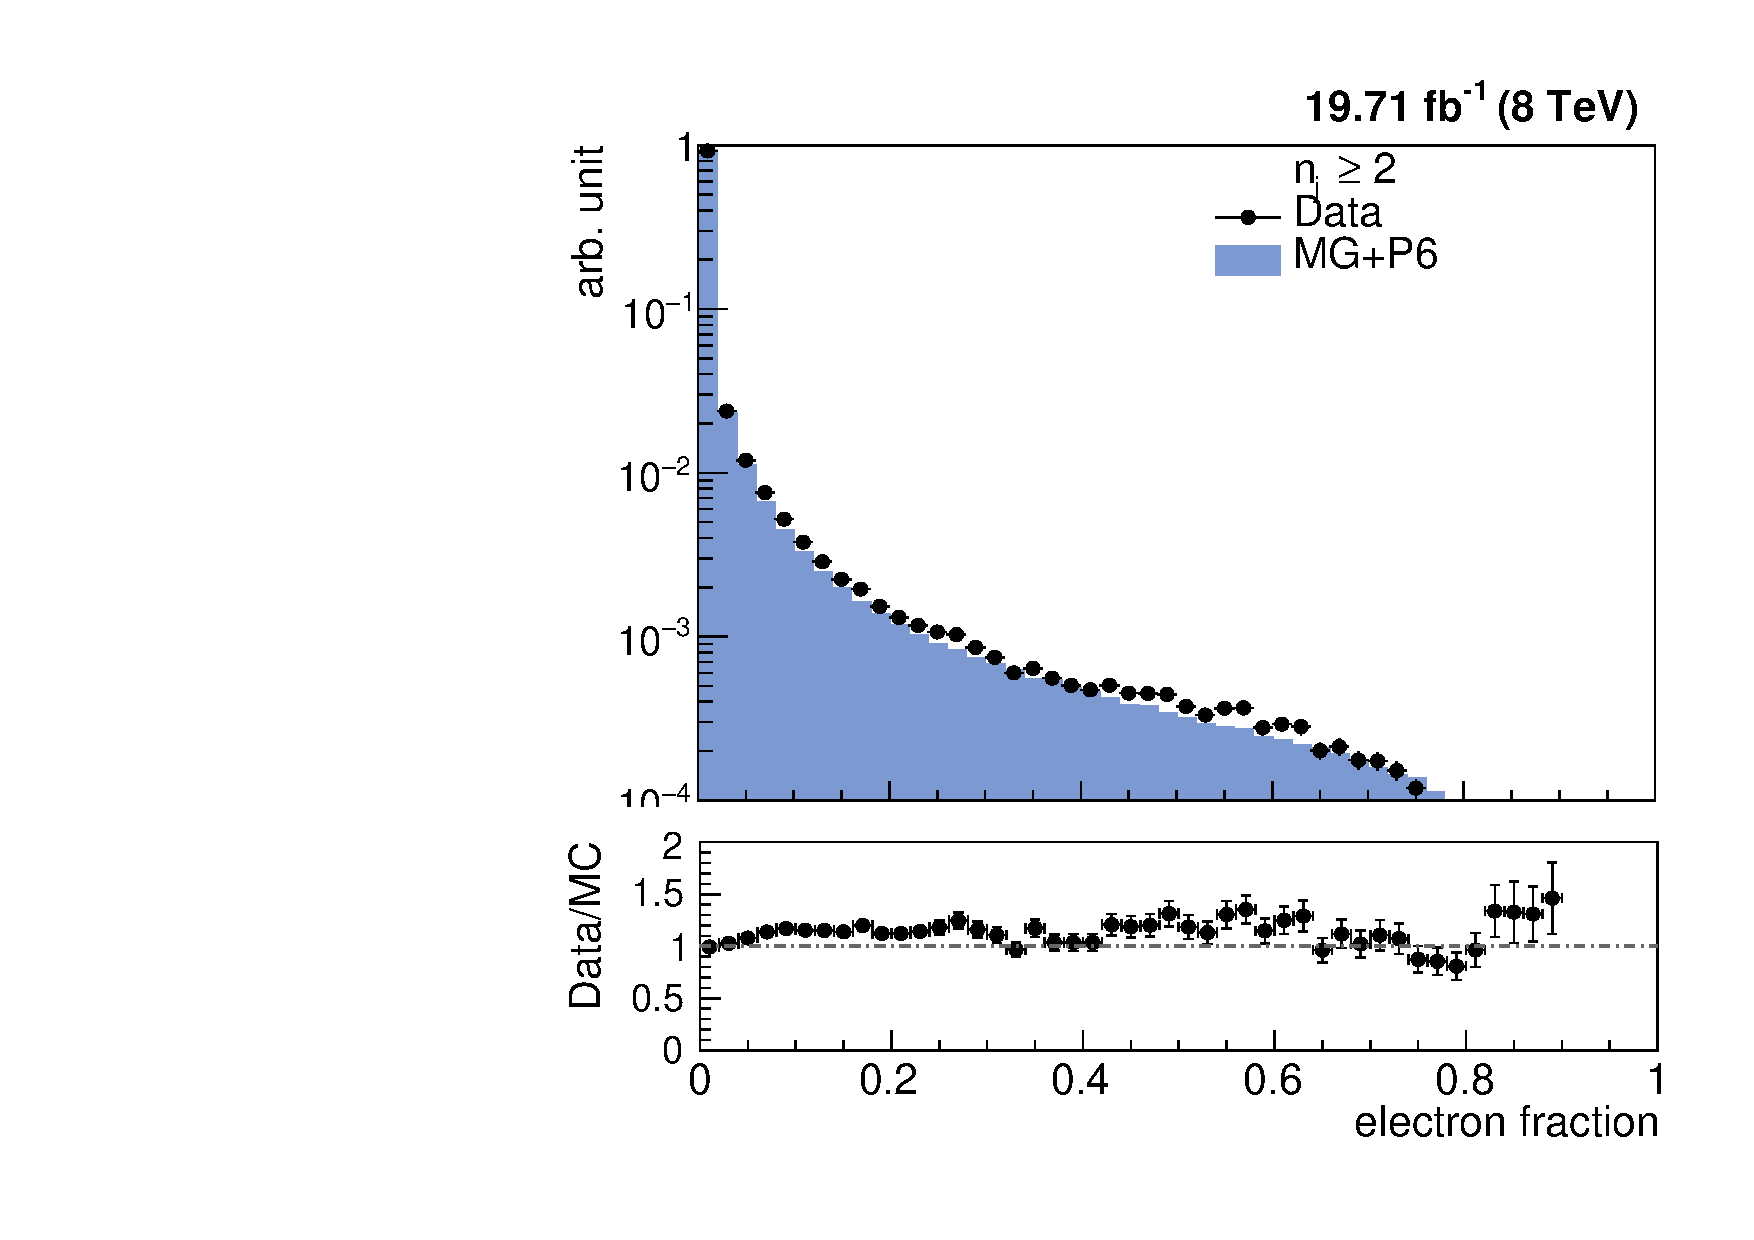
\includegraphics[width=0.5\textwidth]{Plots_HT_2_150/Qual/Comparison_ElFrac_2_HT_2_150.pdf}\\
    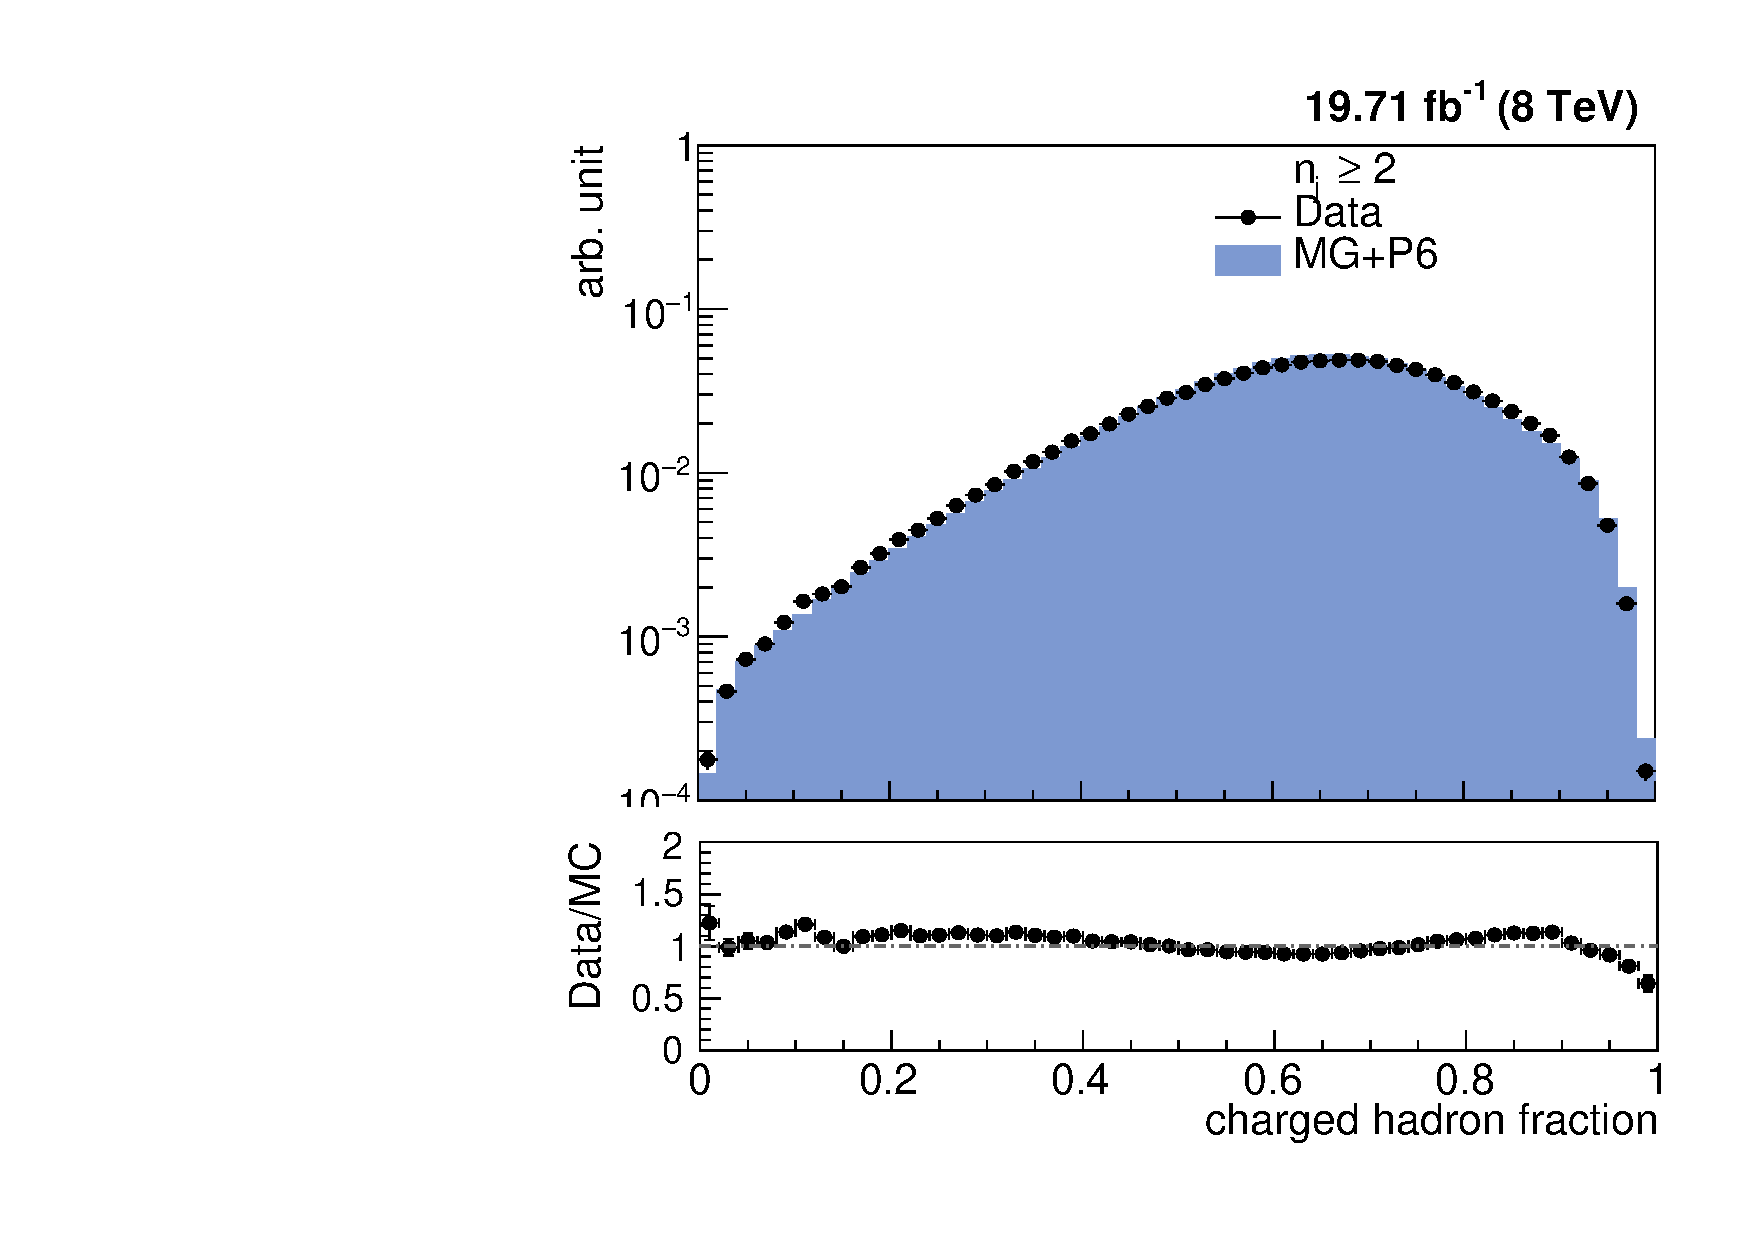
\includegraphics[width=0.5\textwidth]{Plots_HT_2_150/Qual/Comparison_ChHadFrac_2_HT_2_150.pdf}%
    \caption{The fractions of jet constituents as observed in data and simulated events for different types of PF candidates for inclusive 2-jet events. Data and simulation are normalized to the same number of events. The distributions are shown after the application of the jet ID.}
    \label{fig:qual2}
  \end{center}
\end{figure} 

\begin{figure}[!htbp]
  \begin{center}
    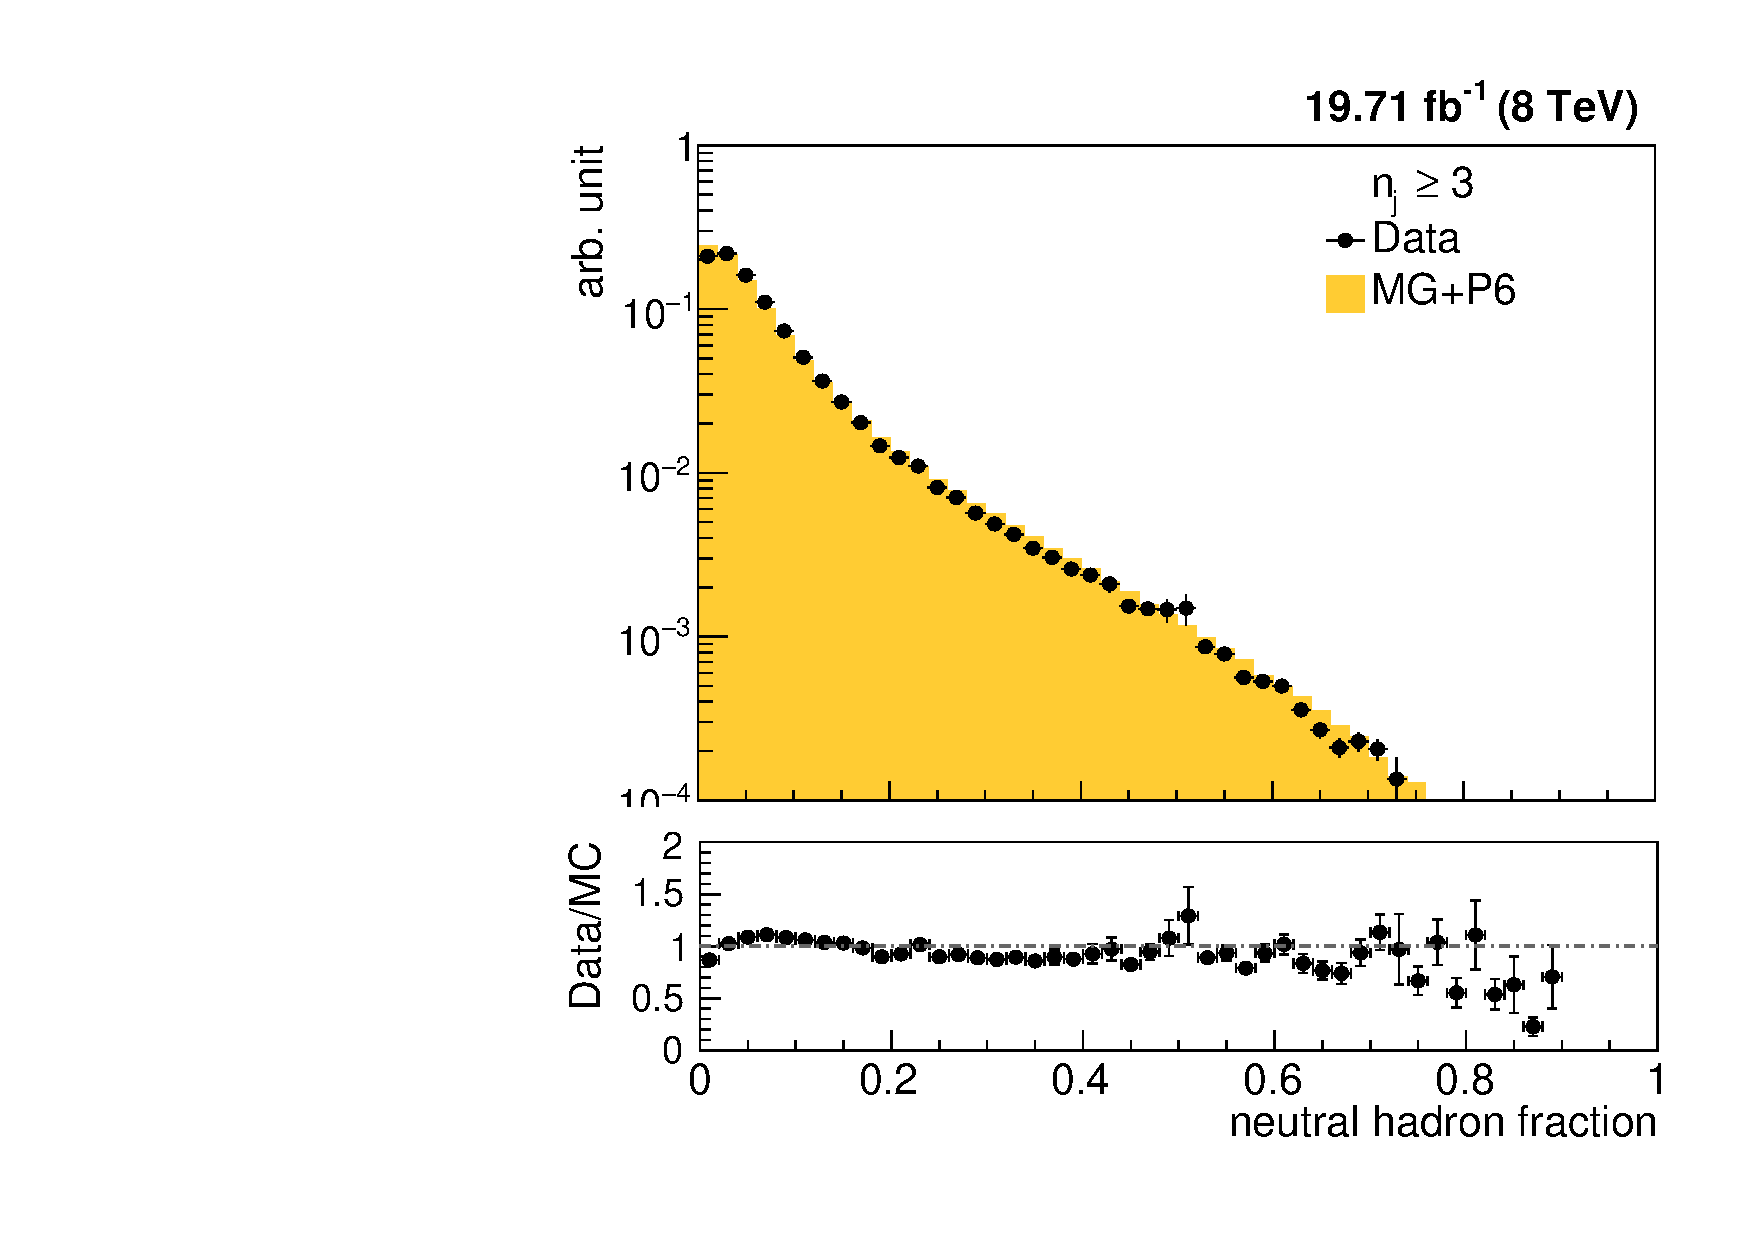
\includegraphics[width=0.5\textwidth]{Plots_HT_2_150/Qual/Comparison_NuHadFrac_3_HT_2_150.pdf}%
    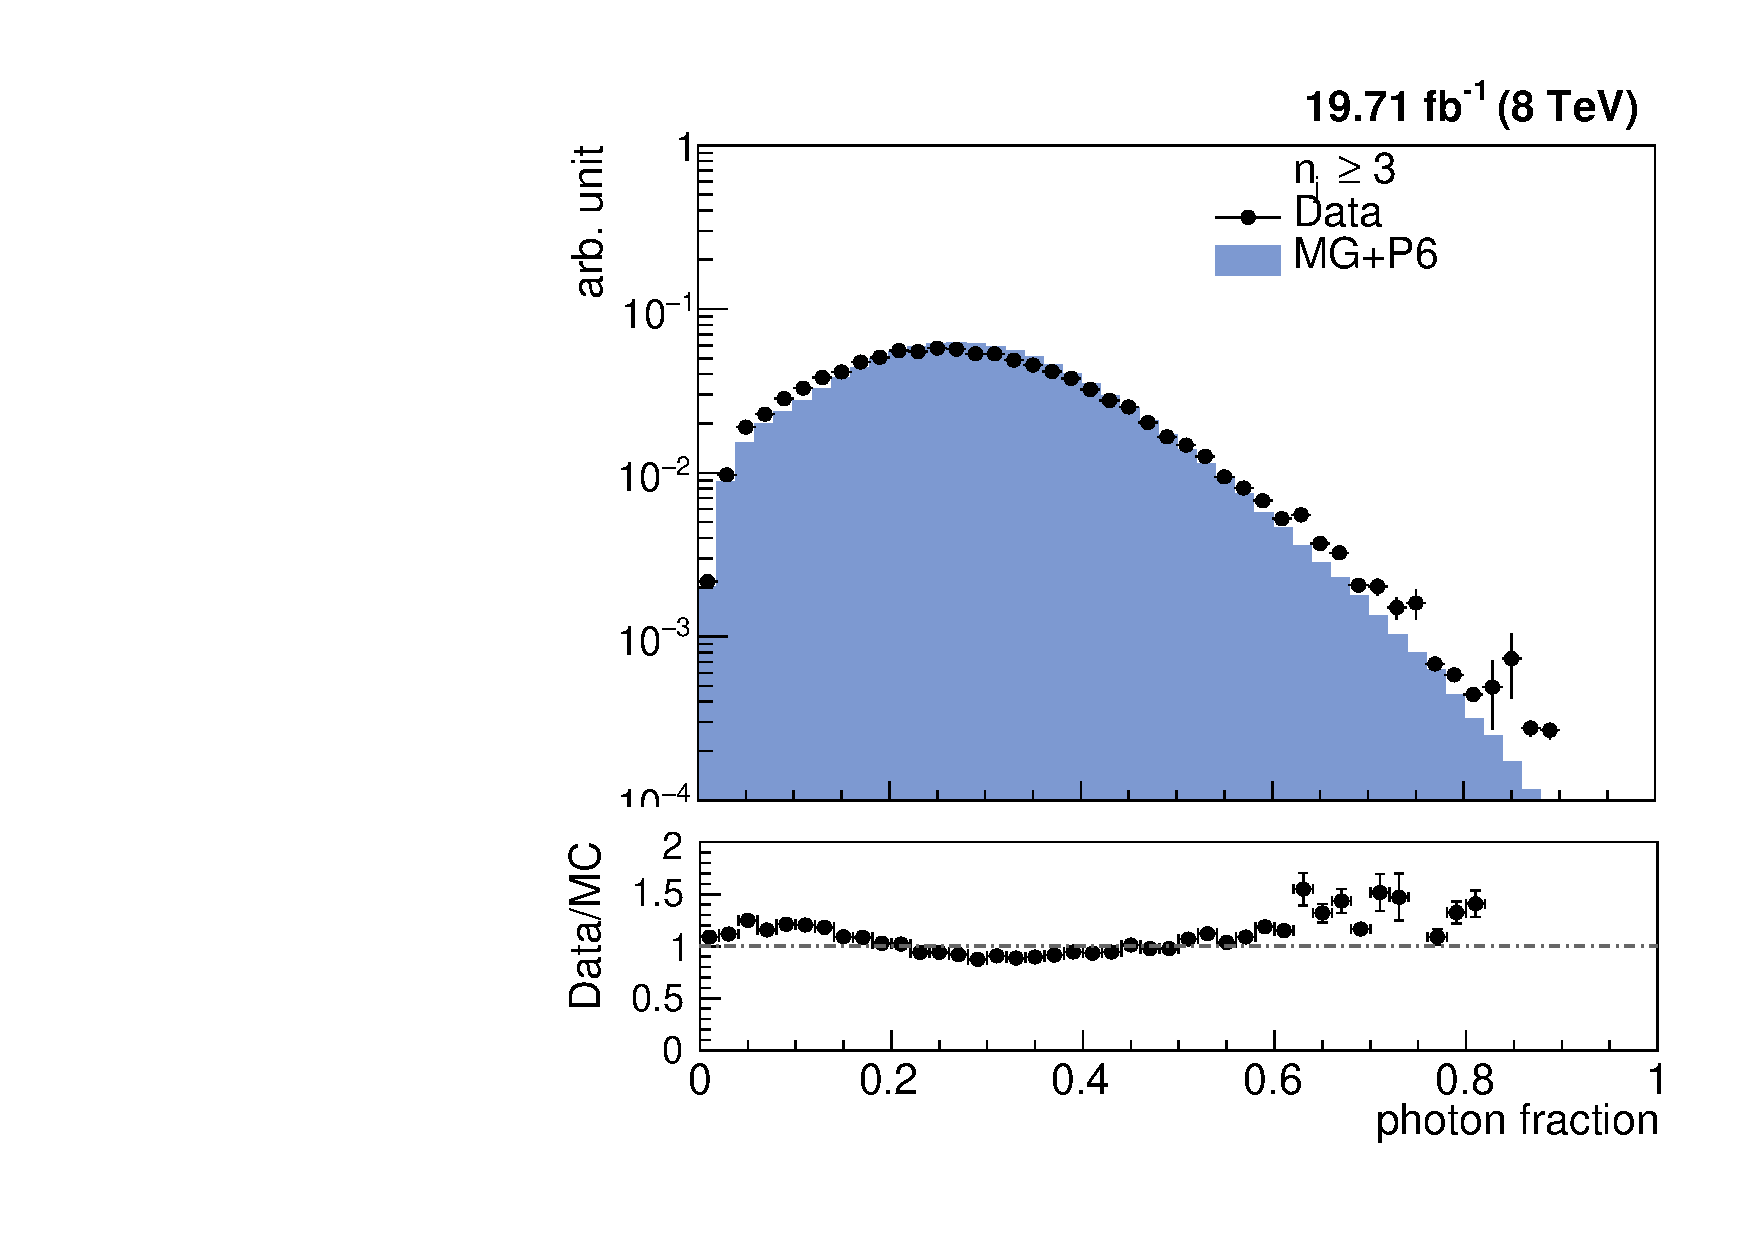
\includegraphics[width=0.5\textwidth]{Plots_HT_2_150/Qual/Comparison_PhFrac_3_HT_2_150.pdf}\\
    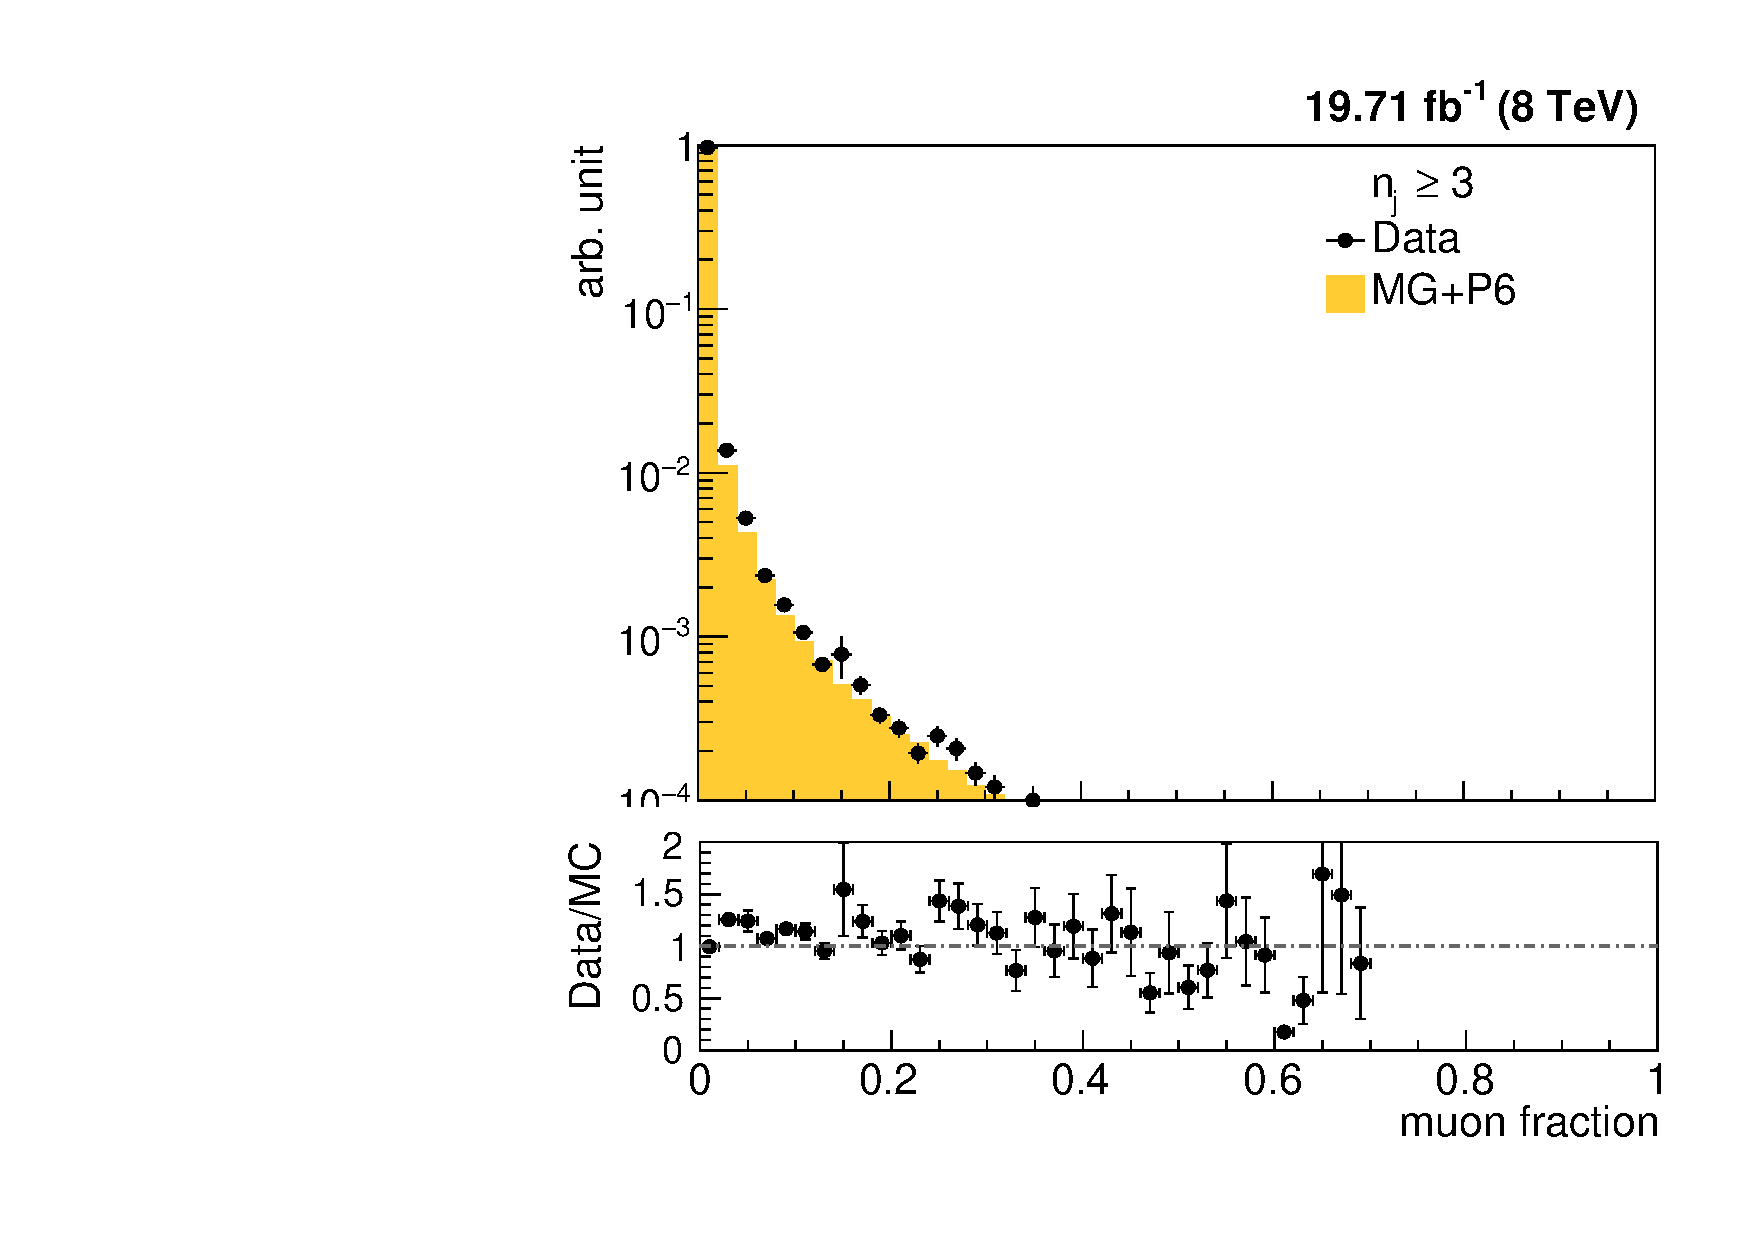
\includegraphics[width=0.5\textwidth]{Plots_HT_2_150/Qual/Comparison_MuFrac_3_HT_2_150.pdf}%
    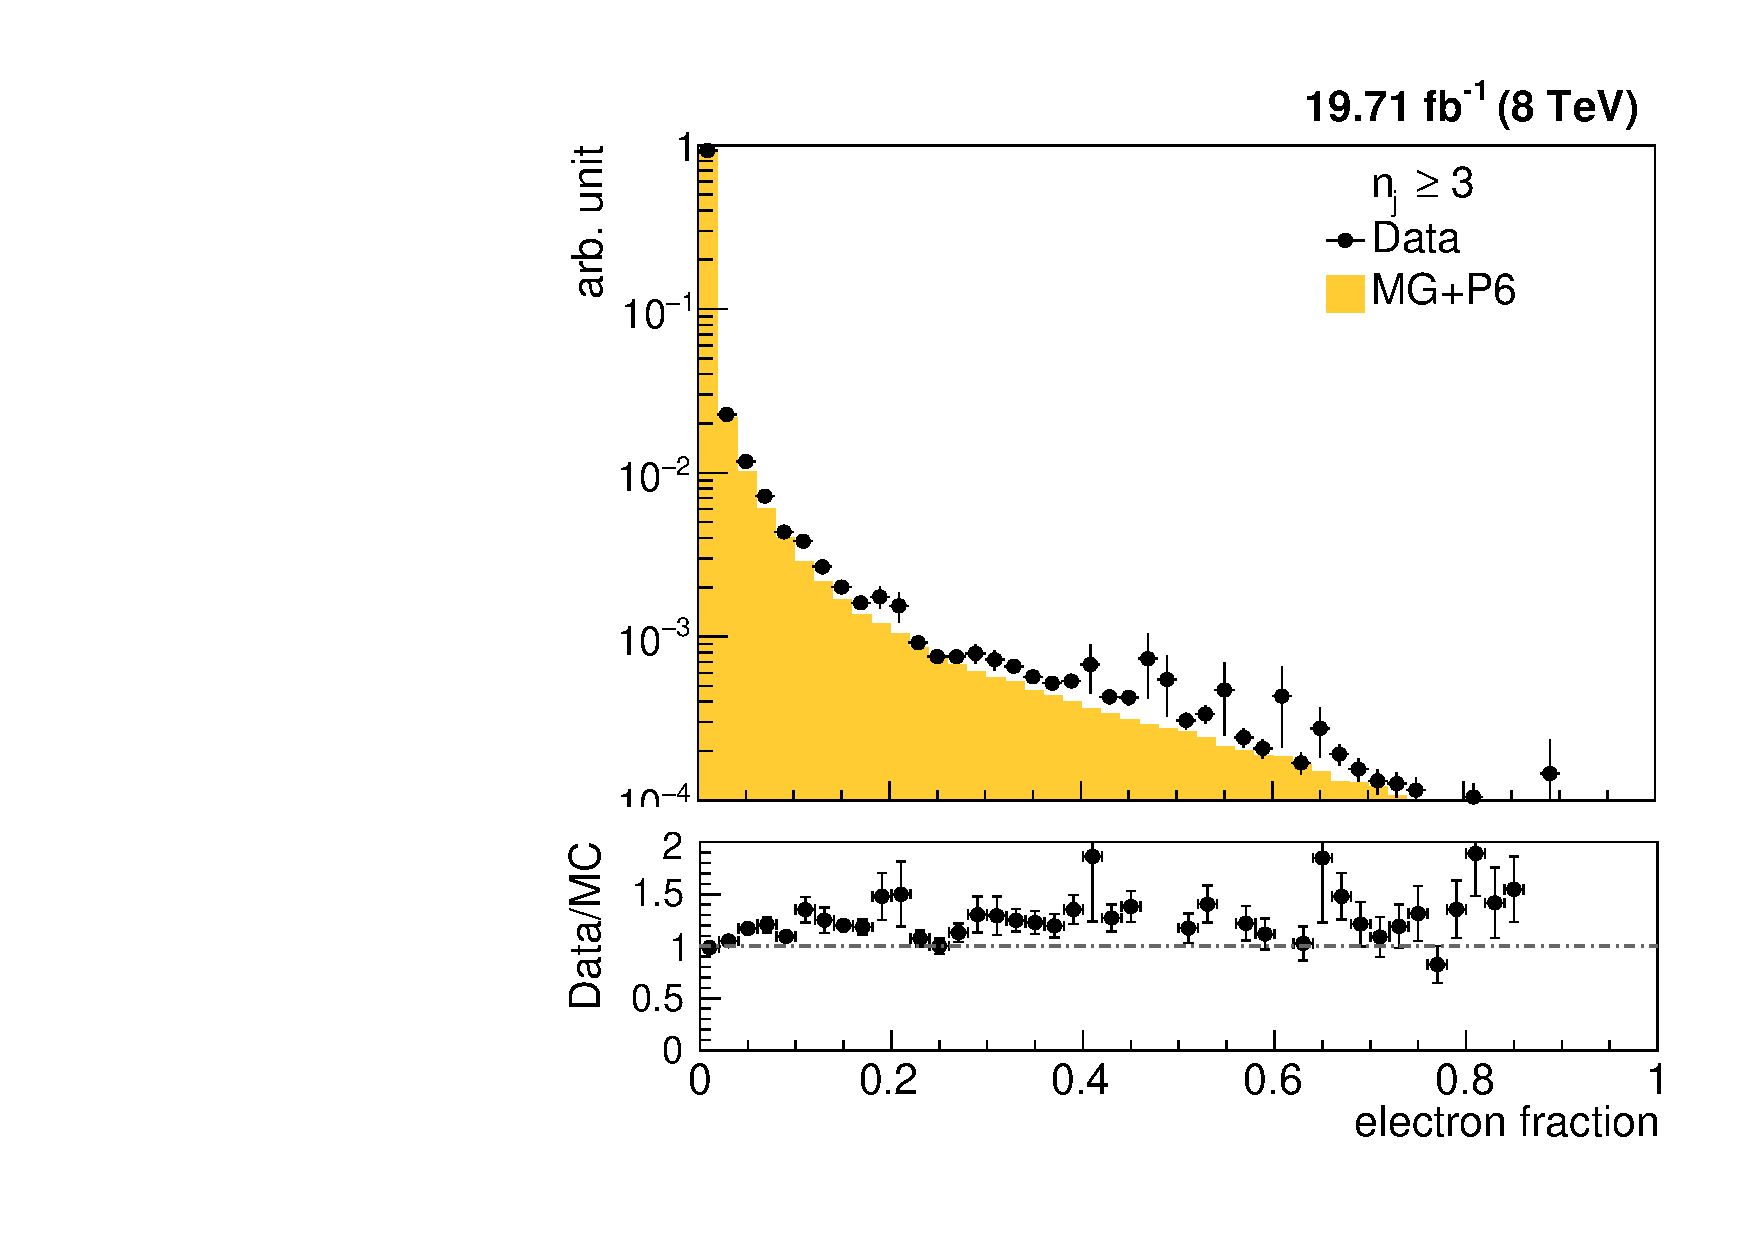
\includegraphics[width=0.5\textwidth]{Plots_HT_2_150/Qual/Comparison_ElFrac_3_HT_2_150.pdf}\\
    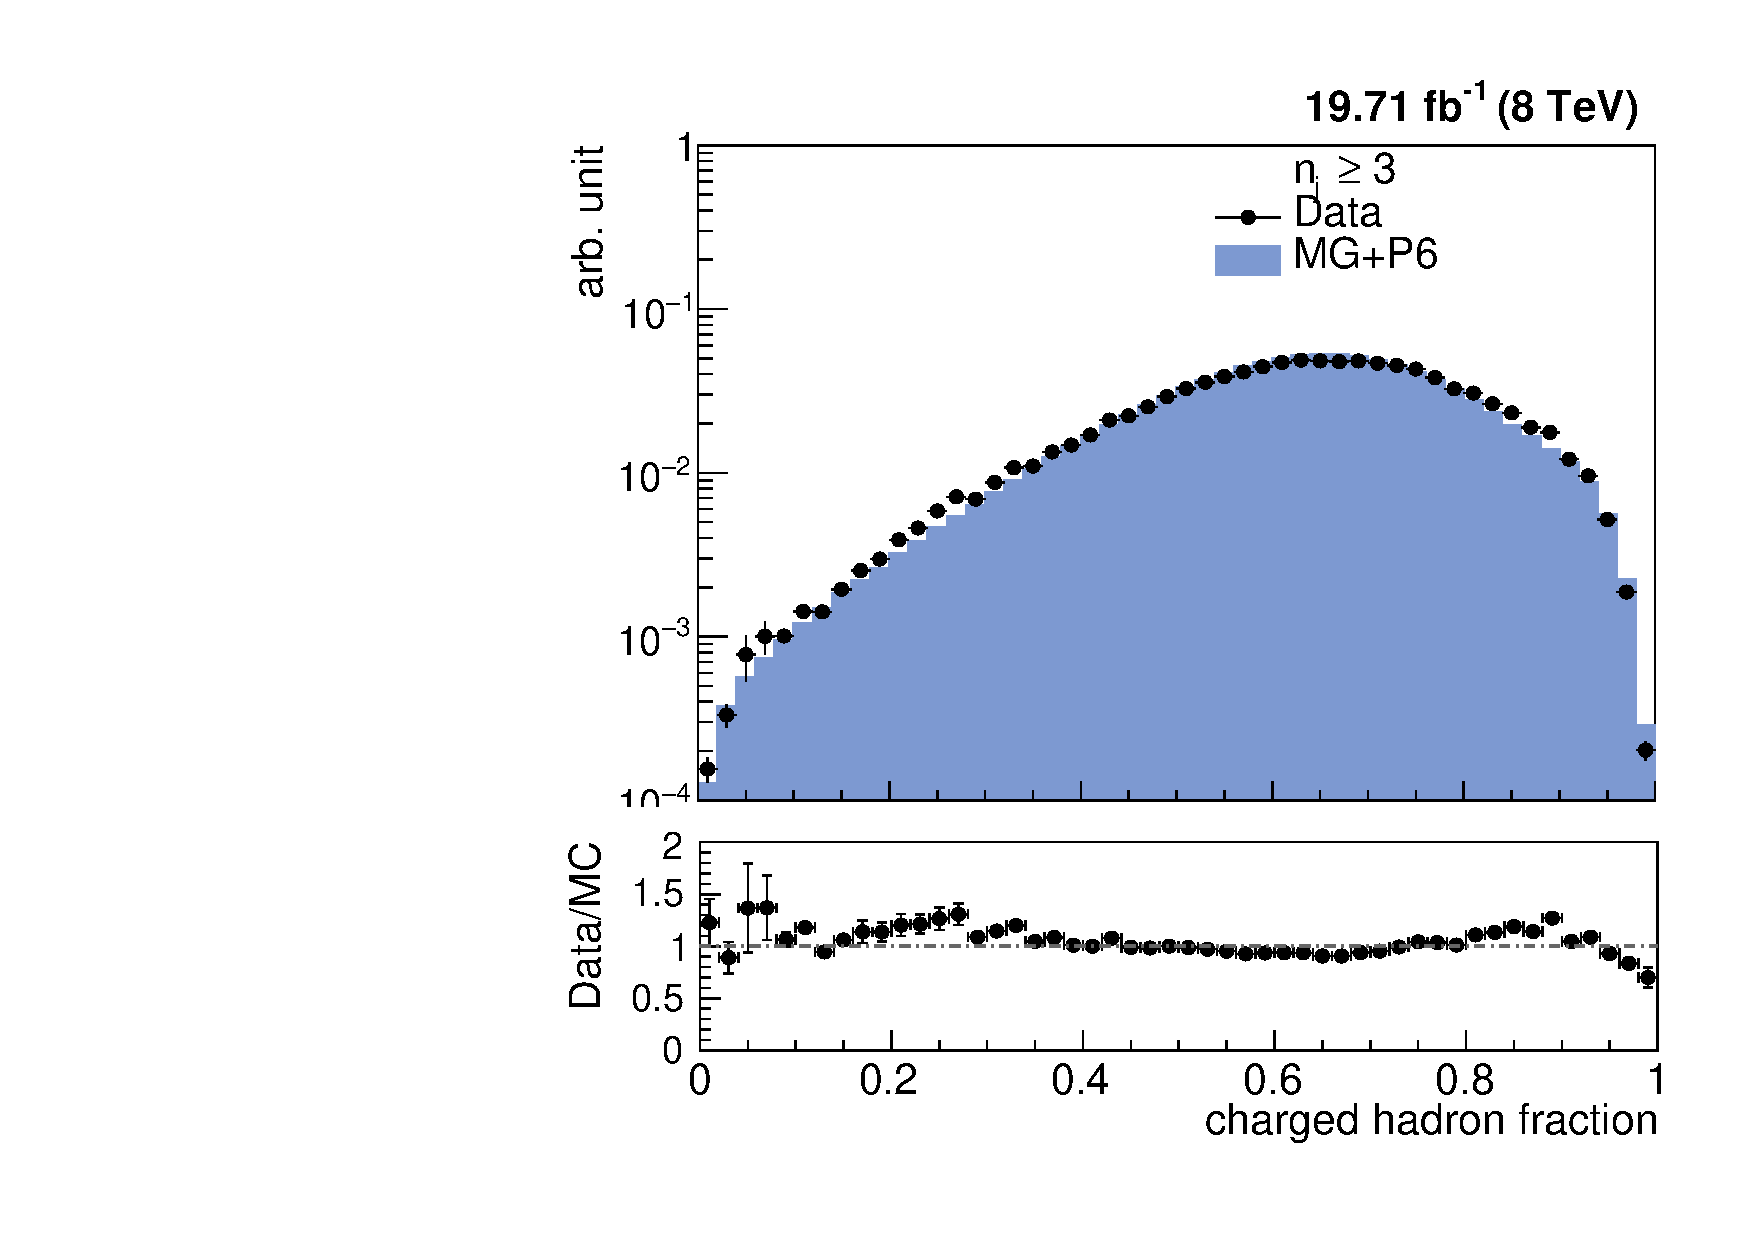
\includegraphics[width=0.5\textwidth]{Plots_HT_2_150/Qual/Comparison_ChHadFrac_3_HT_2_150.pdf}%
    \caption{The fractions of jet constituents as observed in data and simulated events for different types of PF candidates for inclusive 3-jet events. Data and simulation are normalized to the same number of events. The distributions are shown after the application of the jet ID.}
    \label{fig:qual3}
  \end{center}
\end{figure} 

\subsection{Pile-up reweighting}
The official Monte-Carlo samples are generated with distributions for the number of pileup interactions which is meant to roughly cover, 
though not exactly match the conditions expected for each data-taking period. To still get comparable pile-up distributions in data and 
simulated events, the simulated events are reweighted with a weight $\rm{ w_{PU}}$ to match the distribution in data :

\begin{equation}
  \rm{w_{PU} = \frac {N_{data} (N_{PU},est.)/\sum N_{data}} {N_{MC} (N_{PU},truth)/\sum N_{MC}}}
\end{equation}

Figure~\ref{fig:pileup} shows the number of reconstructed vertices before and after reweighting. The significant mismatch of the pile-up 
distributions in data and simulated events, which is present before the reweighting, completely vanishes.

\begin{figure}[!htbp]
  \begin{center}
    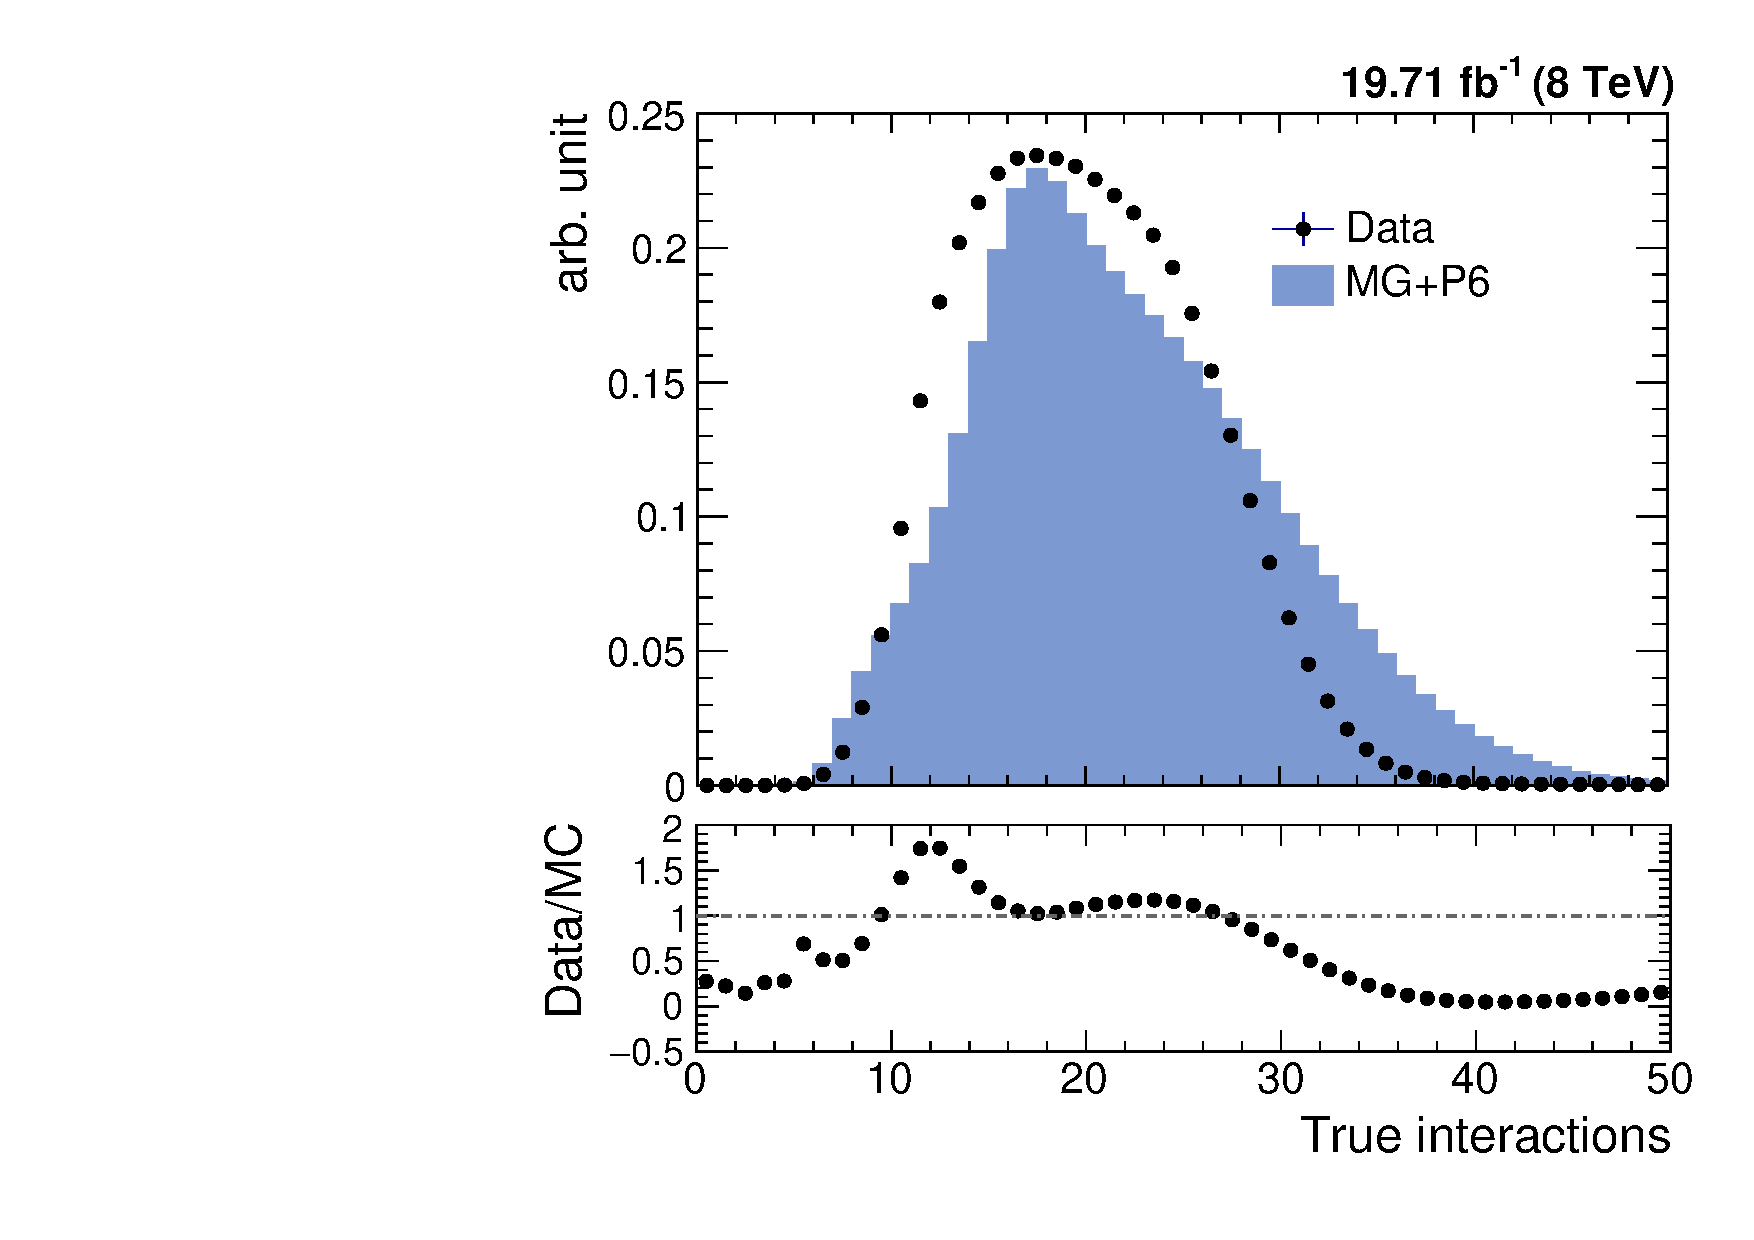
\includegraphics[scale = 0.4]{Plots_HT_2_150/Nvertices.pdf}%
    %\hspace{5mm}
    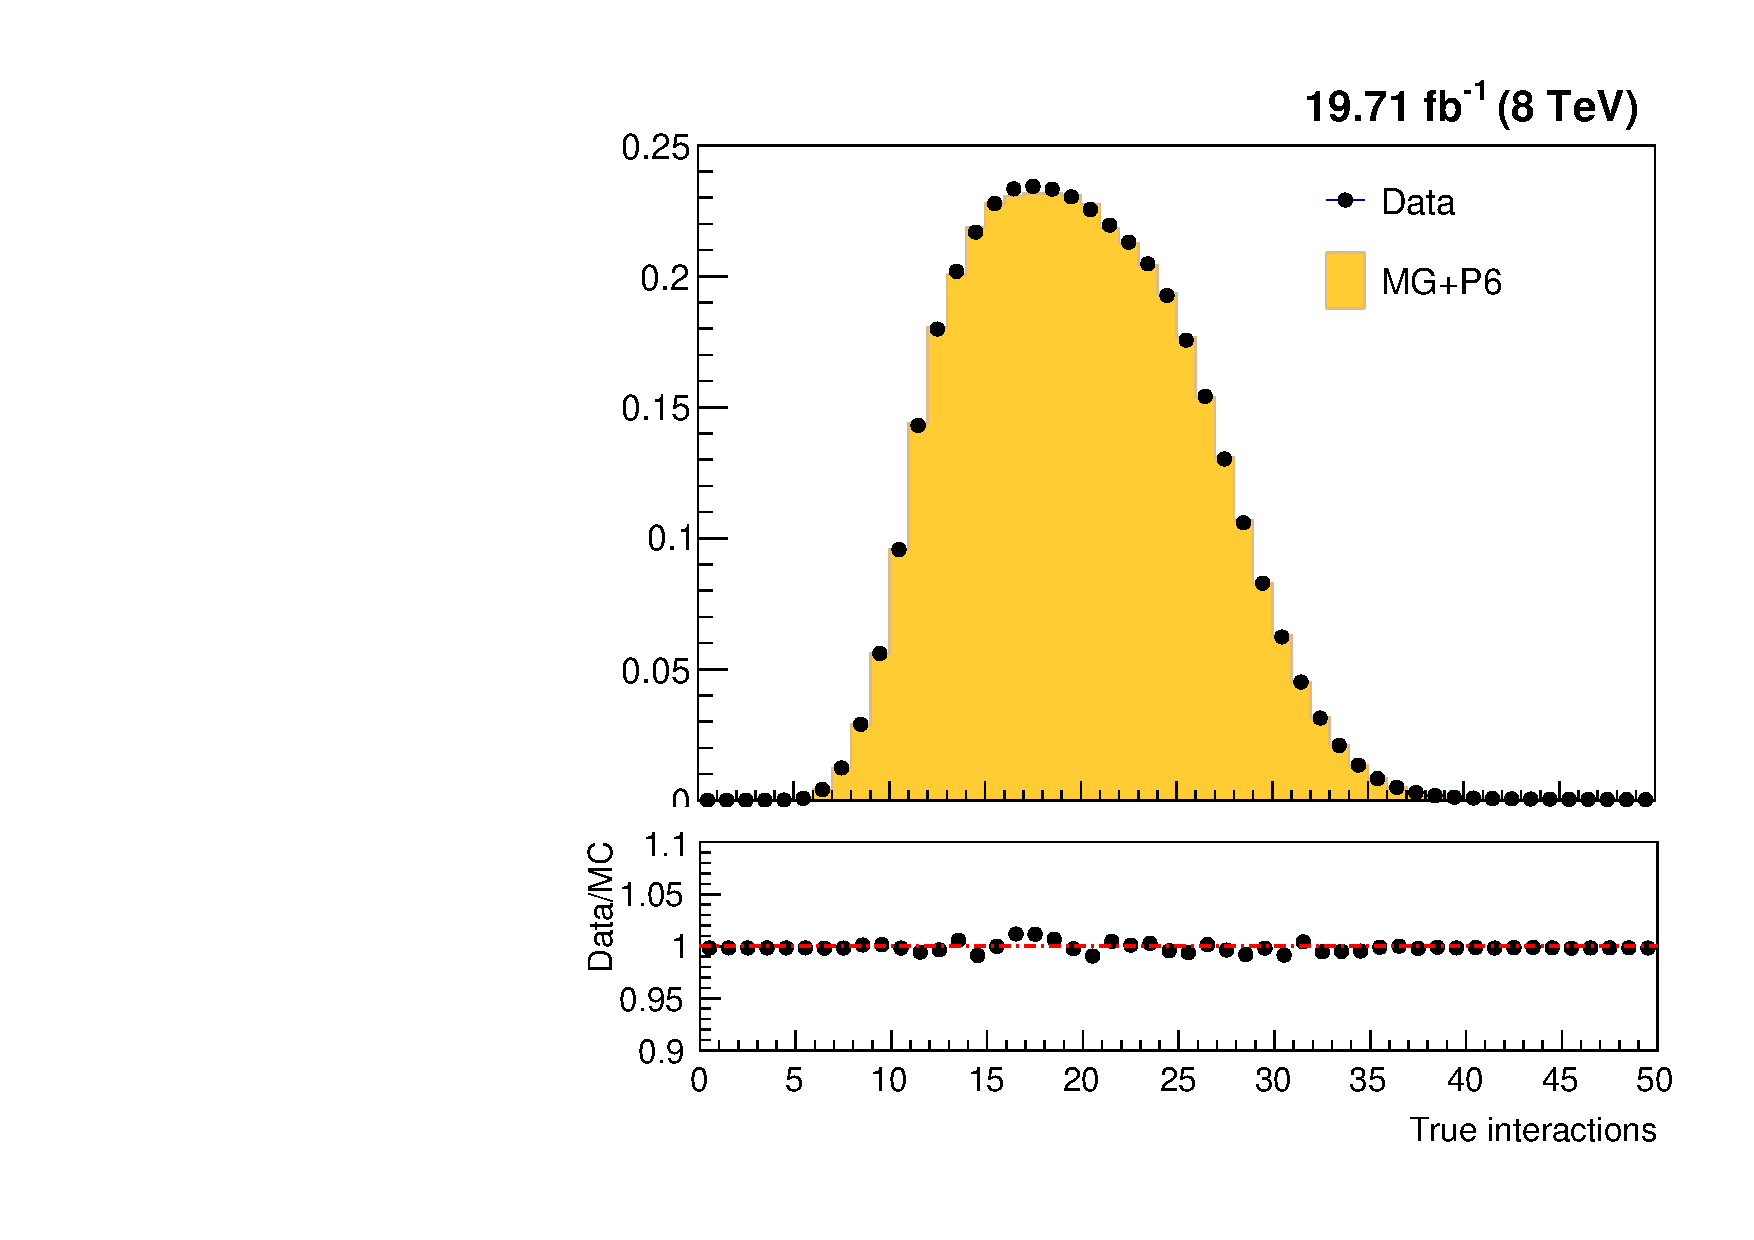
\includegraphics[scale = 0.4]{Plots_HT_2_150/Nvertices_weight.pdf}
    \caption{Number of reconstructed vertices in data and simulated events before (left) and after (right) the pile-up reweighting.}
    \label{fig:pileup}
  \end{center}
\end{figure}

\section{Kinematic Distributions}

\subsection{Differential cross section and ratios}
The inclusive differential multijet cross sections are measured as a
function of the average transverse momentum, \httwo =
$\frac{1}{2}(p_{T,1} + p_{T,2})$ where $p_{T,1}$ and $p_{T,2}$ denote
the transverse momenta of the two leading jets, and is defined 
by the basic formula : 

\begin{equation}
  \label{inclusive_formula}
        {\dd{\sigma}{\big(\httwo\big)}} = \frac{1}{\epsilon\lumi_{\mathrm{int,eff}}}\frac{N}{\Delta\big(\httwo\big)}
\end{equation}
where

\begin{itemize}
\item \textit{N} is the number of jets counted in a bin,
\item \lumins$_{\mathrm{int,eff}}$ is the effective integrated luminosity,
\item $\epsilon$ is the product of the trigger and jet selection efficiencies (greater than 99$\%$),
\item $\Delta\big(\httwo\big)$ are the bin widths in \httwo.
\end{itemize}

The measurements are reported in units of (pb/\GeVns). The inclusive 2-jet
events results are represented by n$_{j} \geq $2, inclusive 3-jet
events results by n$_{j} \geq $3 and inclusive 4-jet
events results by n$_{j} \geq $4 in the figures.
The differential cross section is studied for inclusive 2-jet, inclusive 3-jet and inclusive 4-jet events. Then ratio $R_{mn}$ 
as a function of $\httwo$ is studied which is the ratio of the differential cross section of selected inclusive m-jet events 
to that of inclusive n-jet events in each \httwo bin (m $>$ n and m $\neq$ n), 

\begin{equation}
  \label{eqn:ratio}
  R_{mn} = \frac{\Big[{\dd{\sigma}{\big(\httwo\big)}}\Big]_{(m\textit{-}jet)}}{\Big[{\dd{\sigma}{\big(\httwo\big)}}\Big]_
    {(n\textit{-}jet)}}
\end{equation}

In this section we have detector level comparison of differential cross section of 2012 full data with NLO predictions as well as
\MadGraphF + \PYTHIAS MC simulations. Figure~\ref{fig:comp_all} shows the comparison of differential cross section as a function of \httwo 
for inclusive 2-jet events (top left) and inclusive 3-jet events (top right), for data (black solid circles), \MadGraphF + \PYTHIAS 
MC (red solid circles) and NLO (histogram). At present, for inclusive 4-jet events (bottom), the results from data and MC are available. 
NLO predictions are yet to be done for this case. Each plot also shows the ratio between the MC predictions 
and the data as well as between the NLO predictions and the data. Di-jet production is 
known to suffer from large corrections from soft gluon radiation which requires re-summation beyond fixed order perturbation theory. 
Theoretical predictions at NLO including the parton shower (NLO+PS) allow to account for these effects and obtain a better description of 
the available data. 150-200 bins are not included to avoid the infrared sensitivity for the bins next to min. \pt cut in NLO calculations 
for inclusive 2-jet events.

\begin{figure}[!htbp]
  \begin{center}
    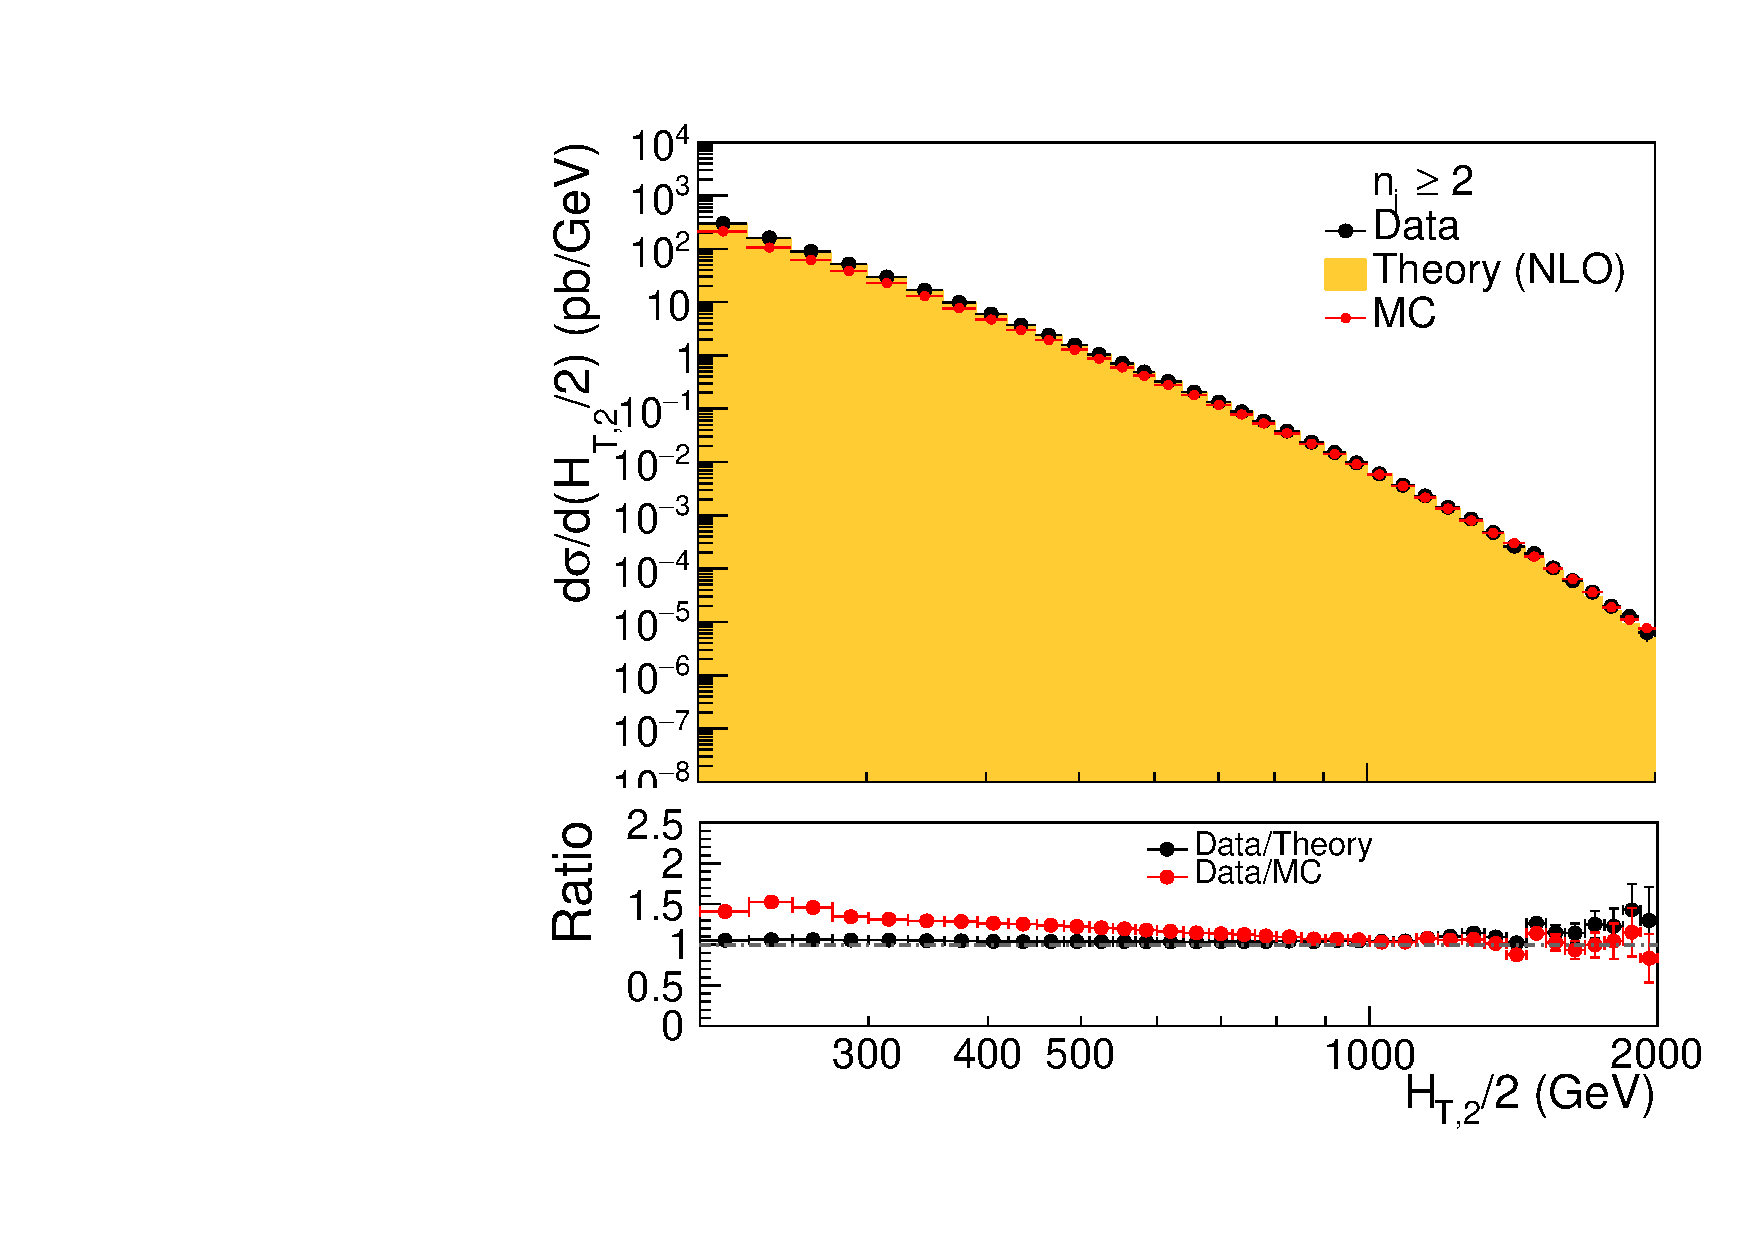
\includegraphics[scale = 0.35]{Plots_HT_2_150/Comparison_all_2_HT_2_150.pdf}%
    \hspace{4mm}
    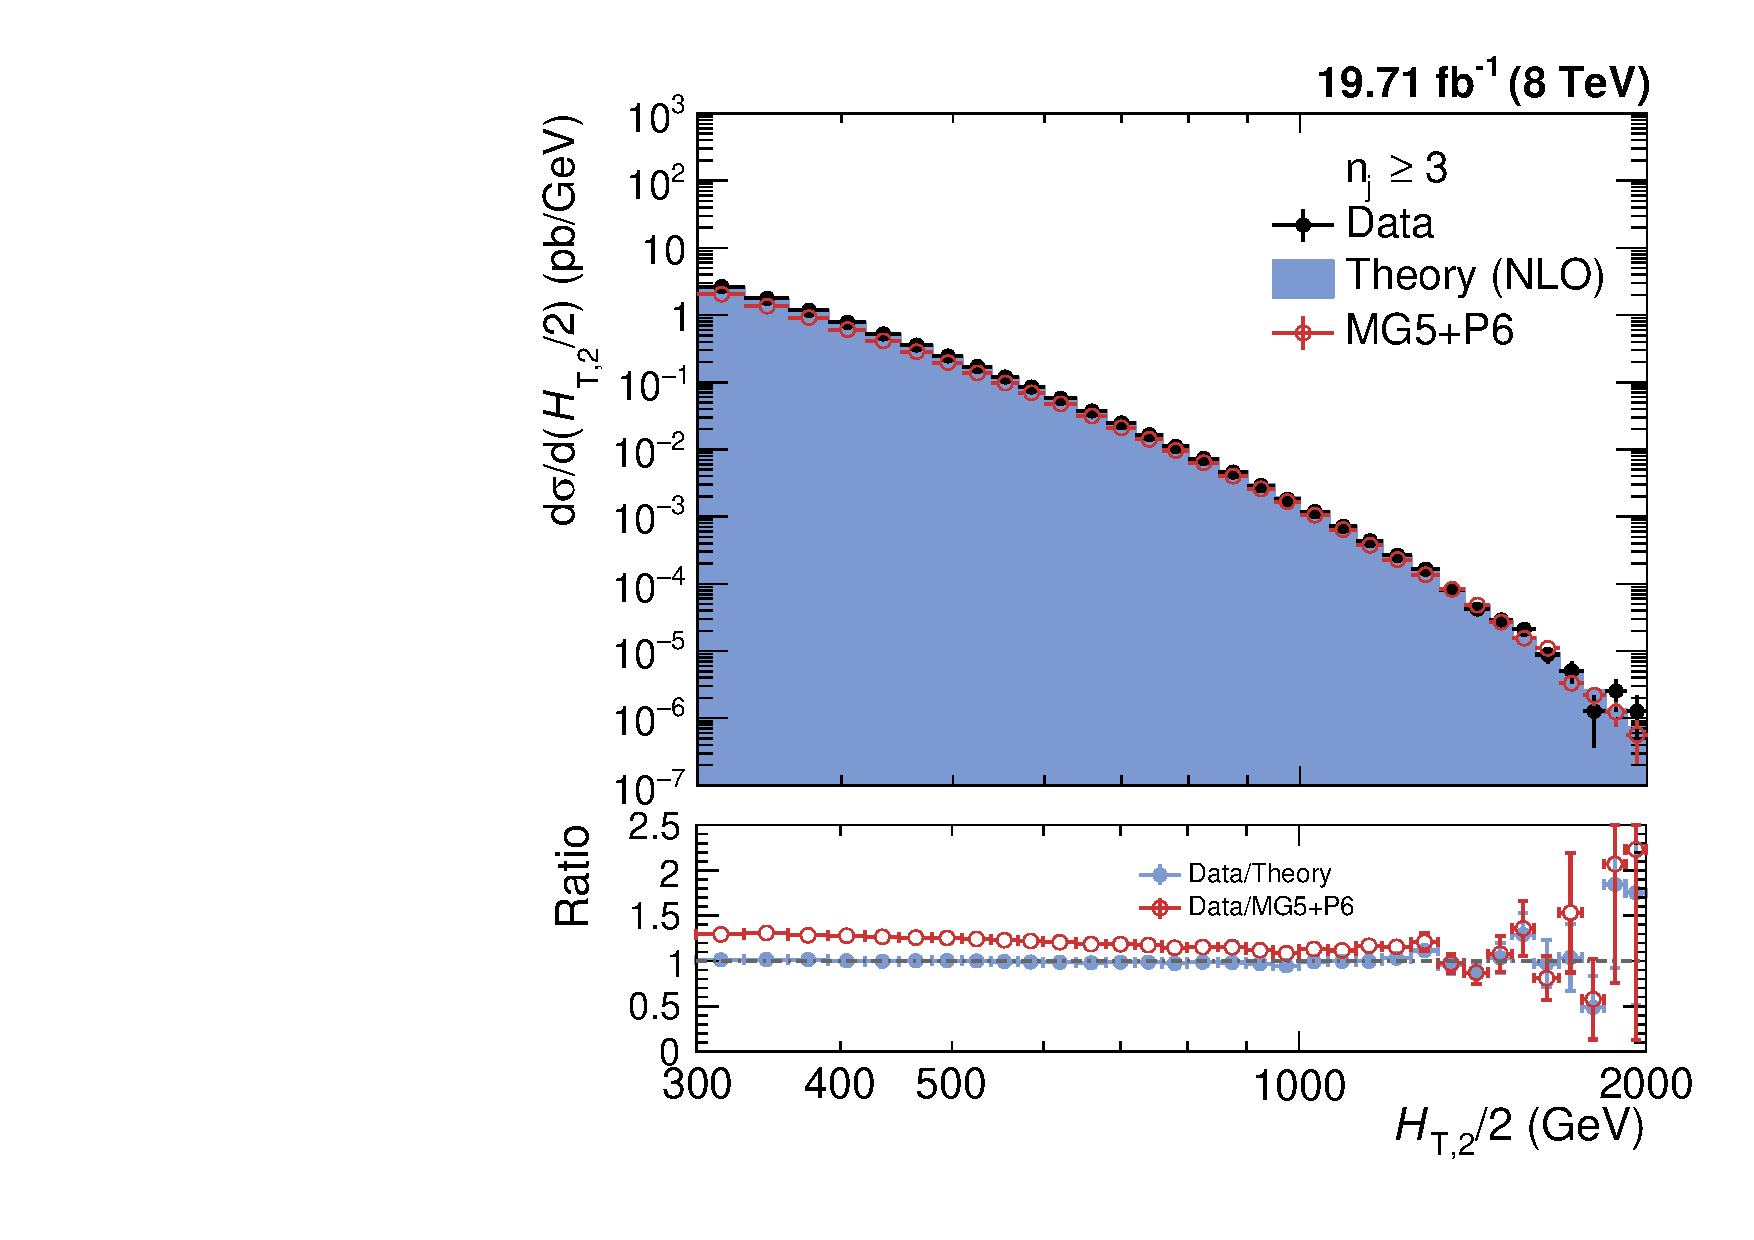
\includegraphics[scale = 0.35]{Plots_HT_2_150/Comparison_all_3_HT_2_150.pdf}\\
    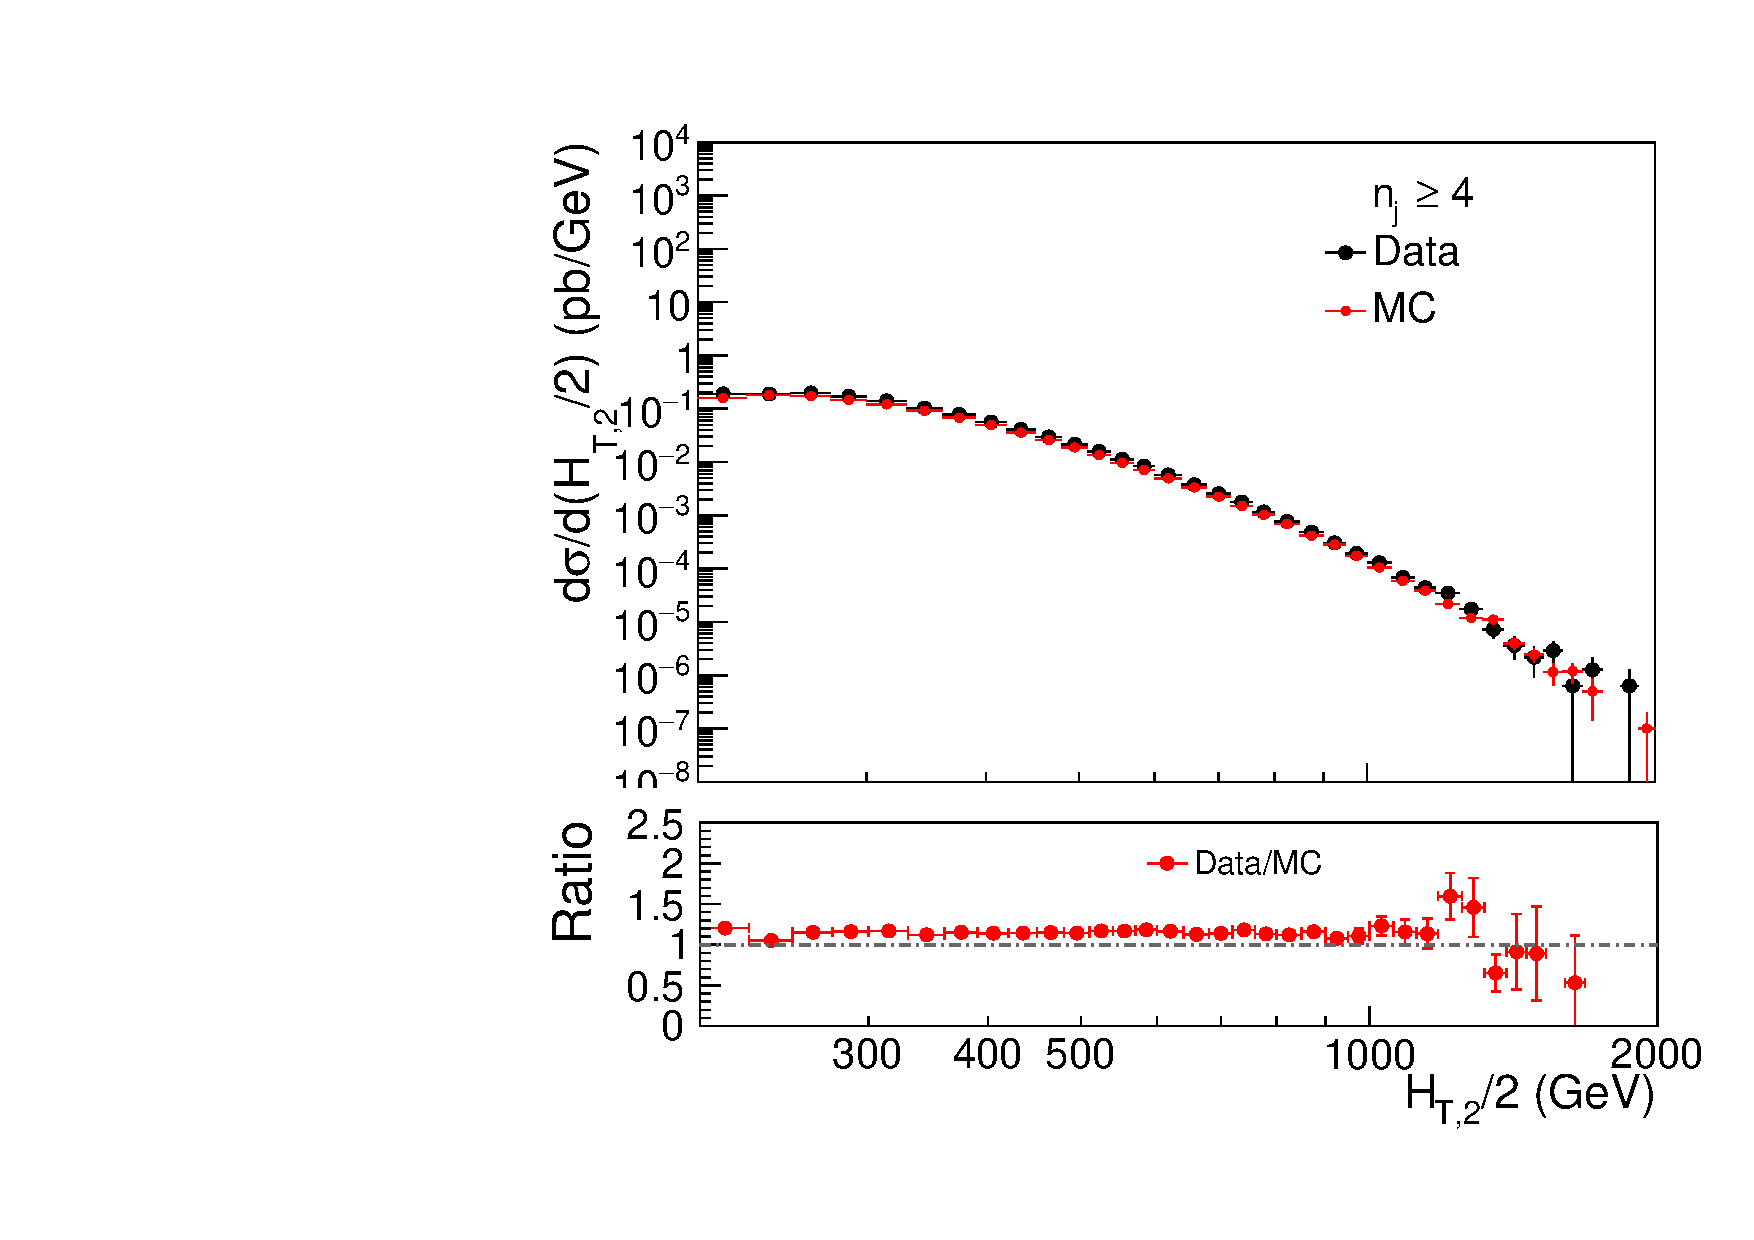
\includegraphics[scale = 0.35]{Plots_HT_2_150/Comparison_all_4_HT_2_150.pdf}
    \caption{The differential cross section as a function \httwo for inclusive 2-jet events (top left), for 
      inclusive 3-jet events (top right) and for inclusive 4-jet events (bottom), for data (black solid circles), \MadGraphF + \PYTHIAS MC 
      (red solid circles) and NLO 
      (histogram). Ratios between the MC predictions and the data as well as between the NLO predictions and the data are shown in bottom panel 
      of each plot.}
    \label{fig:comp_all}
  \end{center}
\end{figure}

\subsection{Jet Energy Resolution (JER)}
\label{subsec:Resolution}
To evaluate jet energy resolution (JER), CMS detector simulation based on 
\MadGraphF + \PYTHIAS MC event generators, is used. The jets clustered from 
stable generator particles (Gen jets) as well as from particle flow 
candidates reconstructed from the simulated detector output (Reco jets) are used. 
The studies of the JERC working group at CMS has shown that the jet energy resolution in data is actually worse than in simulation. So the 
reconstructed jet transverse momentum needs to be smeared additionally to match the resolution in data~\cite{JERC:Resolution}. Table~\ref
{resolution} shows the scaling factors (c) which need to be applied on the transverse momentum of simulated
reconstructed jets. The scaling factors depend on the absolute $\eta$ of the jet. The uncertainty on these measured scaling factors needs 
to be taken into account in a physics analysis. This is done by smearing the reconstructed jets with two additional sets of scaling factors, c$_{up}$ and c$_{down}$, that correspond to varying the factors up and down respectively, by one sigma and evaluating the impact of these new sets. 

%The Gen jets are matched to the Reco jets such that $
%\Delta$R in the $\eta$-$\phi$ plane calculated as below should be less than 0.3.

%\begin{equation}
%  \Delta R = \sqrt{\Delta \eta^2 + \Delta \phi^2}
%\end{equation}

\begin{table}[!htbp]
  \centering
  \caption{The scaling factors to be applied to the reconstructed jet transverse momentum in simulated events to match the resolution in 
    data.}
  \label{resolution}
  \vspace{2mm}
  \begin{tabular}{cccccc}
    \hline\hline
    $\eta$            & $0.0$ -- $0.5$ & $0.5$ -- $1.1$ & $1.1$ -- $1.7$ & $1.7$ --
    $2.3$ & $2.3$ -- $2.8$  \rbthm\\ \hline

    c$_{central}$    & 1.079   & 1.099   & 1.121    & 1.208   & 1.254    \rbtrr\\
    c$_{down}$       & 1.053   & 1.071   & 1.092    & 1.162   & 1.192    \rbtrr\\
    c$_{up}$         & 1.105   & 1.127   & 1.150    & 1.254   & 1.316    \rbtrr\\ 
    \hline\hline
  \end{tabular}
\end{table}

%The \pt of each reconstructed jet (\ptreco) which is matched to a generated jet is scaled using the formula : 
%
%\begin{equation}
%  \ptreco = \max \left( 0, \ptgen + c(\eta) \cdot (\ptreco - \ptgen) \right)
%\end{equation}

The reconstructed jet \pt (\ptreco) is smeared randomly using a gaussian width widened by the scaling factor (c) 

\begin{equation}
\pt \rightarrow Gauss(\mu = \pt, \sigma = \sqrt{c^2 - 1} \cdot JER^{MC_{\pt}})
\end{equation}

where $JER^{MC_{\pt}}$ is jet \pt absolute resolution

After smearing transverse momentum of each reco jet, \httwo is calculated from both generator particle jets and the particle flow jets. Then the resolution is calculated as : 

\begin{equation}
  R = \frac{Gen~\httwo}{Reco~\httwo} 
\end{equation}

\begin{figure}[!htbp]
  \begin{center}
    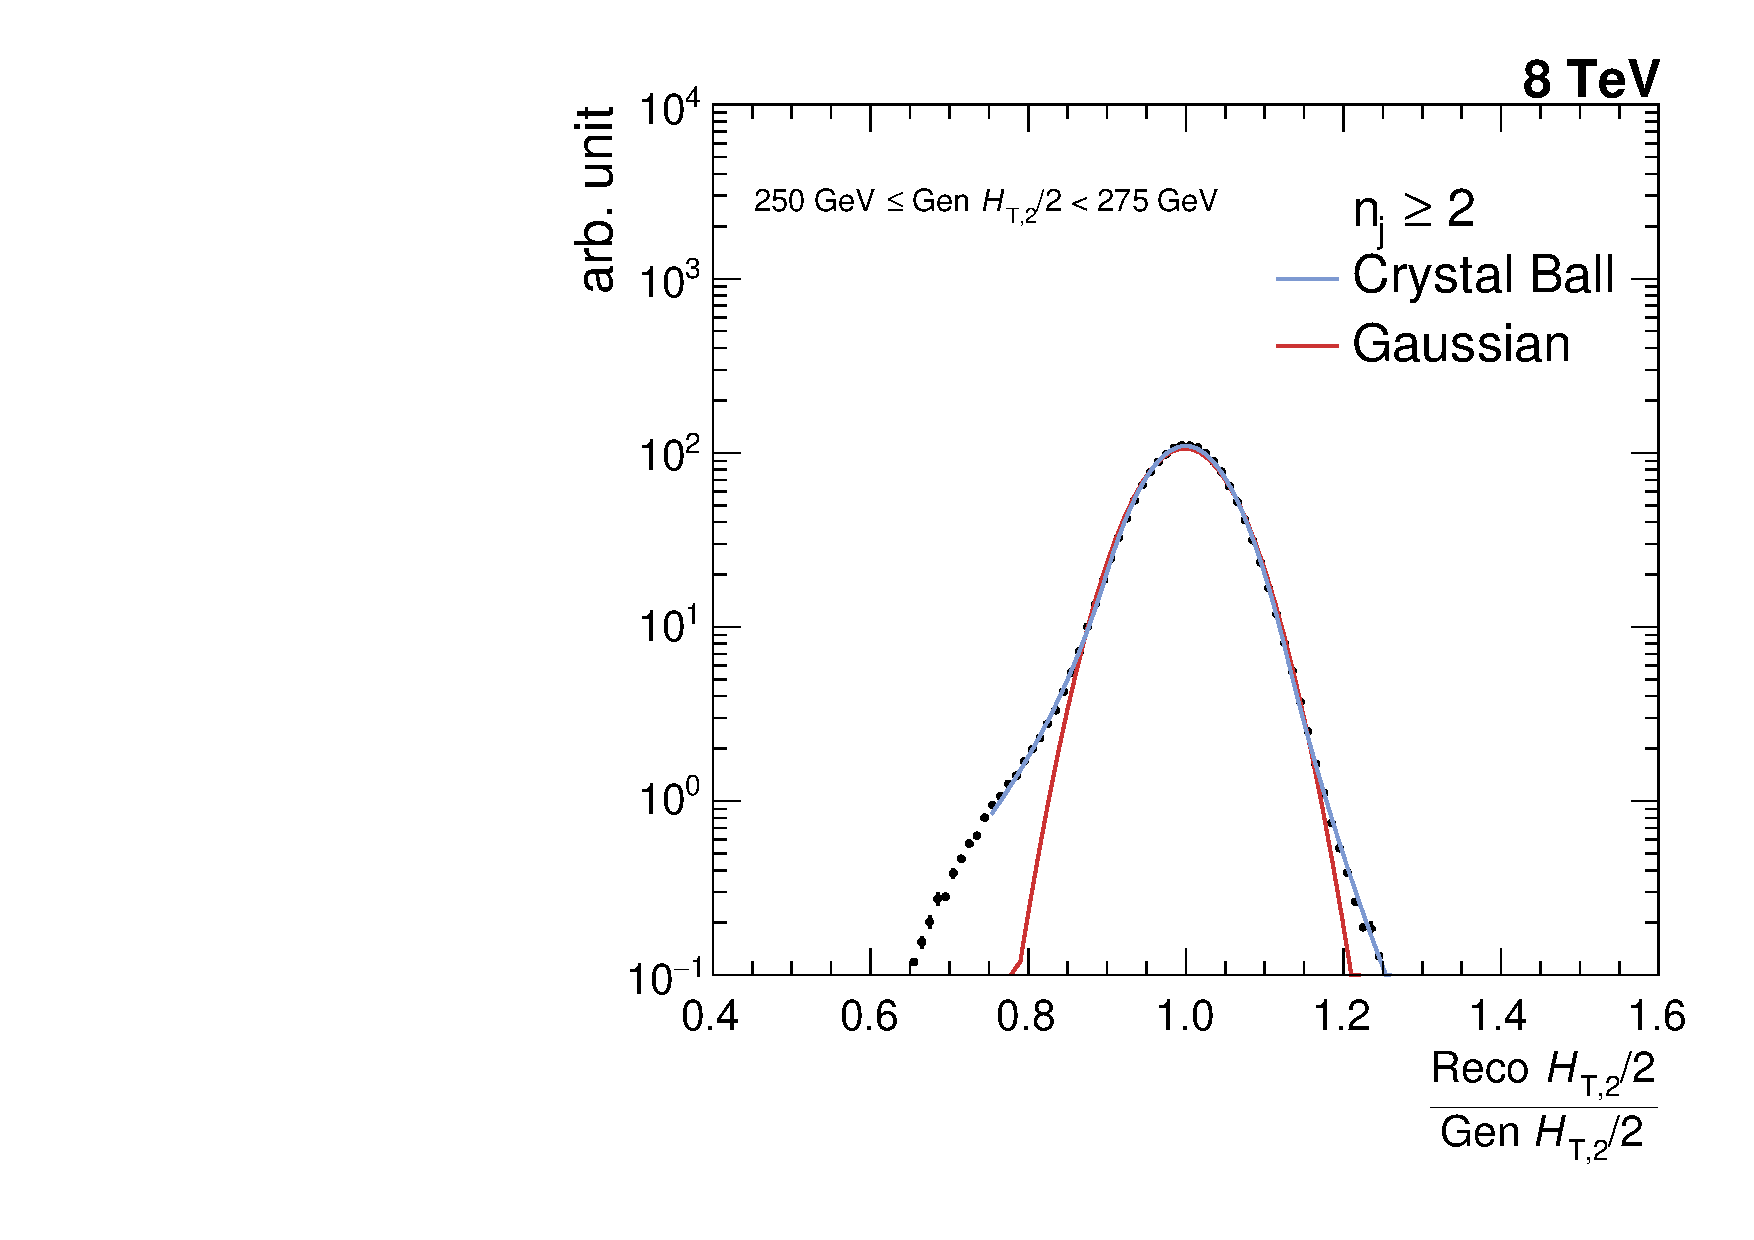
\includegraphics[scale = 0.41]{Plots_HT_2_150/Fit_Res_2_final_crystal_genbin_250-275_crystal_nomet.pdf}%
    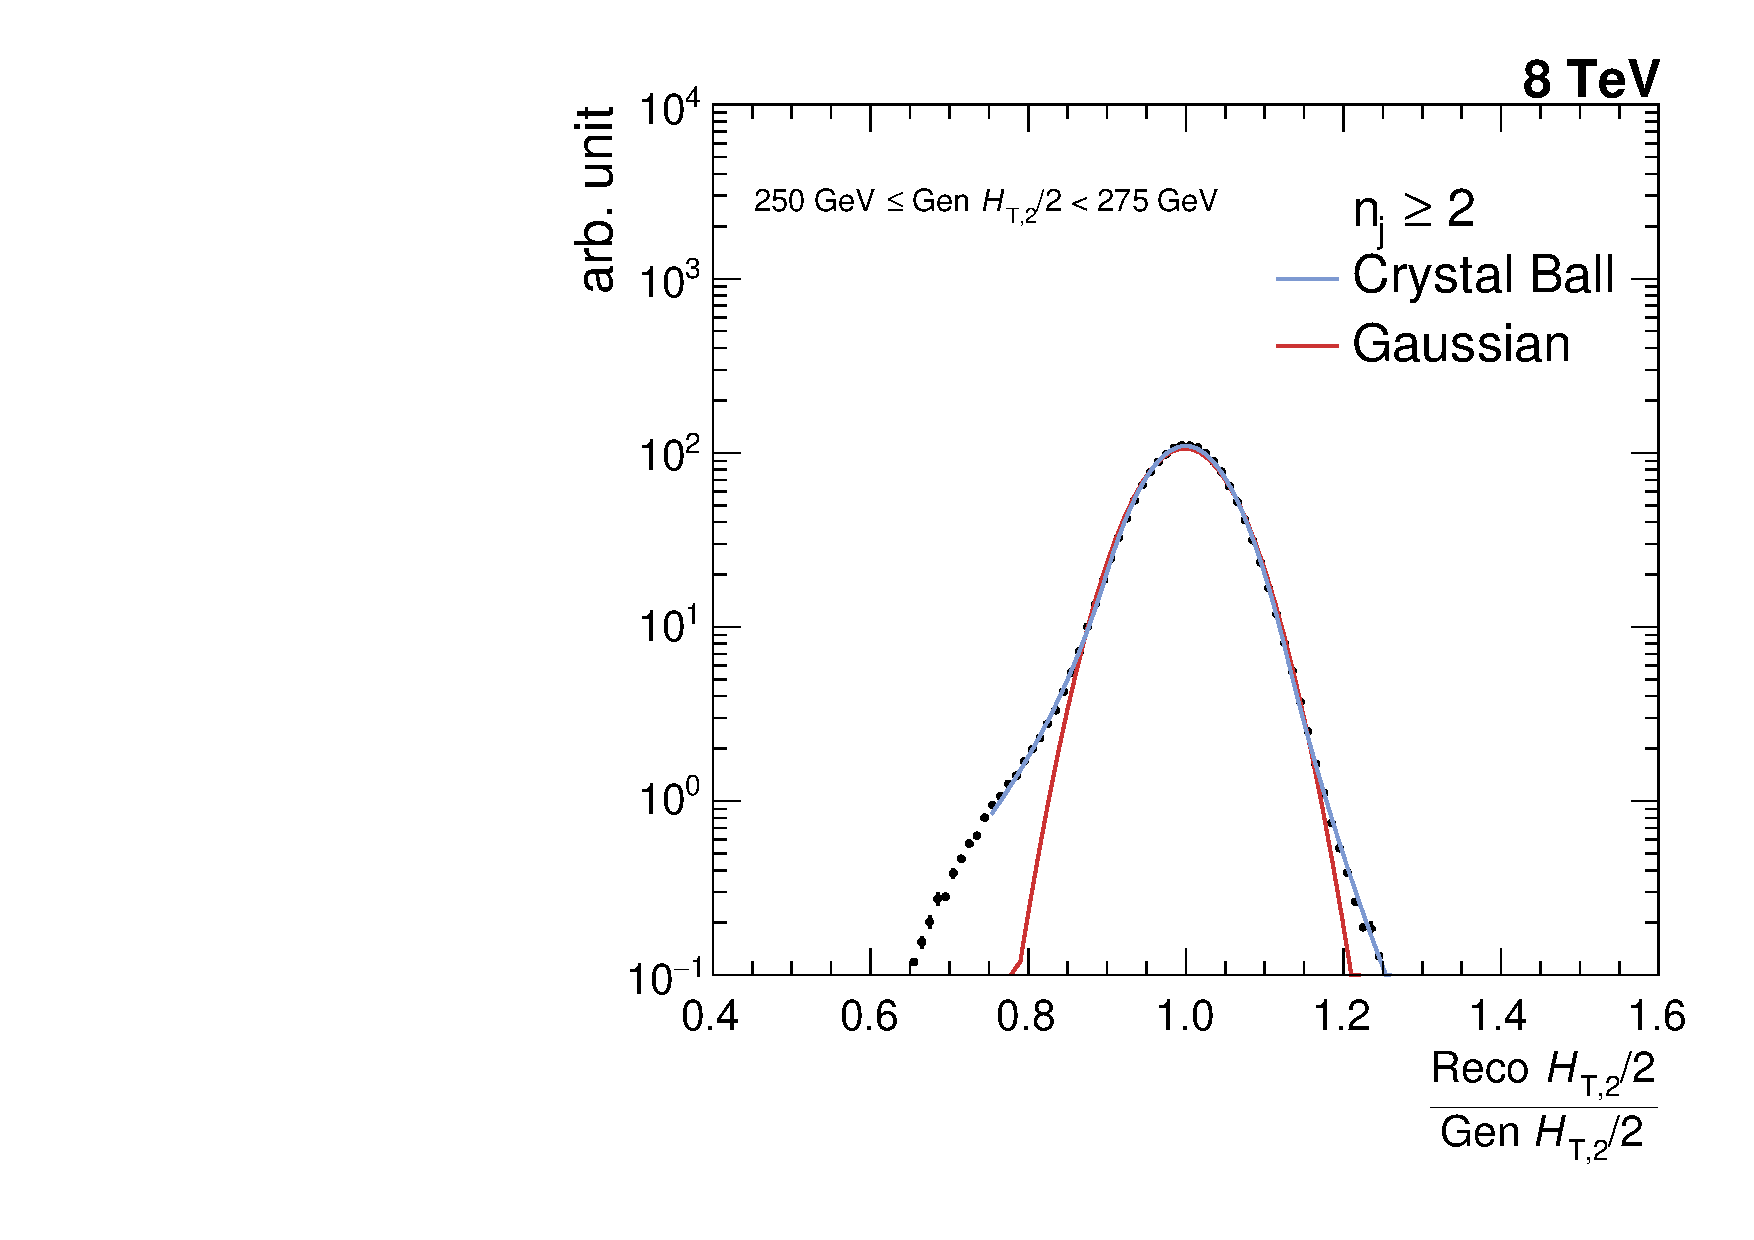
\includegraphics[scale = 0.41]{Plots_HT_2_150/Fit_Res_2_final_crystal_genbin_250-275_crystal_nomet.pdf}
    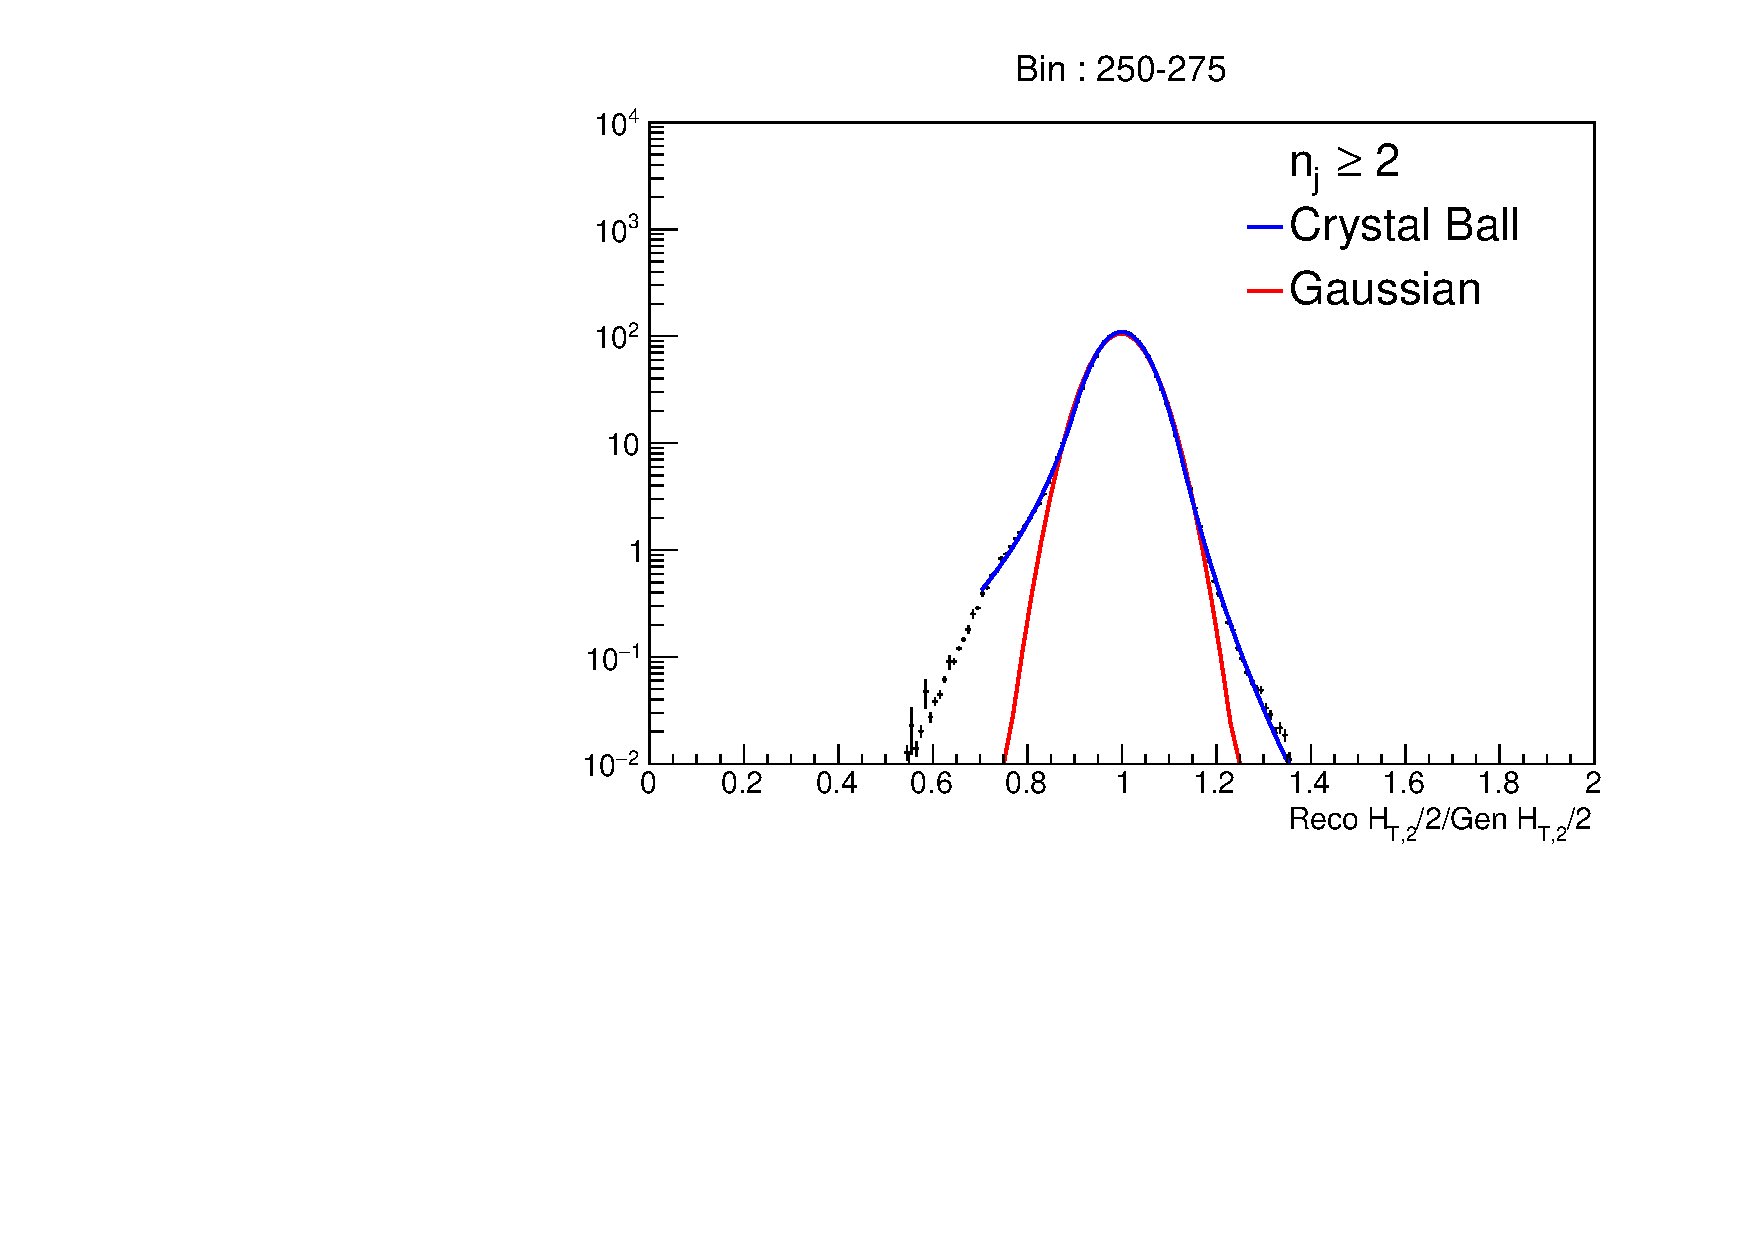
\includegraphics[scale = 0.41]{Plots_HT_2_150/Fit_Res_2_final_crystal_genbin_250-275_crystal.pdf}%
    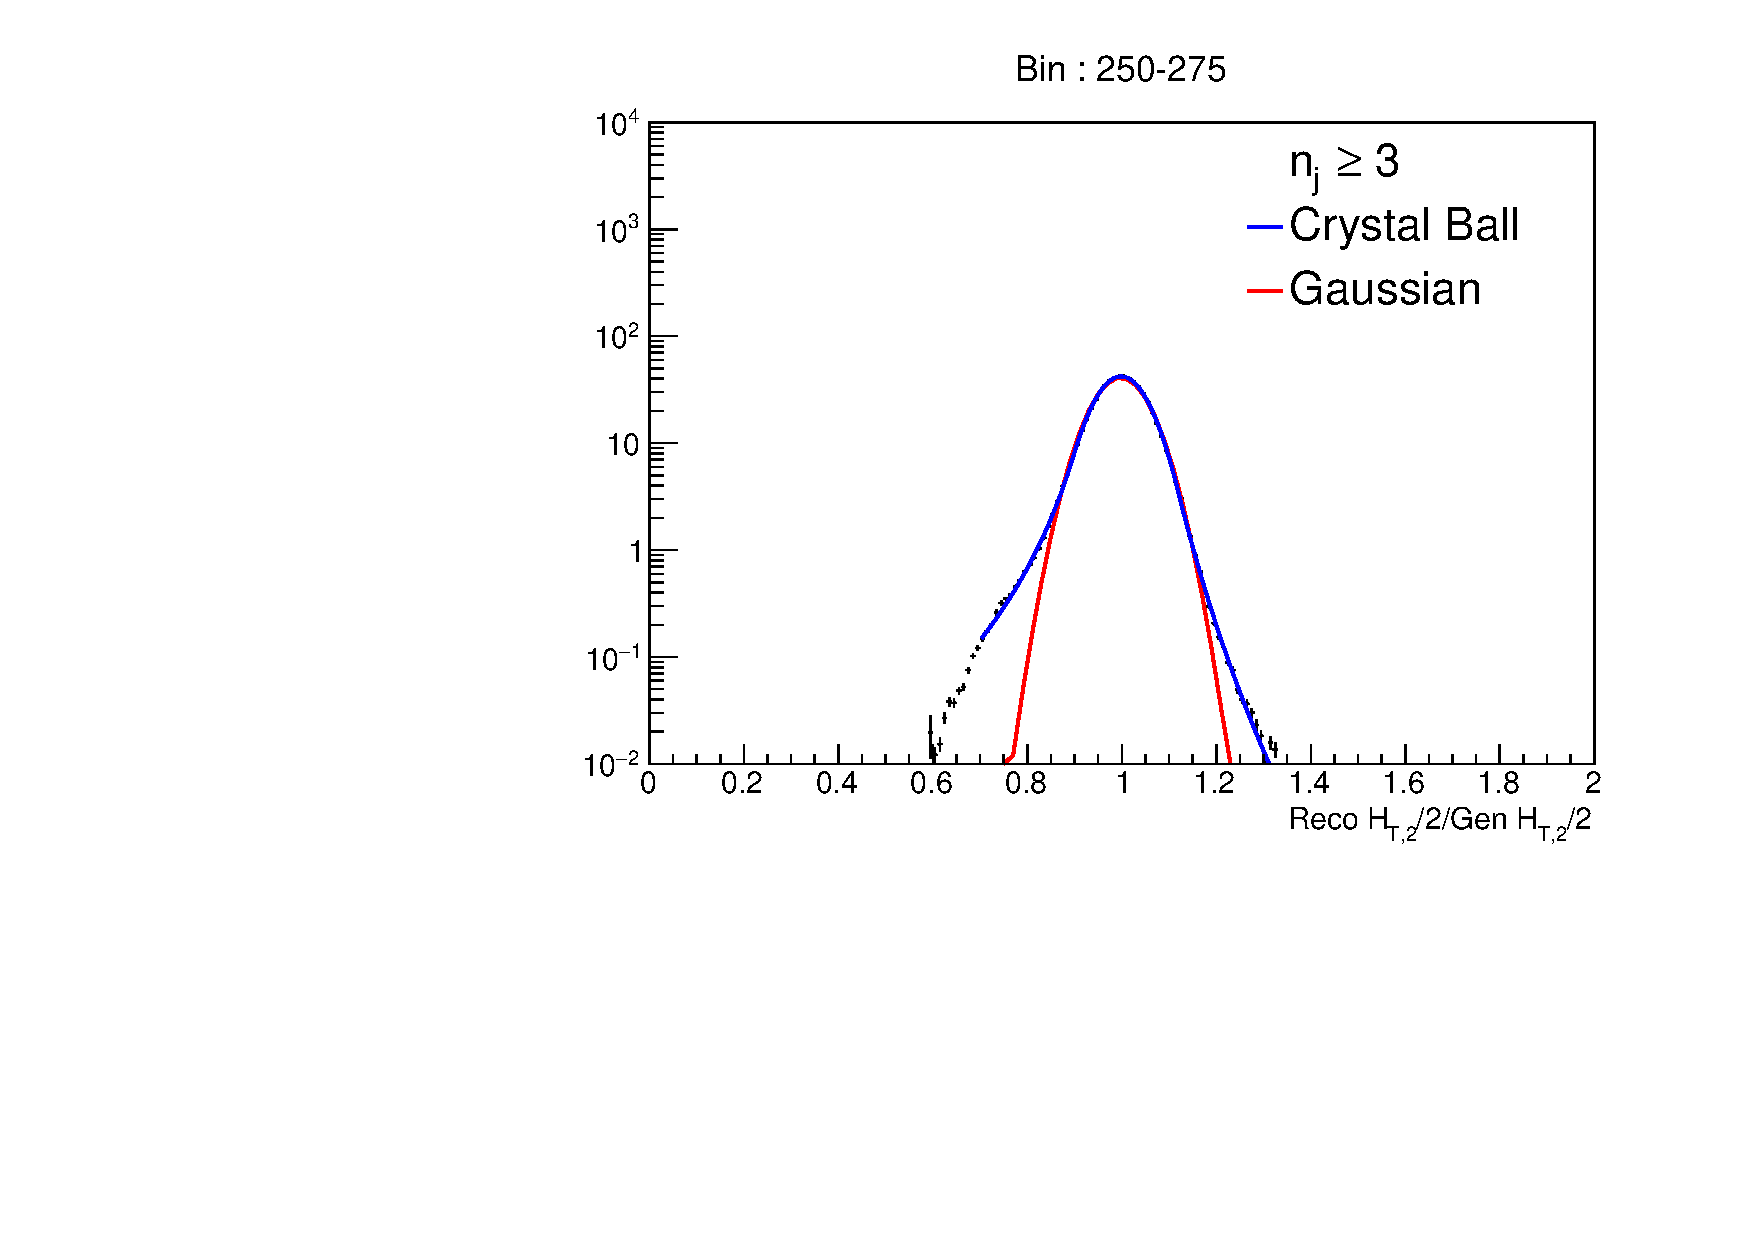
\includegraphics[scale = 0.41]{Plots_HT_2_150/Fit_Res_3_final_crystal_genbin_250-275_crystal.pdf}\\
    \caption{Fitting of the resolution distribution as a function of \httwo for inclusive 2-jet (left) and for inclusive 3-jet events 
      (right). The blue solid line shows the Crystal Ball fit of Reco \httwo/Gen \httwo in each Gen \httwo bin overlayed by Gaussian fitting the core of the resolution (red solid line). Top row shows the results without the $\frac{\ETmiss}{\sum \ET}$ cut whereas the bottom results are after applying the $\frac{\ETmiss}{\sum \ET}$ cut.}
    \label{fig:fit_gauss}
  \end{center}
\end{figure}

The width of the resolution distribution in a given Gen~\httwo bin is interpreted as the resolution. The jet resolution can in good 
approximation be described by the $\sigma$ of a Gaussian fit to the core of the jet resolution distribution. To describe the tails of the jet response distribution, a double-sided Crystal-Ball function is used.%, which is characterized by a Gaussian core with upper and lower tails each described by a power law : 

%\begin{equation}
%  f(u:N,\mu,\sigma,a_1,p_1,a_2,p_2)=\begin{cases}
%    A_1(B_1-u)^{-p_1}, & \text{if $u<-a_1$},\\
%    ~~~~~~~~~e^{-u^2/2}, & \text{if $-a_1 \leq u \leq a_2$},\\
%    A_2(B_2+u)^{-p_2}, & \text{if $u>a_2$},\\
%  \end{cases}
%\end{equation}
%where,
%\begin{equation} 
% u& \equiv \frac {x-\mu}{\sigma}, \\
% A_i&  \equiv \bigg(\frac{p_i}{|a_i|}\bigg)^{p_i} \cdot e^{-a_i^2/2}, \\
% B_i&  \equiv \bigg(\frac{p_i}{|a_i|}\bigg) - |a_i|, \\
%\end{equation} 

A fit example for one Gen~\httwo bin is shown in Figure~\ref{fig:fit_gauss} for inclusive 2-jet (left) and inclusive 3-jet events(right).  Here the black dots represent the jet resolution 
distribution, the double-sided Crystal-Ball fit (blue solid line) is overlayed by the Gaussian fit (red solid line). Top 
row shows the results without the $\frac{\ETmiss}{\sum \ET}$ cut whereas the bottom row results are after applying the $\frac{\ETmiss}{\sum 
  \ET}$ cut. It is observed that this cut is not affecting the Reco/Gen tails. %and double-sided Crystal-Ball fits are overlayed. Note that the Gaussian parameter $\mu$ and $\sigma$ are determined from the Gaussian-only fit and then fixed when determining the additional four parameters of the double-sided Crystal-ball : a$_{1}$, p$_{1}$, a$_{2}$ and p$_{2}$.

The width of the distributions in each Gen~\httwo bin is then plotted as a function of Gen~\httwo. From Figure~\ref{fig:res_comp}, it has 
been observed that the Crystal Ball function better describes the measured distributions, especially in the low-\httwo region where the non-
Gaussian tails are more pronounced. So we have switched to the Crystal Ball function to determine the resolution.

\begin{figure}[!htbp]
  \begin{center}
    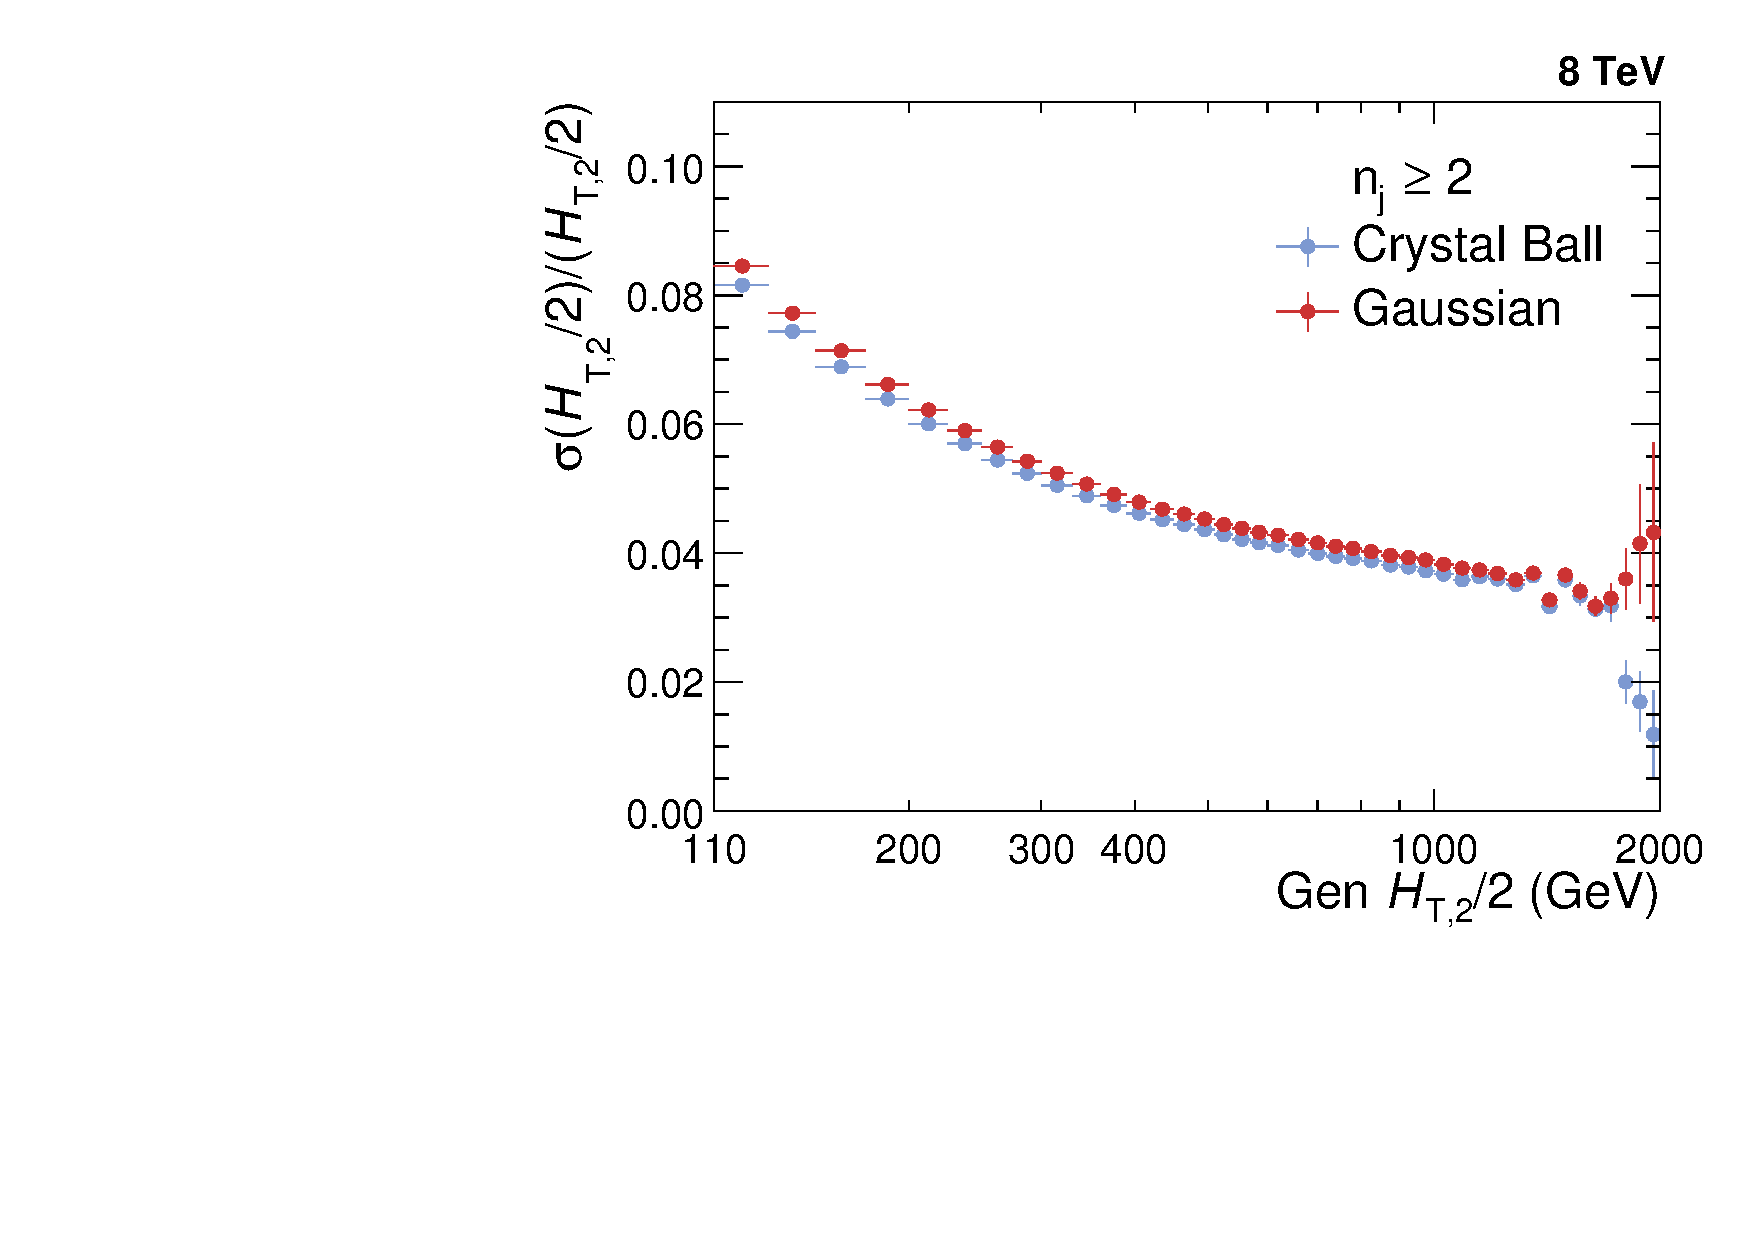
\includegraphics[width=0.5\textwidth]{Plots_HT_2_150/Comparison_Resolution_Crystal_Gauss_2.pdf}%
    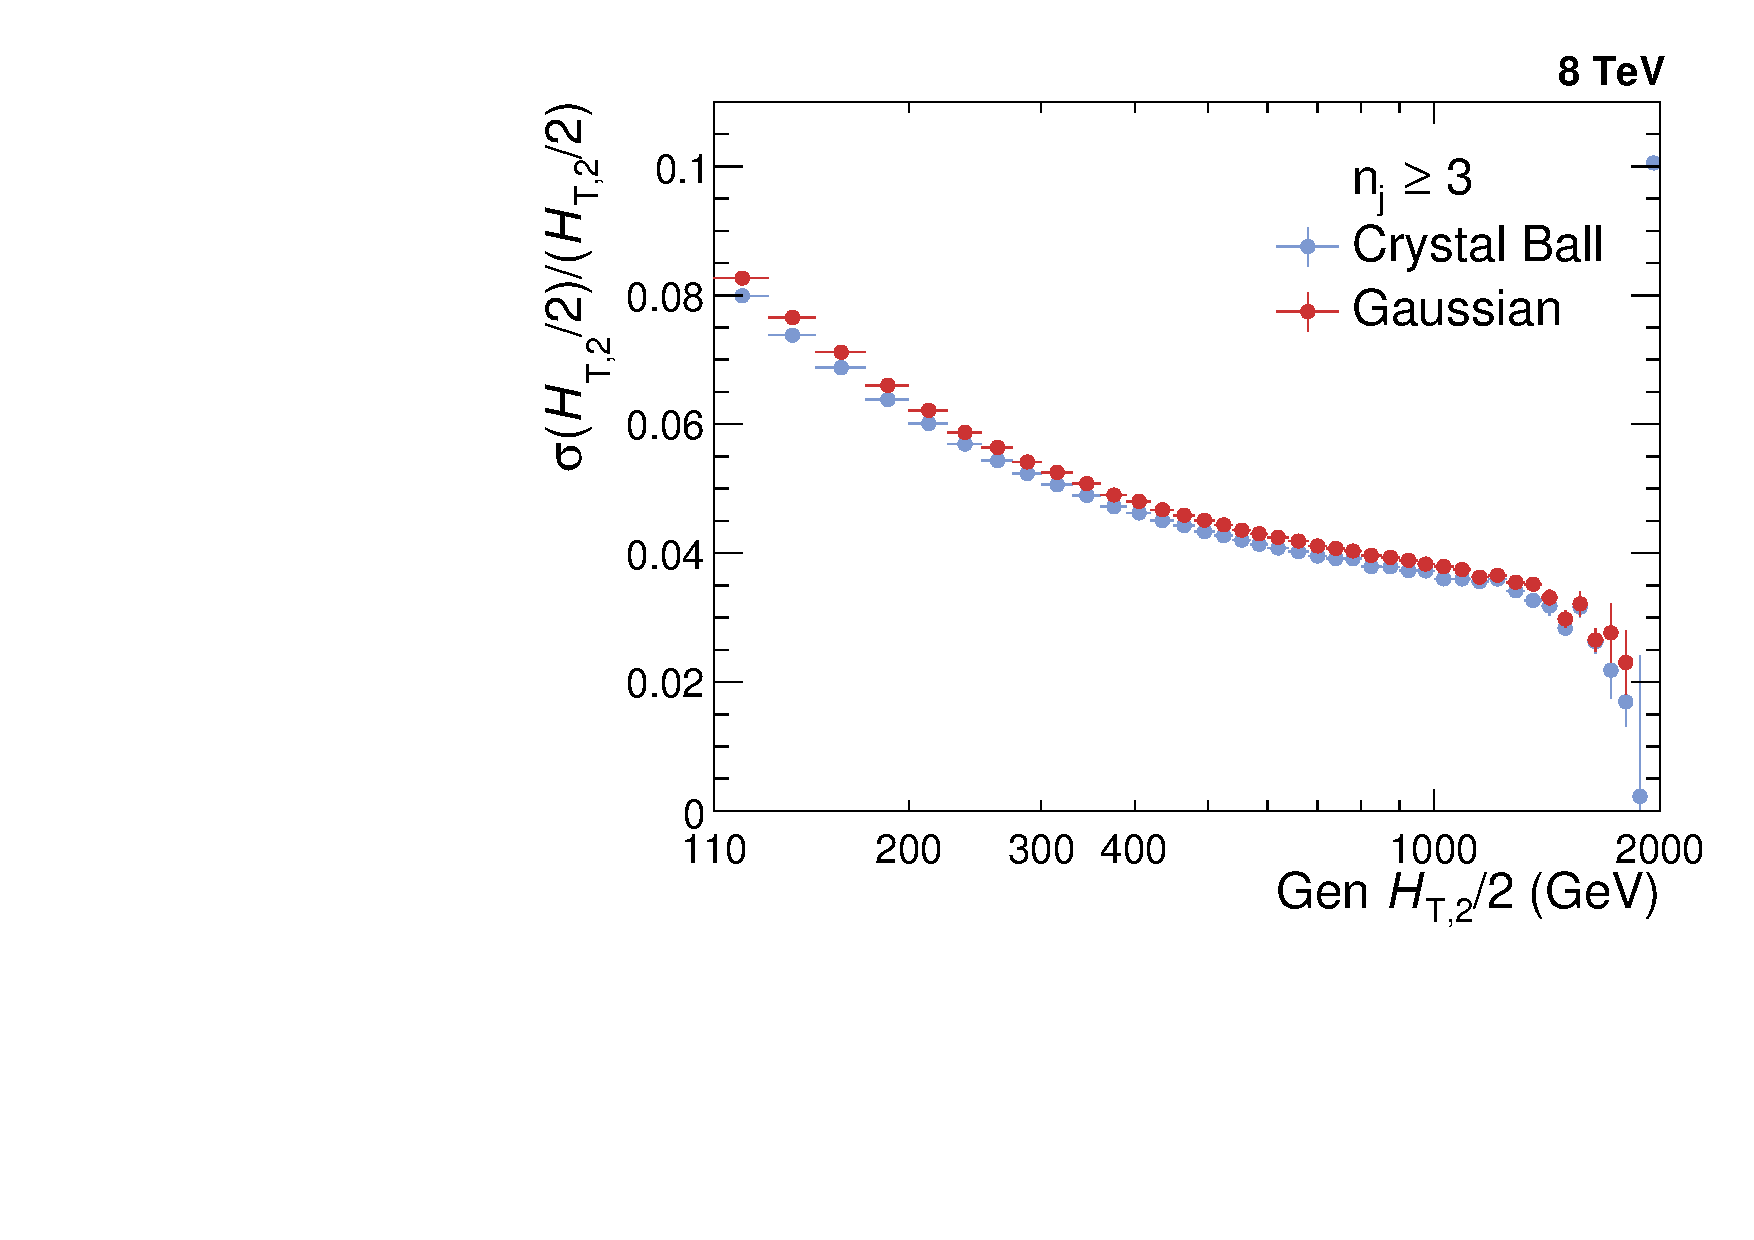
\includegraphics[width=0.5\textwidth]{Plots_HT_2_150/Comparison_Resolution_Crystal_Gauss_3.pdf}
    \caption{Comparison of resolution calculated using Gaussian and Crystal-Ball fit functions for inclusive 2-jet events (left) and for inclusive 3-jet events (right).}
    \label{fig:res_comp}
    
   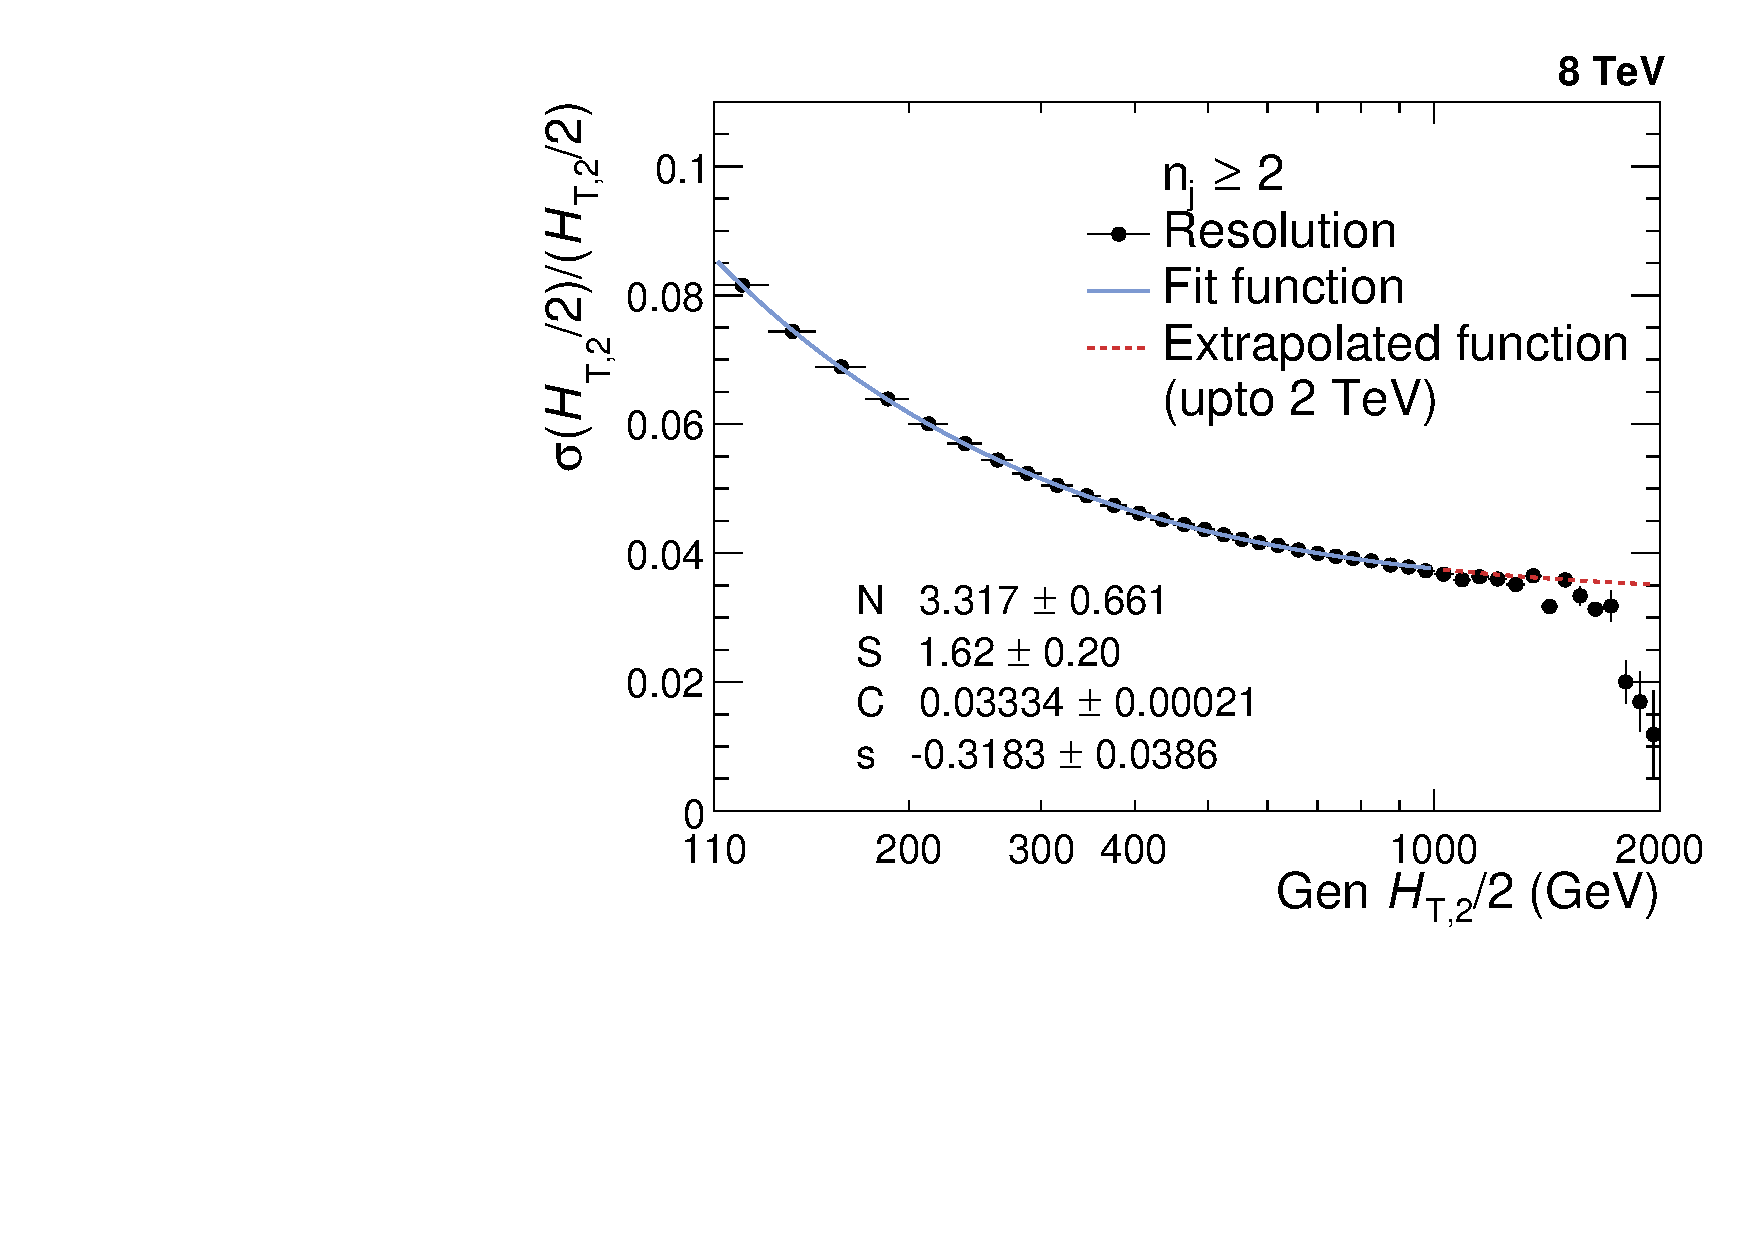
\includegraphics[width=0.5\textwidth]{Plots_HT_2_150/Extrapolate_Sigma_Value_Res_2_crystal_range.pdf}%
    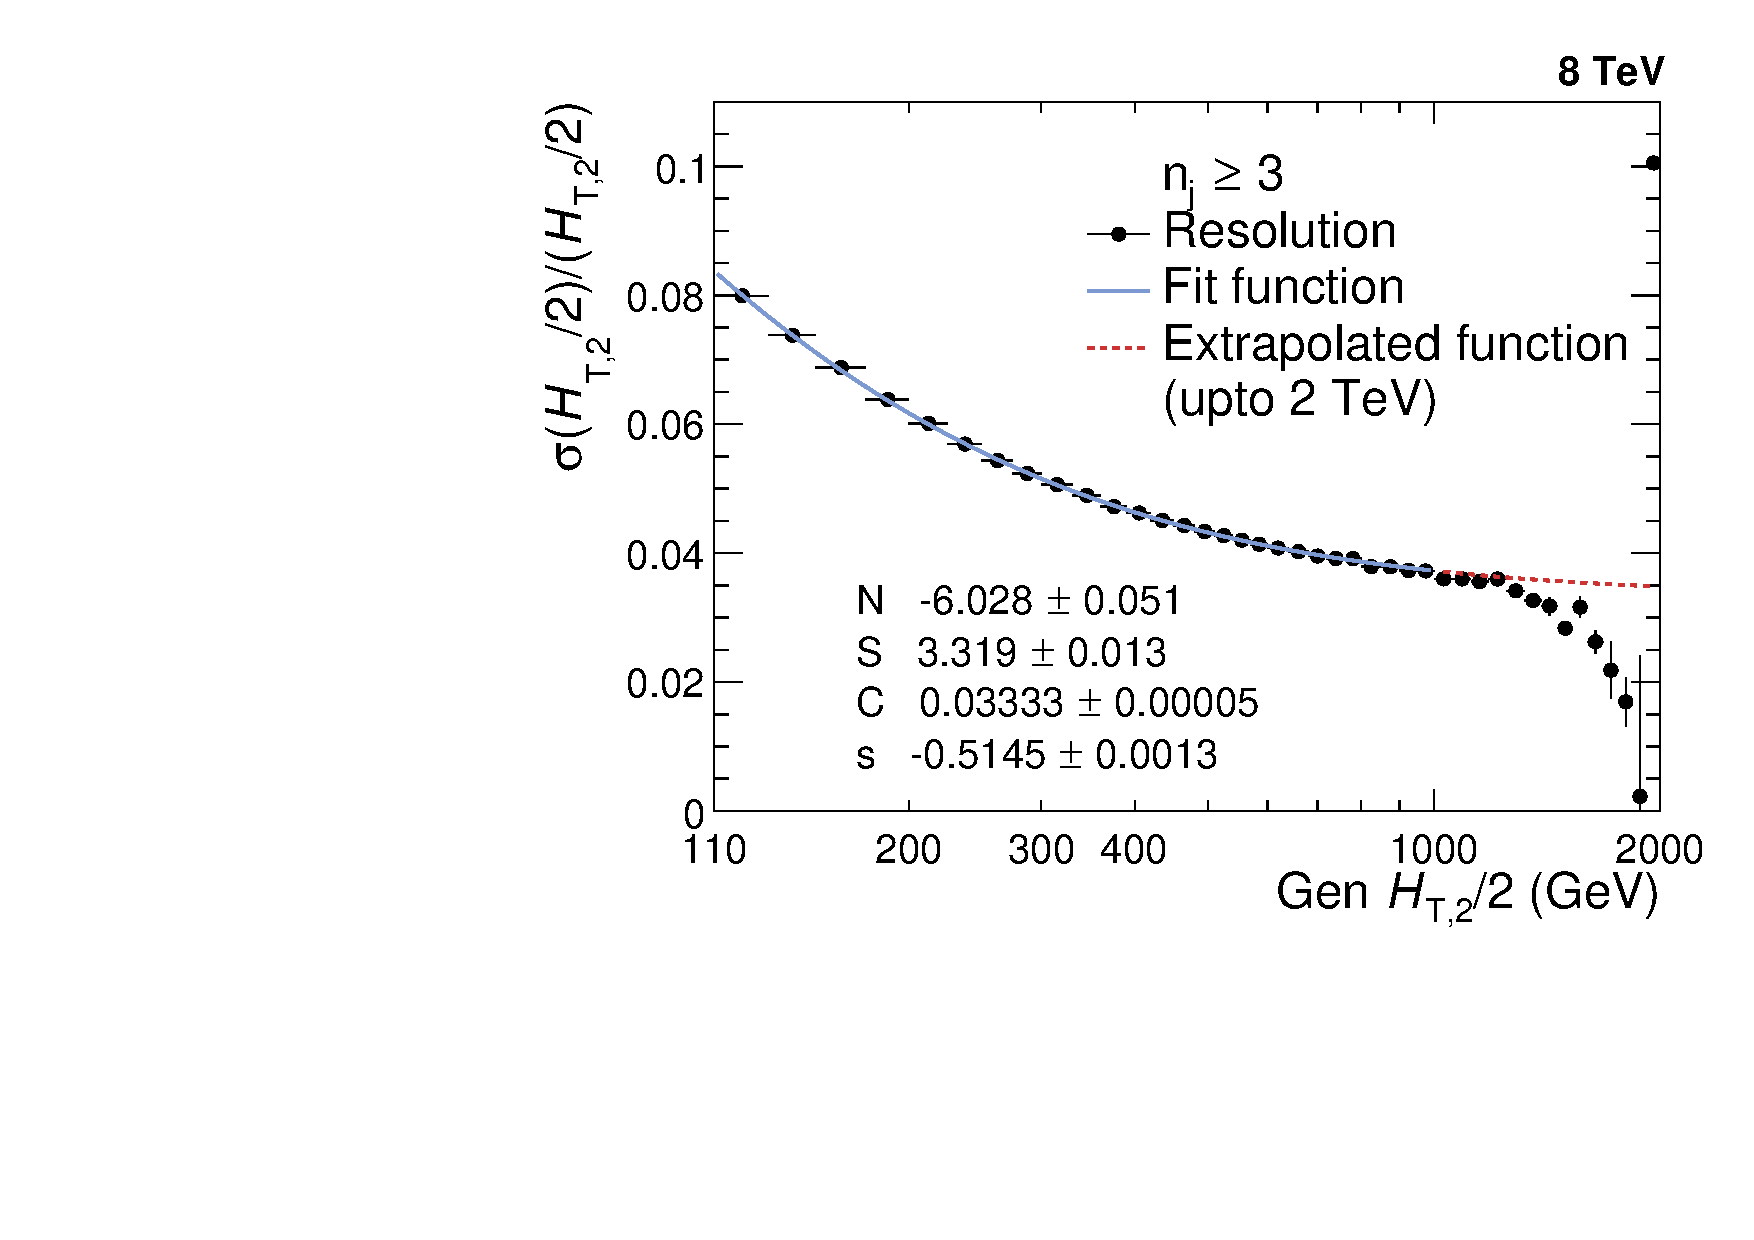
\includegraphics[width=0.5\textwidth]{Plots_HT_2_150/Extrapolate_Sigma_Value_Res_3_crystal.pdf}
    \caption{Resolution as a function of Gen \httwo for inclusive 2-jet events (left) and for inclusive 3-jet events (right).}
    \label{fig:resolution}
  \end{center}
\end{figure}

Figure~\ref{fig:resolution} shows the final relative resolution which is described by a modified version of the NSC formula as mentioned in Equation~\ref{NSC_formula}. Also, the extrapolation of the fit function upto 2 TeV is shown. The formula is based on the usual NSC formula which describes the resolution in terms of noise N, a stochastic component S and a constant term C. Especially in the low \httwo region in which the tracking has a non-negligible influence on the resolution due to the
particle flow algorithm, a slightly better fit is obtained by using the modified resolution formula. Table~\ref{fit_para} gives the 
parameters of the fit for the inclusive 2-jet and inclusive 3-jet events.

\begin{equation}
  \label{NSC_formula}
  \frac{\sigma (x)}{x} = \sqrt{sgn(N) \cdot\frac{N^{2}}{x^{2}}+S^{2}\cdot x^{s-1}+C^{2}} 
\end{equation}

While calculating JER where we are using one large rapidity bin, it has been observed that from Figure~\ref{fig:ratios}, when JER extracted from \blue{simulated MG\plus P6 Reco/MG\plus P6 Gen} is used in toyMC for smearing, it smears the fastNLO too much (\mycolor
{red curve}). The extracted JER also smears MC Gen more as seen from Smeared MG\plus P6 Gen/MG\plus P6 Gen (black dashed curve). When the 30\% reduced JER  is used to smear MG\plus Gen, the  \textcolor{pink}{Smeared MG\plus Gen/MG\plus P6 Gen}, matches with simulated \blue{MG\plus P6
Reco/MG\plus P6 Gen}. Also, toyMC Gen smeared with 30\% reduced  JER, \green{Smeared FastNLO/Gen FastNLO}. So an additional unfolding uncertainty is attributed by comparison to 30\% reduced JER.  

\begin{figure}[!htbp]
  \begin{center}
    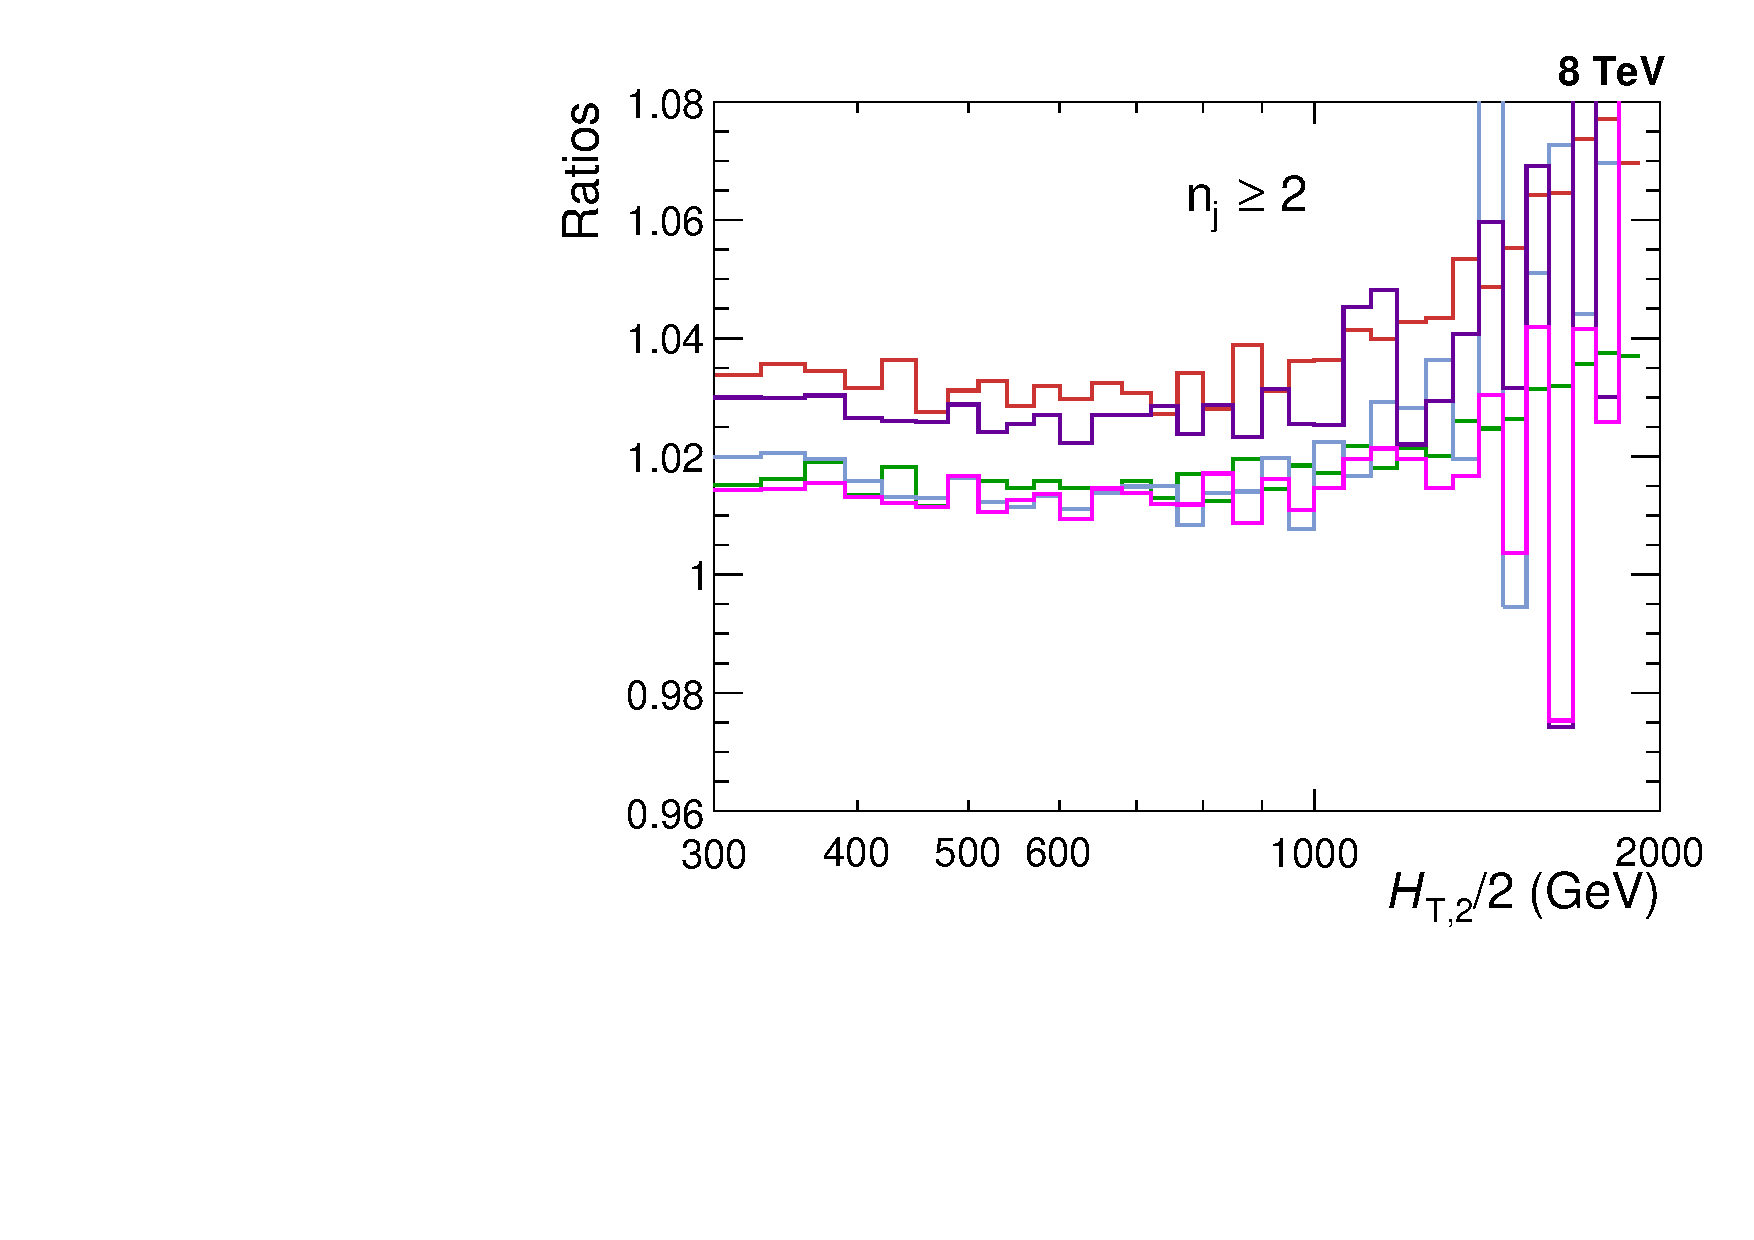
\includegraphics[width=0.5\textwidth]{Plots_HT_2_150/Ratio_all_2_crystal.pdf}%
    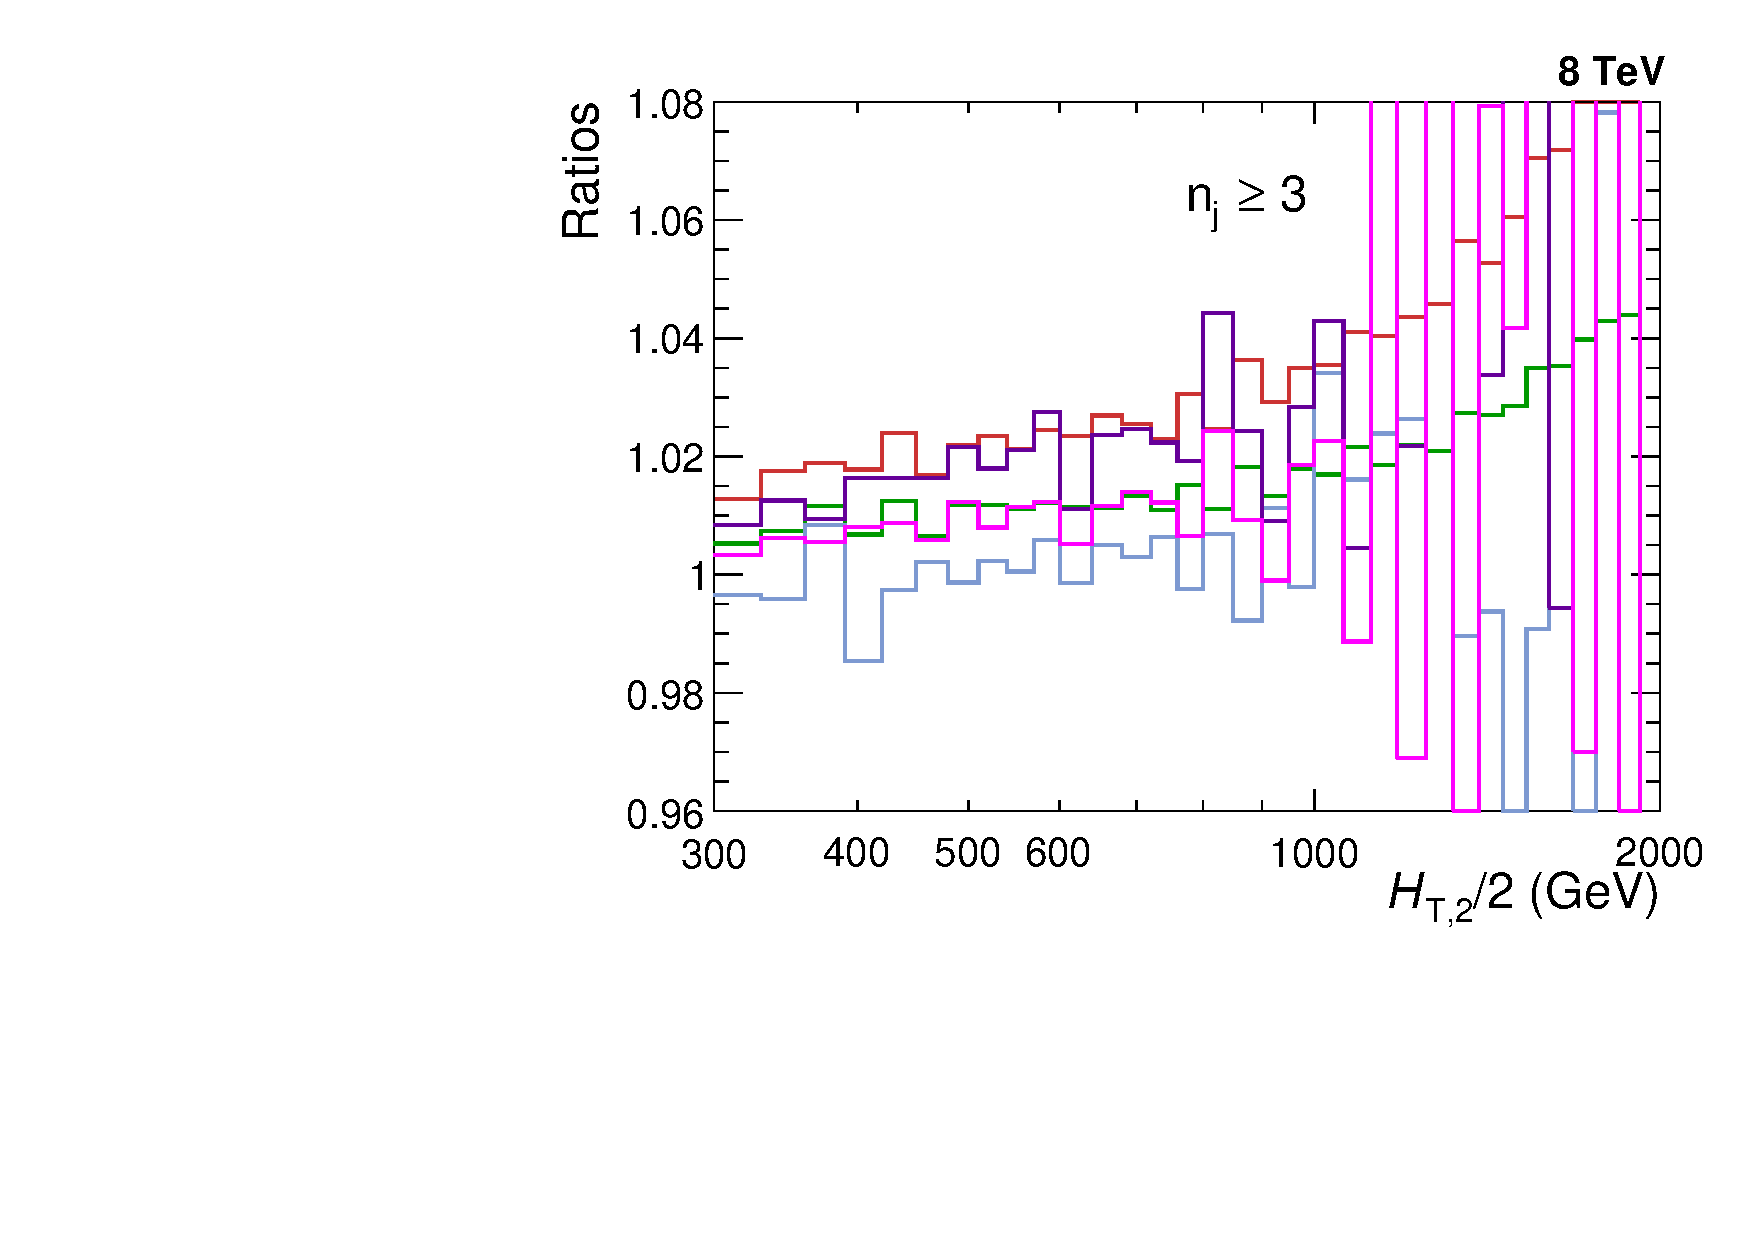
\includegraphics[width=0.5\textwidth]{Plots_HT_2_150/Ratio_all_3_crystal.pdf}\\
    \caption{\blue{Simulated MG\plus P6 Reco/MG\plus P6 Gen} to extract JER, \mycolor {Smeared FastNLO/Gen FastNLO} using extracted JER, Smeared MG\plus P6 Gen/MG\plus P6 Gen using extracted JER,  \textcolor{pink} {smeared MG\plus P6 Gen/MG\plus P6 Gen} using 30\% reduced extracted JER, \green {Smeared FastNLO/Gen FastNLO} using 30\% reduced extracted JER; for inclusive 2-jet (left) and inclusive 3-jet events (right).}
    \label{fig:ratios}
  \end{center}
\end{figure}

\begin{table}[!htbp]
  \centering
  \caption{The fit parameters of the resolution for inclusive 2-jet and inclusive 3-jet events.}
  \label{fit_para}
  \vspace{2mm}
  \begin{tabular}{ccccc}
    \hline \hline

    &    N    &  S   &    C   &    s   \rbtrr \\ \hline
    Inclusive 2-jet  & ~3.32 & 1.62 & 0.0333 & -0.318  \rbtrr \\
    Inclusive 3-jet  & -6.03 & 3.32 & 0.0333 & -0.515  \rbtrr \\
    \hline \hline
    
  \end{tabular}
\end{table}

\subsection{Unfolding}
\label{sec:unfolding}
One of the main goal in the experimental measurement is to do the comparison between data and theory predictions or with the results from 
other experiments. But the finite detector resolution and the steeply falling jet \pt spectrum distorts the physical quantities. As a 
result, the measured observables are different from the corresponding true values. Each \pt bin content contains the migrated events from 
neighbouring bins along with the original events. So an unfolding process of the data for detector effects should be followed. Unfolding 
uses a response matrix that maps the true distribution onto the measured one. The response matrix is usually derived from simulated Monte 
Carlo (MC) samples (eg. \PYTHIAS tune Z2 MC), which uses as input the true distribution from MC and introduces the smearing effects by 
taking into account the detector resolution. Then this response matrix is used to unfold the measured data spectrum. There are several 
drawbacks of constructing response matrix from the MC as MC is not perfectly calibrated. Also dealing with the systematic uncertainties is 
practically impossible with this technique.

However, there is an indirect way of constructing the response matrix which 
uses a custom Toy Monte Carlo by utilizing NLO prediction whose 
details are given in section~\ref{sec:funcs}. The particle level \httwo spectrum is 
obtained from the falling fitted function used to fit the theoretically 
predicted \httwo spectrum.  The reconstructed level \httwo spectrum is 
obtained by smearing the particle level \httwo spectrum with the jet energy 
resolution (JER) parameters.  

In this analysis, the measured cross sections are corrected for detector 
smearing effects and unfolded to stable particle level and then the ratio 
\ratio is constructed. We have used the iterative D'Agostini Bayesian method 
with four iterations~\cite{D'Agostini:1994zf}, implemented in the RooUnfold 
software package~\cite{Adye:2011gm}. 

\subsubsection{Response matrices}
\label{sec:funcs}
The NLO spectrum of differential cross section is fitted with the following two different functions :  

\begin{itemize}
\item {\bf Function I : }
  %\end{itemize} 

  \begin{equation}
    \label{eq:func1}
    f(p_{T}) = N[x_{T}]^{-a}[1-x_{T}]^{b} \times exp[-c/x_{T}]
  \end{equation}
  where N is normalization factor and a, b, c are fit parameters.\\

  This function is derived from the below function from \textbf{Phys.Rev.Lett. 107, 132001 (2011)}\\
  \begin{center}
    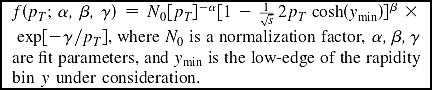
\includegraphics[scale = 0.65]{Plots_HT_2_150/Formula.png} 
  \end{center}
  using 
  \begin{equation}
    \alpha = a,~~\beta = b,~~\gamma = c*\sqrt{s}/2, \\
    x_{T} = \frac{2*p_{T}*cosh(y_{min})}{\sqrt{s}} = \frac{2*p_{T}}{\sqrt{s}}
  \end{equation}
  where transverse scaling variable $x_{T}$ corresponds to the proton fractional momentum x for dijets with rapidity y=0, $\sqrt{s}$ = 8000 GeV and $y_{min}$ is low-edge of the rapidity bin y under consideration (Here $y_{min}$ is taken equal to 0) \\ 

\item {\bf Function II : }

  \begin{equation}
    \label{eq:func2}
    f(H_{T,2}/2) = A_{0}\Big(1-\frac{H_{T,2}/2}{A_{6}}\Big)^{A_{7}} \times 10^{F(x)}, \rm where ~~~{F(x) = \sum\limits_{i=1}^5 A_{i}\Big(log\big(\frac{x}{A_{6}}\big)\Big)^{i}}
  \end{equation}

  where the parameter $A_{6}$ is fixed to $\frac{\sqrt{s}}{2cosh(y_{min})}$, where $\sqrt{s}$ = 8000 GeV and $y_{min}$ is 
  the minimum rapidity. The other parameters are derived from the fitting.
\end{itemize}

\begin{figure}[!htbp]
  \begin{center}
    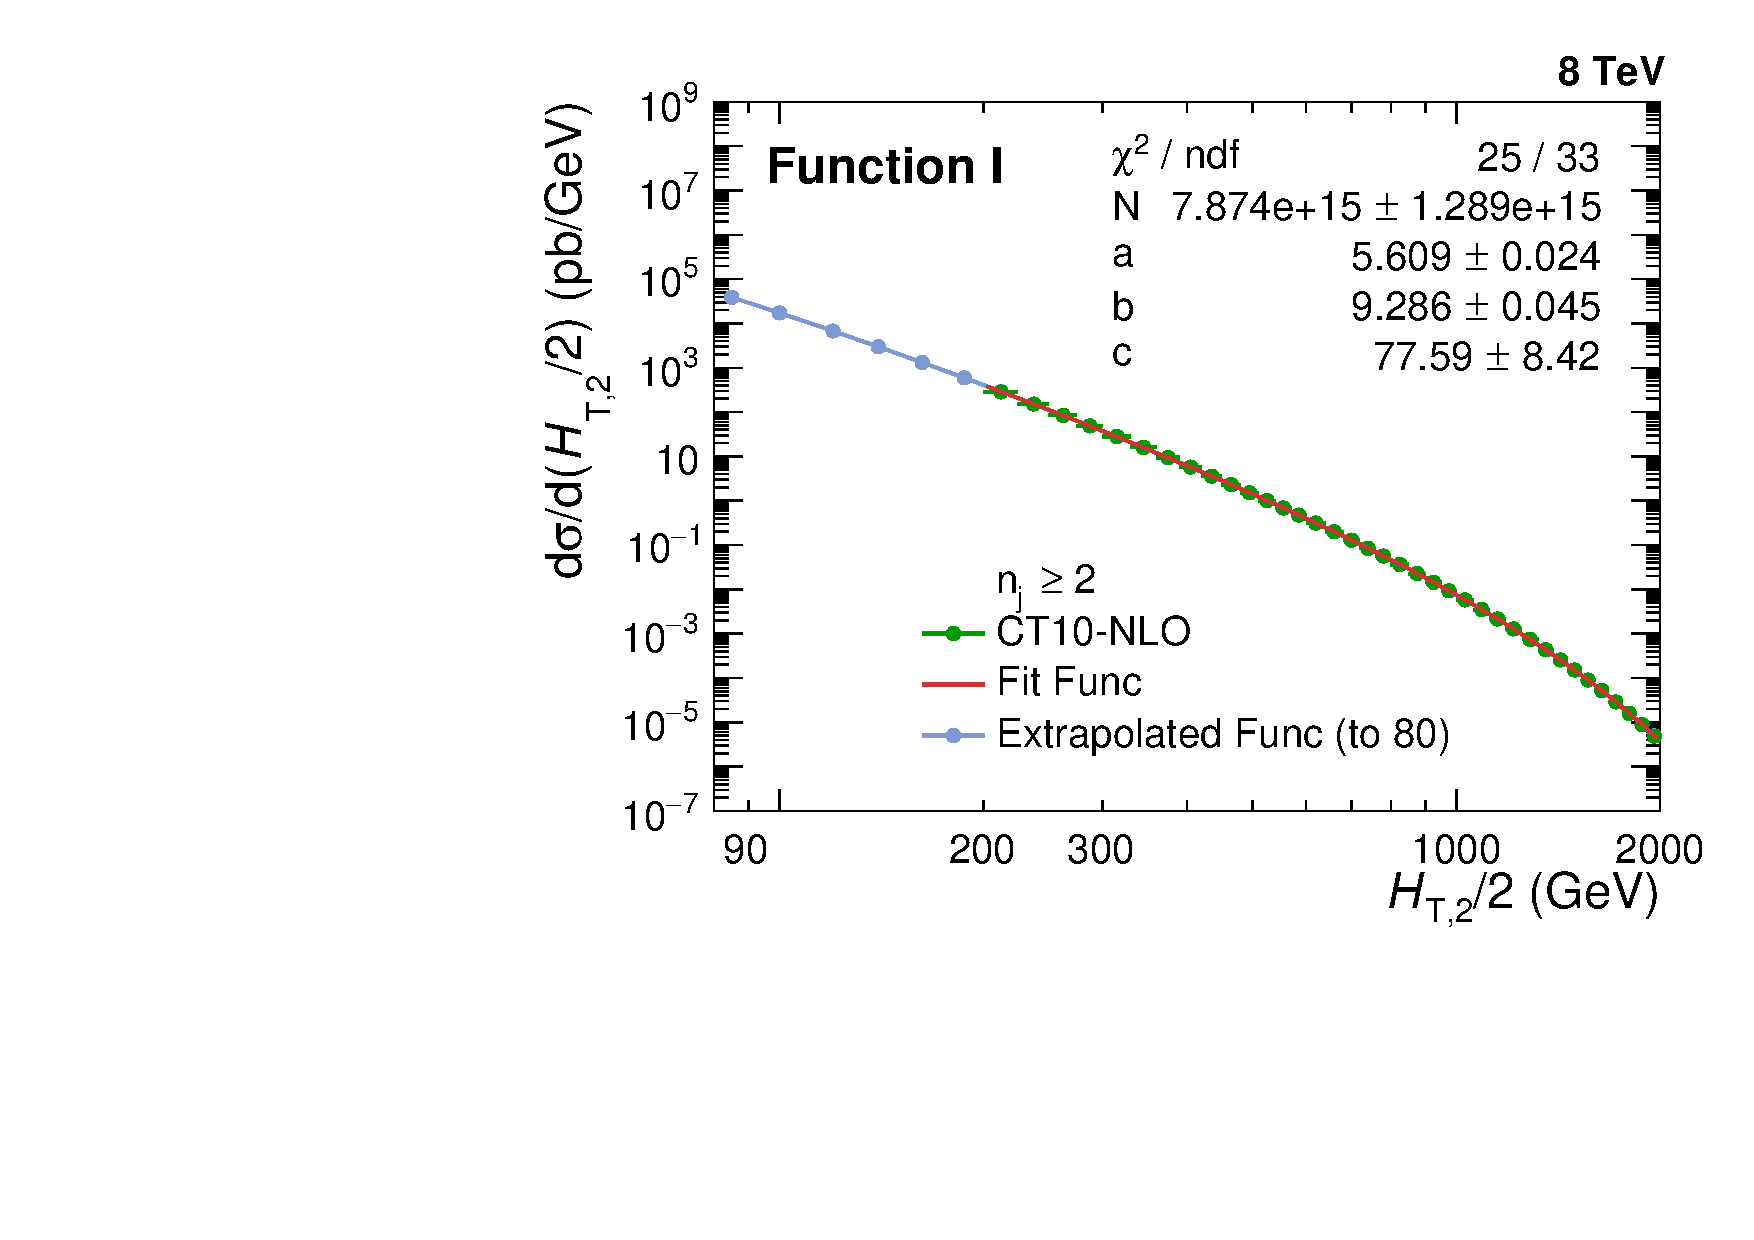
\includegraphics[width=0.5\textwidth]{Plots_HT_2_150/Extrapolate_Theory_2_HT_2_150_funcI.pdf}%
    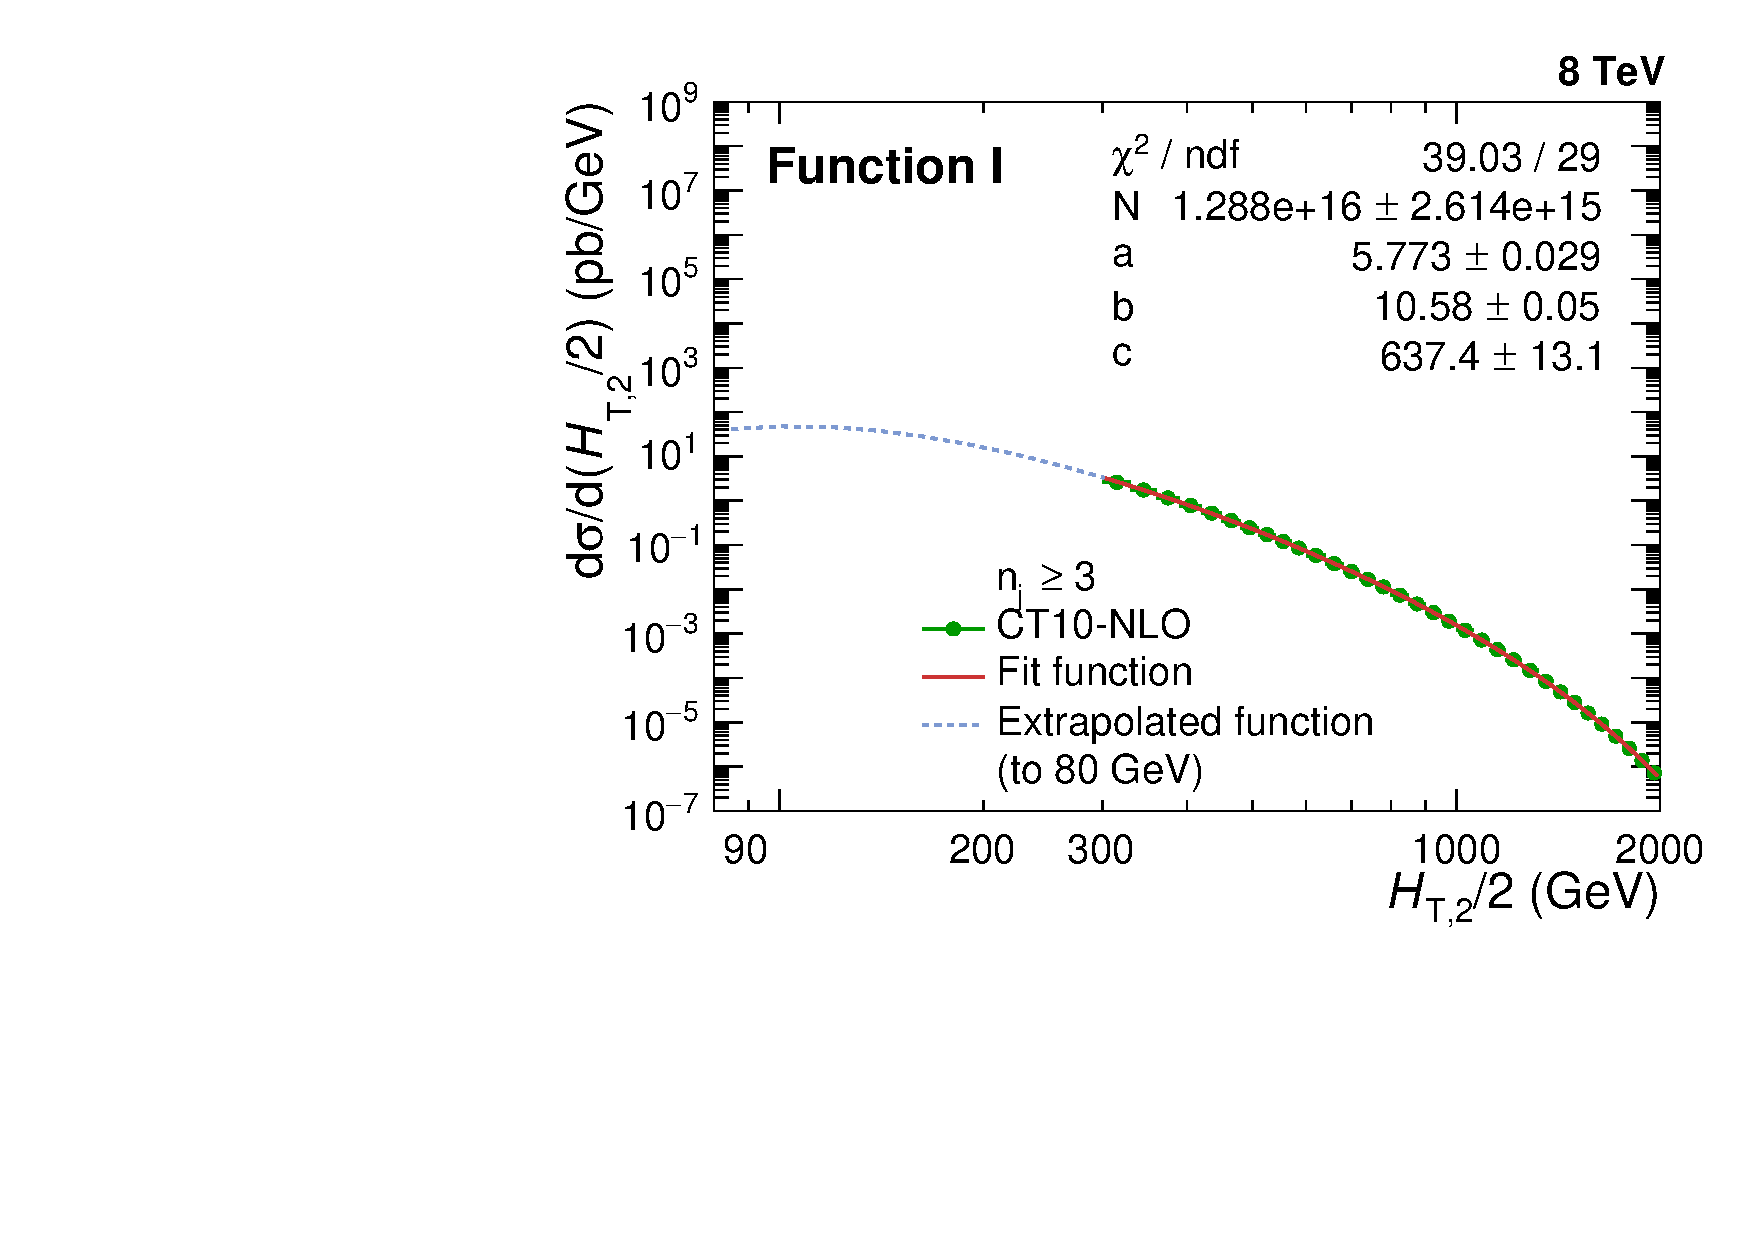
\includegraphics[width=0.5\textwidth]{Plots_HT_2_150/Extrapolate_Theory_3_HT_2_150_funcI.pdf}\\
    \vspace{5mm}
    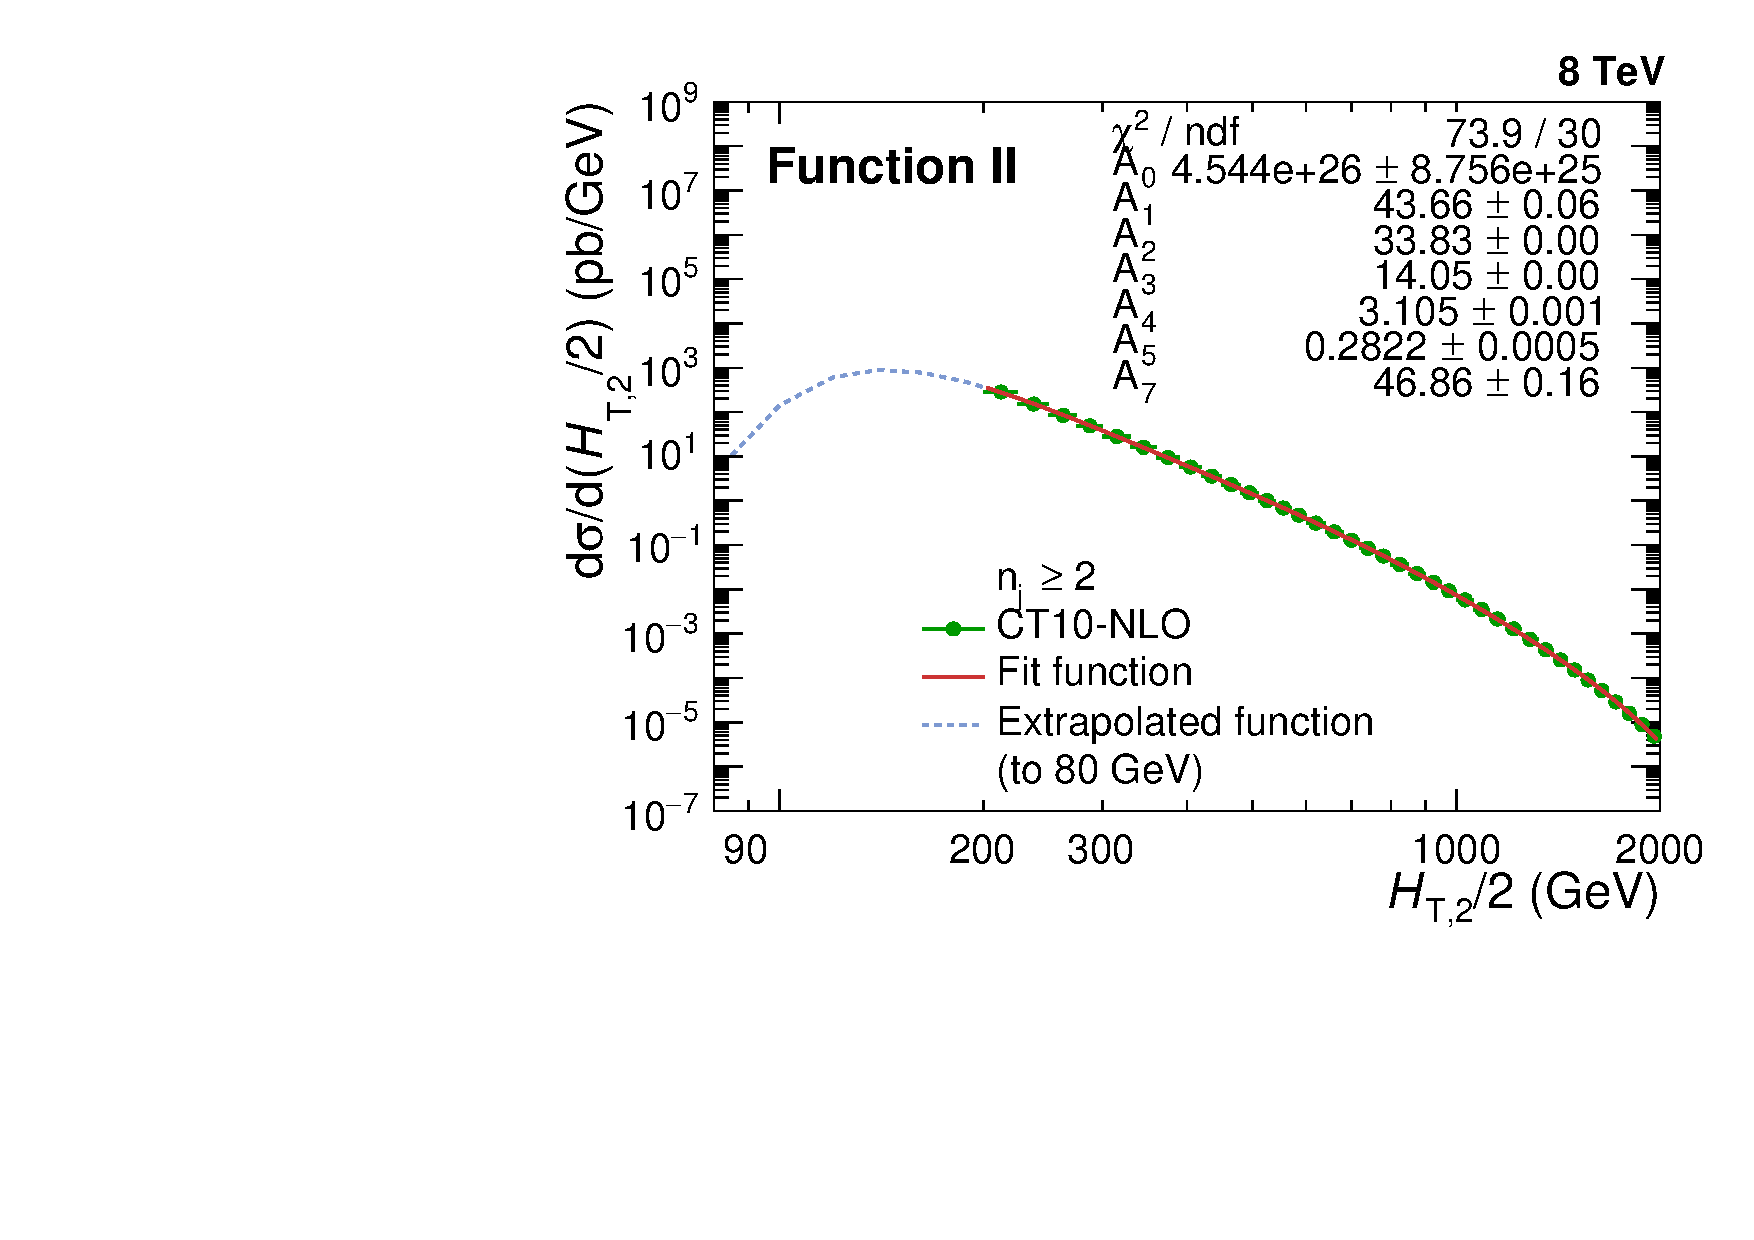
\includegraphics[width=0.5\textwidth]{Plots_HT_2_150/Extrapolate_Theory_2_HT_2_150_funcII.pdf}%
    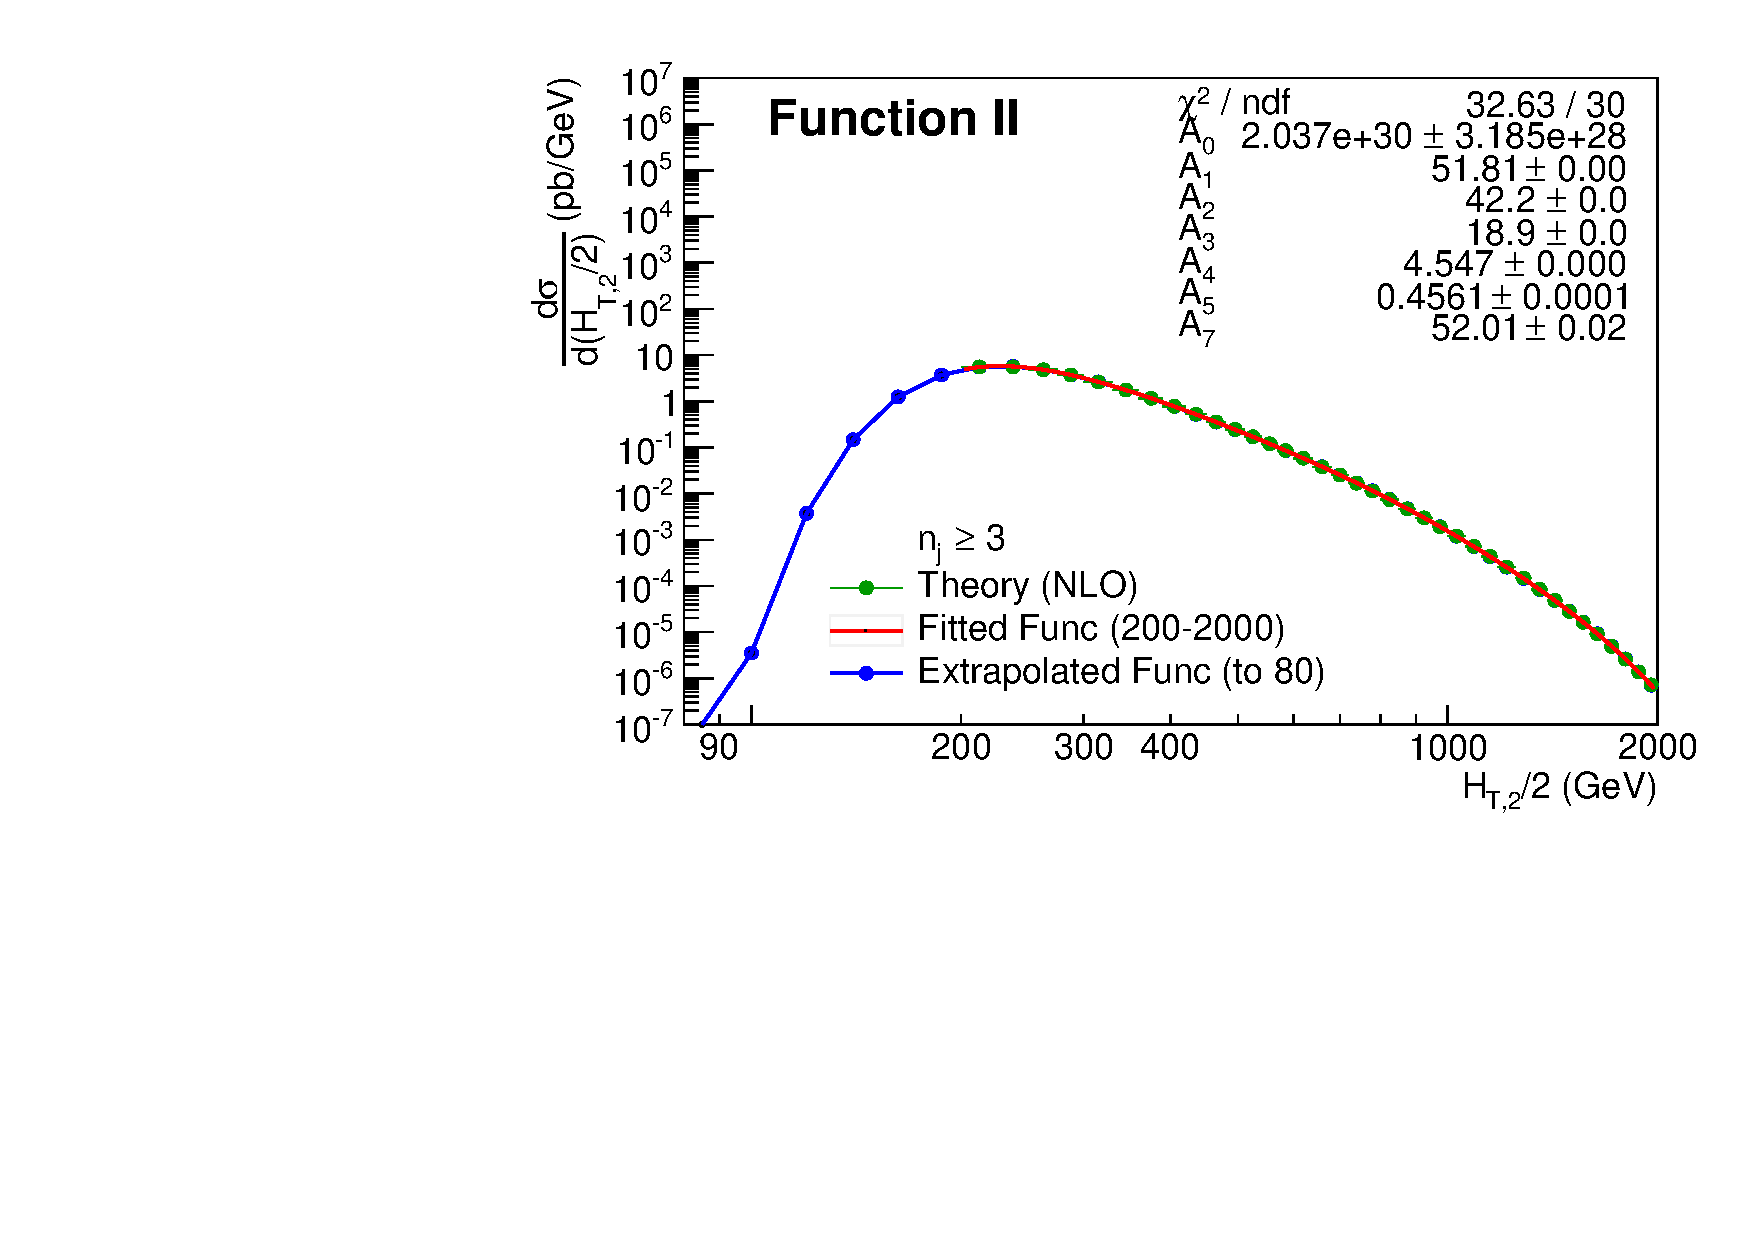
\includegraphics[width=0.5\textwidth]{Plots_HT_2_150/Extrapolate_Theory_3_HT_2_150_funcII.pdf}\\
    \caption{Fitted NLO spectrum of differential cross section as a function of \httwo using Function I (top) and using Function II (bottom) : for inclusive 2-jet events (left) and for inclusive 3-jet events (right).}
    \label{fig:fit}
  \end{center}
\end{figure}

Figure~\ref{fig:fit} shows the fitted NLO spectrum of differential cross section as a function of \httwo using Function I (top) and using 
Function II (bottom) : for inclusive 2-jet events (left) and for inclusive 3-jet events (right). Function I is used primarily to 
generate response matrices and perform the closure tests and Function II is used as an alternative function to calculate unfolding 
uncertainty, described in section~\ref{sec:unfolding_unc}. To include the migration to lower bins, the fitted functions are extrapolated to 
the lower \httwo values.

\begin{figure}[!htbp]
  \begin{center}
    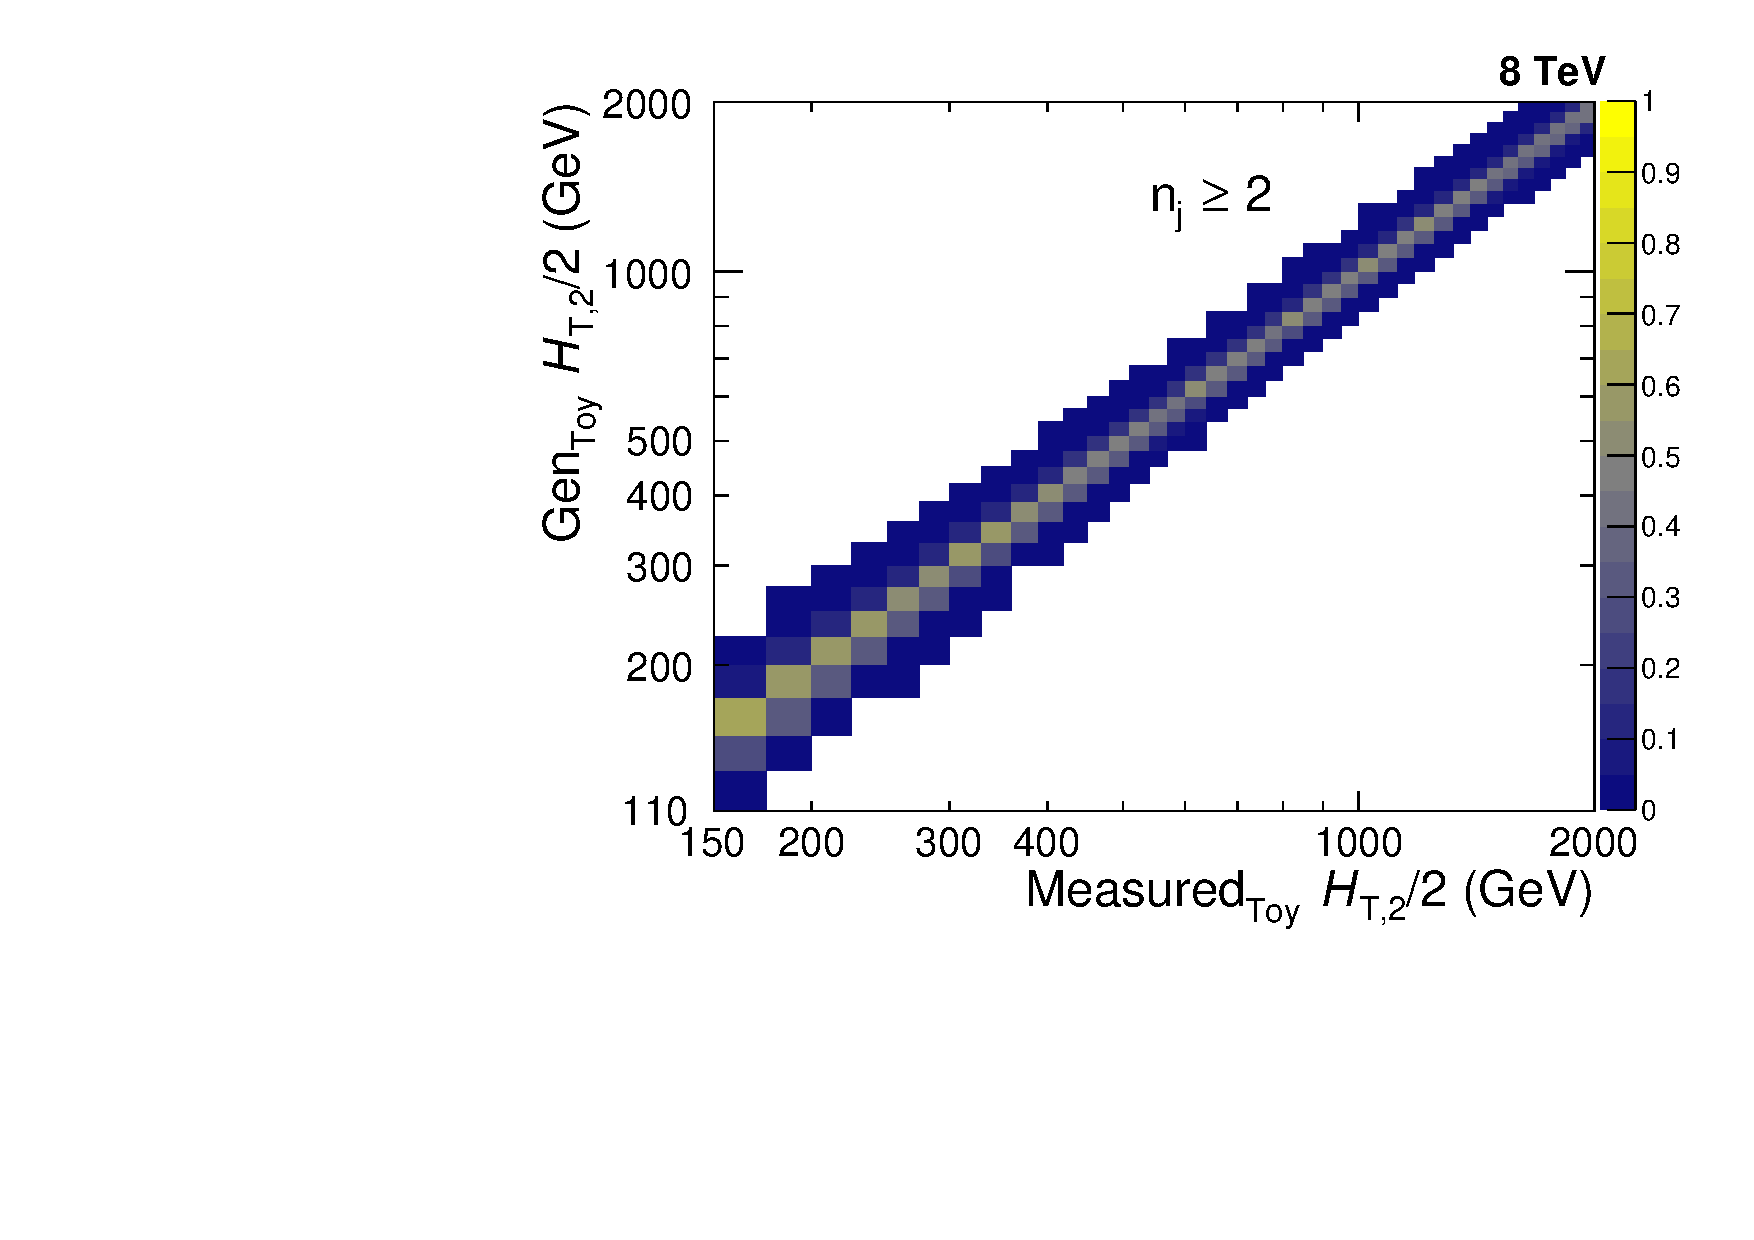
\includegraphics[width=0.45\textwidth]{Plots_HT_2_150/Normalized_Response_Matrix_NLO_2_range_column.pdf}%
    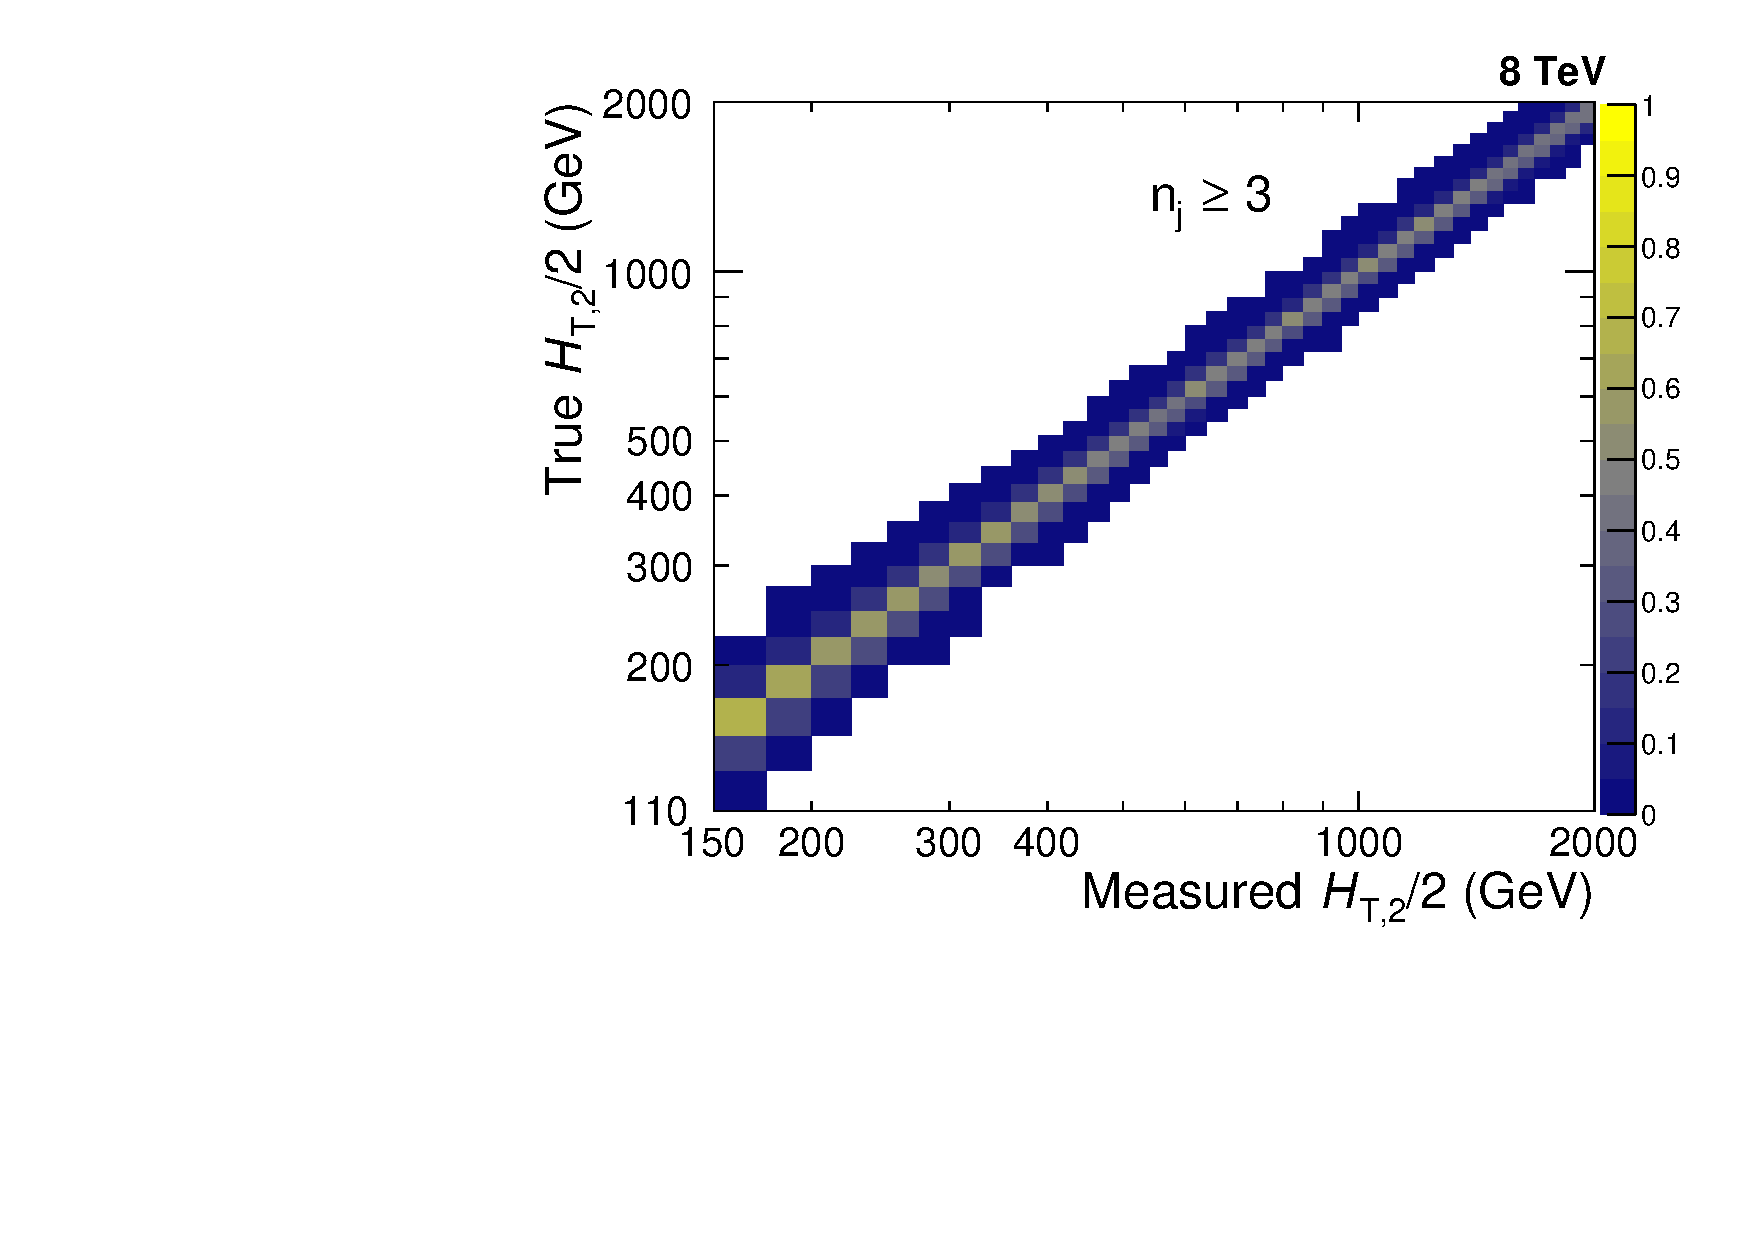
\includegraphics[width=0.45\textwidth]{Plots_HT_2_150/Normalized_Response_Matrix_NLO_3_column.pdf} 
    \caption{The response matrices derived using the Toy MC for inclusive 2-jet (left) and inclusive 3-jet events (right).}
    \label{fig:response_NLO}
  %\end{center}
%\end{figure}

%\begin{figure}[!htbp]
%  \begin{center}
    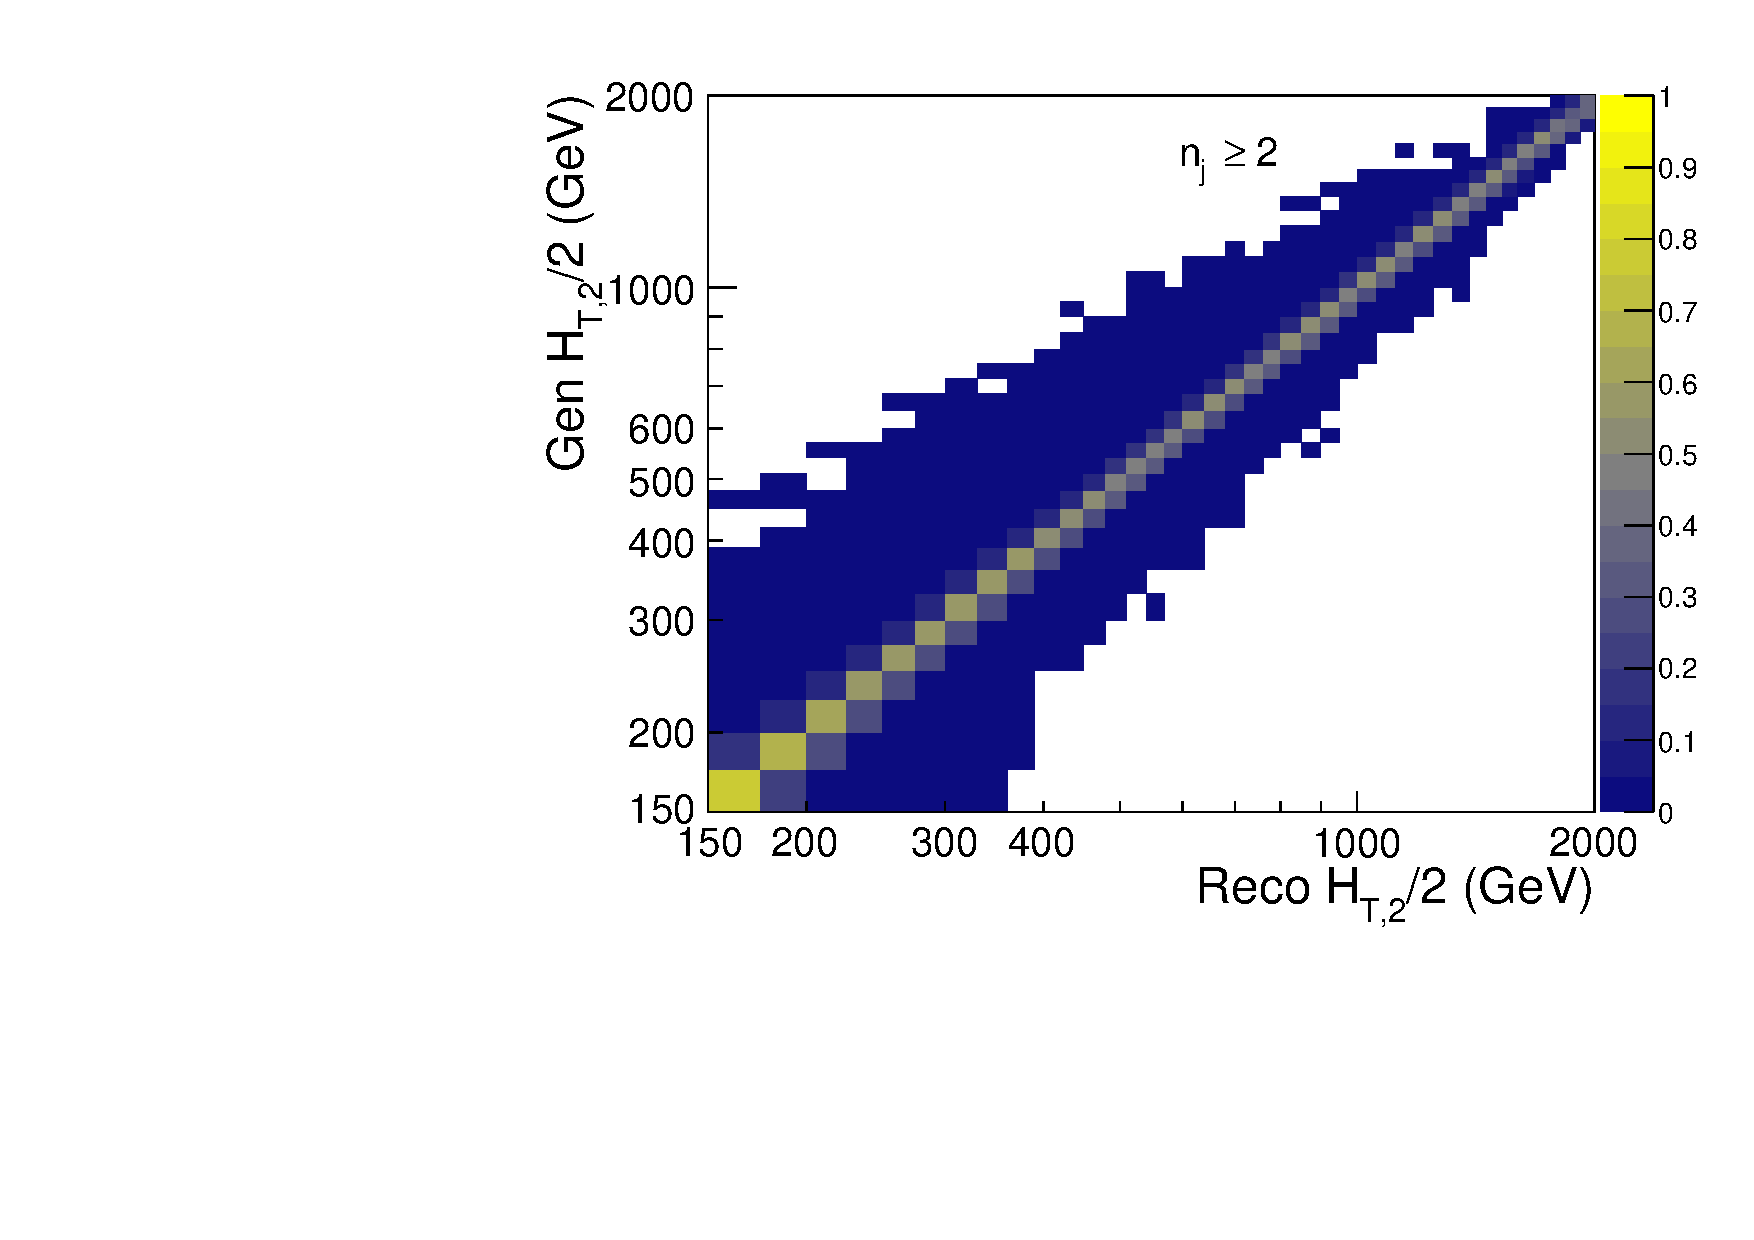
\includegraphics[width=0.45\textwidth]{Plots_HT_2_150/Normalized_Response_Matrix_Madgraph_2_HT_2_150.pdf}%
    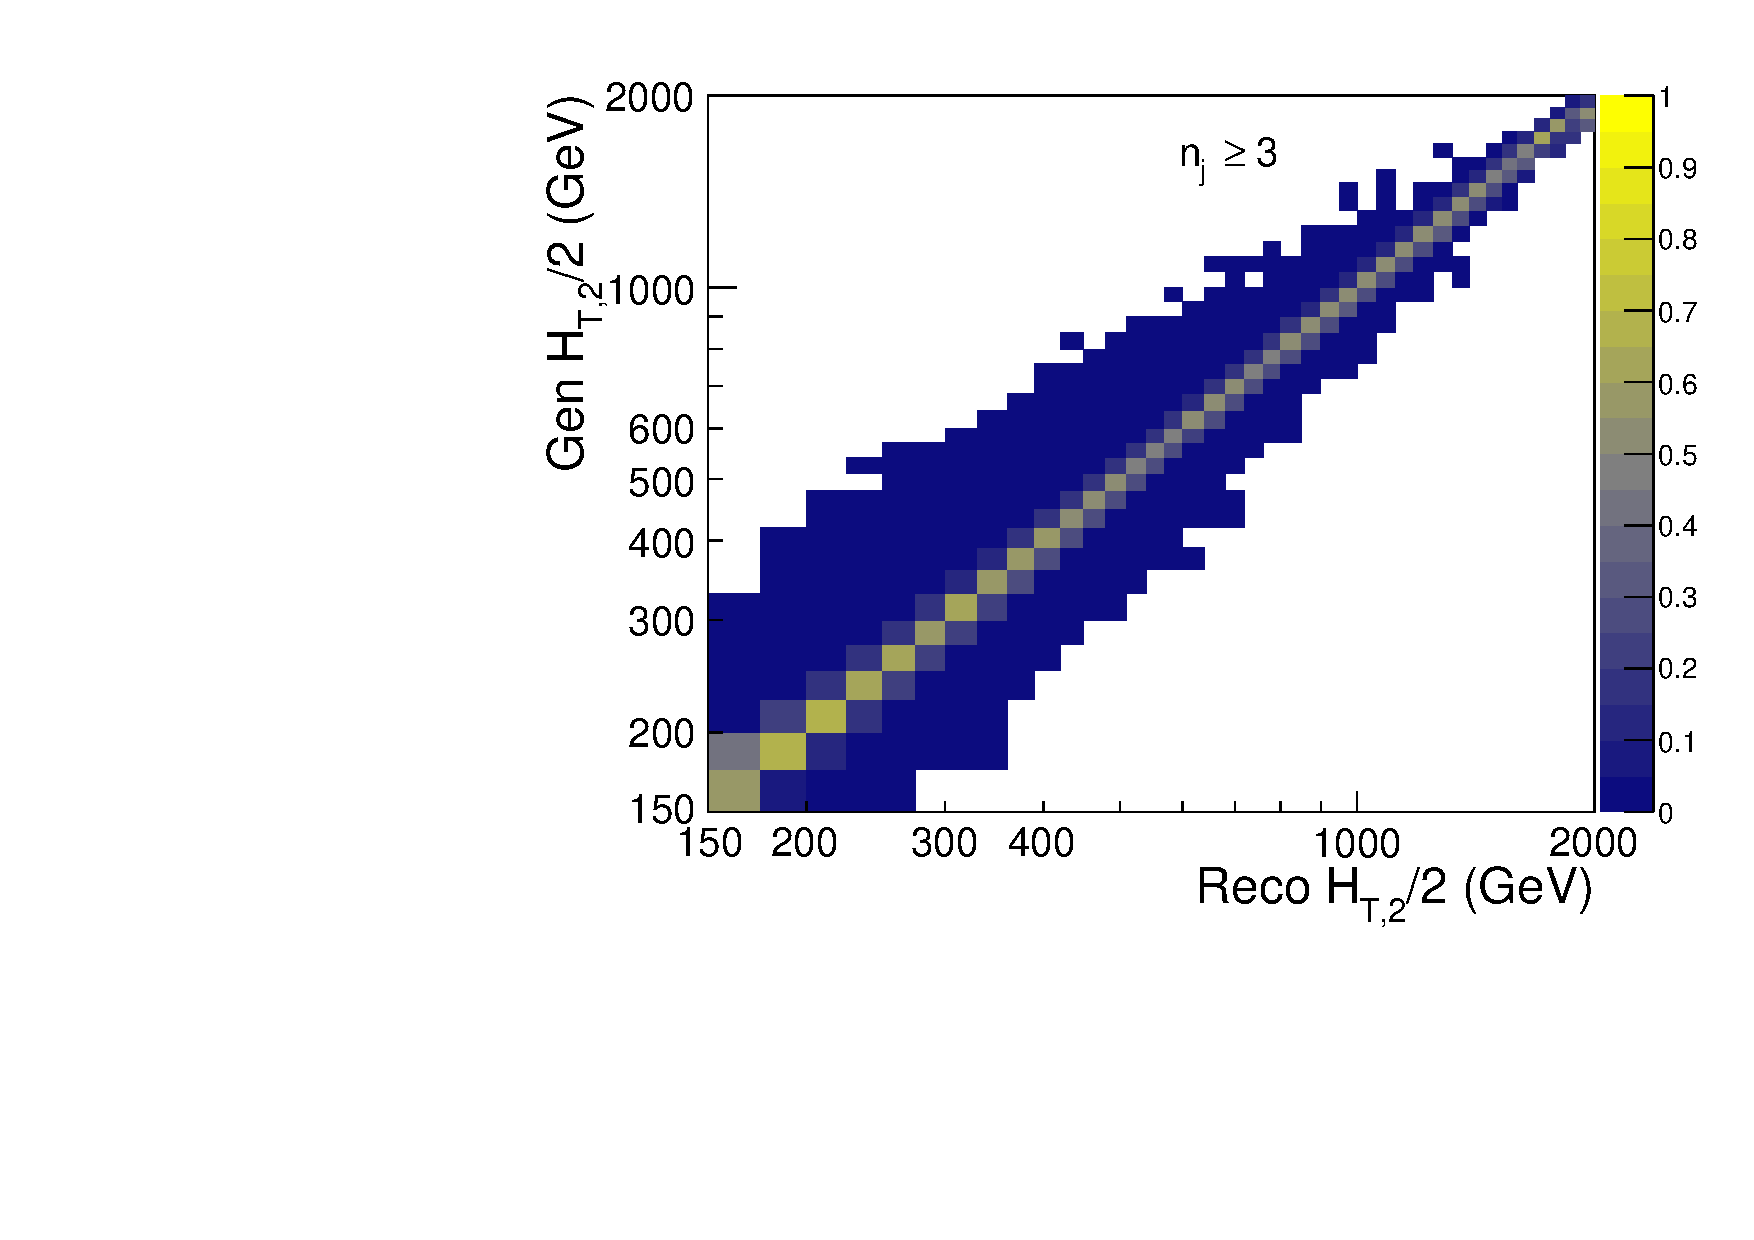
\includegraphics[width=0.45\textwidth]{Plots_HT_2_150/Normalized_Response_Matrix_Madgraph_3_HT_2_150.pdf}\\
    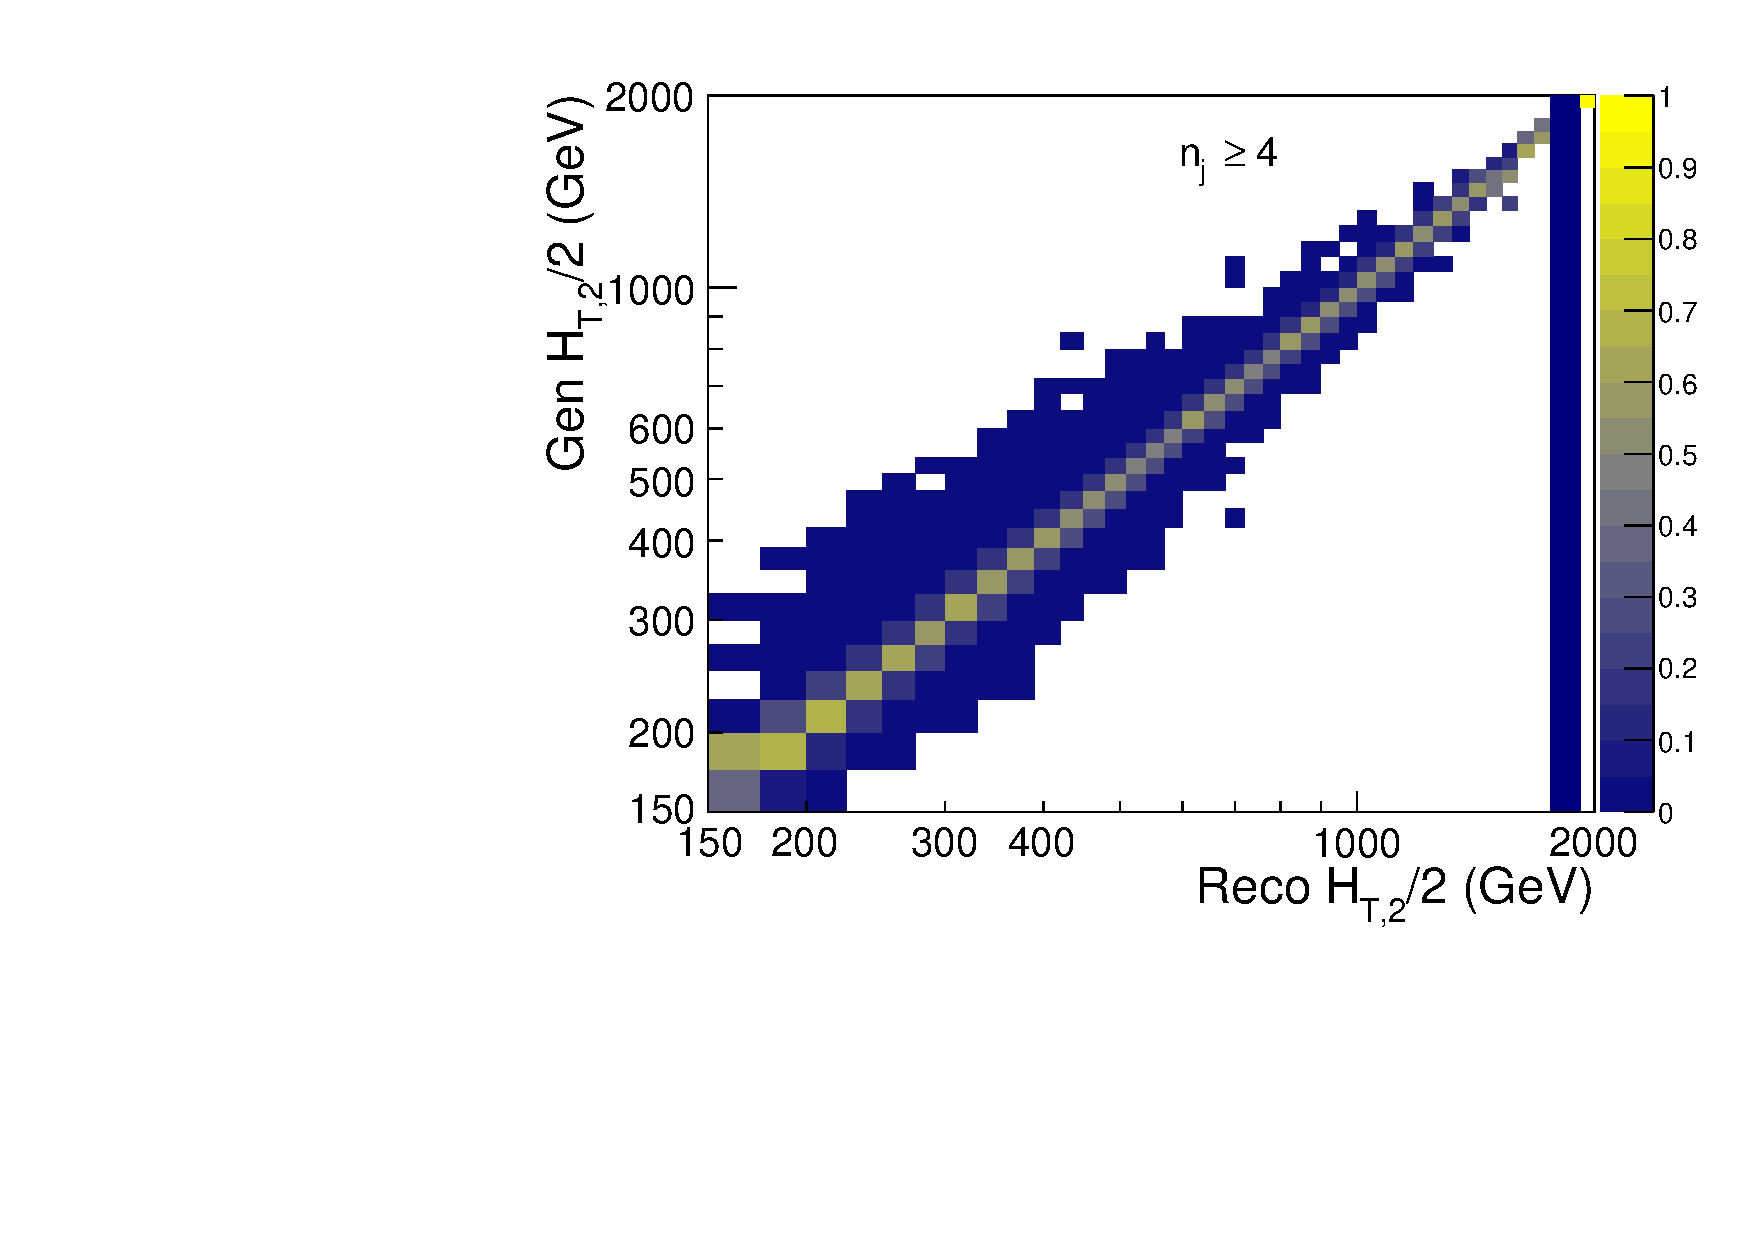
\includegraphics[width=0.45\textwidth]{Plots_HT_2_150/Normalized_Response_Matrix_Madgraph_4_HT_2_150.pdf} 
    \caption{The response matrices constructed from \MadGraphF + \PYTHIAS MC inclusive 2-jet (top left), inclusive 3-jet events (top right) and inclusive 4-jet events (bottom).}
    \label{fig:response_MC}
  \end{center}
\end{figure}

A flat \httwo spectrum is generated and the fit parameters obtained from the NLO spectrum provides weights to the flat spectrum. A total of 
ten million events are generated (in \httwo range 80-2000). These generated values are smeared with a Gaussian function, where $\sigma$ of 
the Gaussian is determined from the relative resolution parametrization as a function of \httwo calculated from NSC formula mentioned in 
equation~\ref{NSC_formula}. The parameters N, S, C used for smearing are taken from Table~\ref{fit_para}.

These generated and smeared values are used to fill the response matrices by using the RooUnfold package. Figure~\ref{fig:response_NLO} 
shows the response matrices derived using the Toy MC for inclusive 2-jet (left) and inclusive 3-jet events (right). The matrices 
are normalized to the number of events in each column. The response matrices are diagonal with small off-diagonal migrations between close-
by \httwo bins.

Also, the response matrices are constructed from \MadGraphF + \PYTHIAS MC using the distributions from PFJets (Jets based on individual 
particles reconstructed by the Particle Flow Algorithm) and GenJets (Jets found by applying a jet algorithm on MC stable particles which are
produced at the end of the hadronization stage). Figure~\ref{fig:response_MC} shows the response matrices constructed from \MadGraphF + 
\PYTHIAS MC for inclusive 2-jet (top left), inclusive 3-jet events (top right) and inclusive 4-jet events (bottom).

\subsubsection{Closure test}
First we unfold the smeared spectrum obtained from Toy MC, using the constructed response matrices shown in Figure~\ref{fig:response_NLO} 
to check how good the unfolding procedure is working. Figure~\ref{fig:unfolded_smeared} shows that after unfolding, the smeared spectrum 
matches exactly with the randomly generated spectrum as the ratio of these distributions is perfectly flat at one for both inclusive 2-jet 
(left) as well as inclusive 3-jet events (right).

Also we unfold the distribution from PFJets obtained from \MadGraphF + \PYTHIAS MC using the constructed response matrices shown in 
Figure~\ref{fig:response_MC}. Figure~\ref{fig:unfolded_reco} shows that after unfolding, the spectrum from PFJets matches exactly with that 
from GenJets as expected.

Also we unfold the distribution from PFJets obtained from \MadGraphF + \PYTHIAS MC with the toyMC response matrices shown in 
Figure~\ref{fig:response_NLO}. While performing this closure test, it has been observed that when 30\% reduced JER is used to unfold \MadGraphF + \PYTHIAS Reco MC, a good closure is obtained as seen in  Figure~\ref{fig:unfolded_reco_NLO}.

\begin{figure}[!htp]
  \begin{center}
    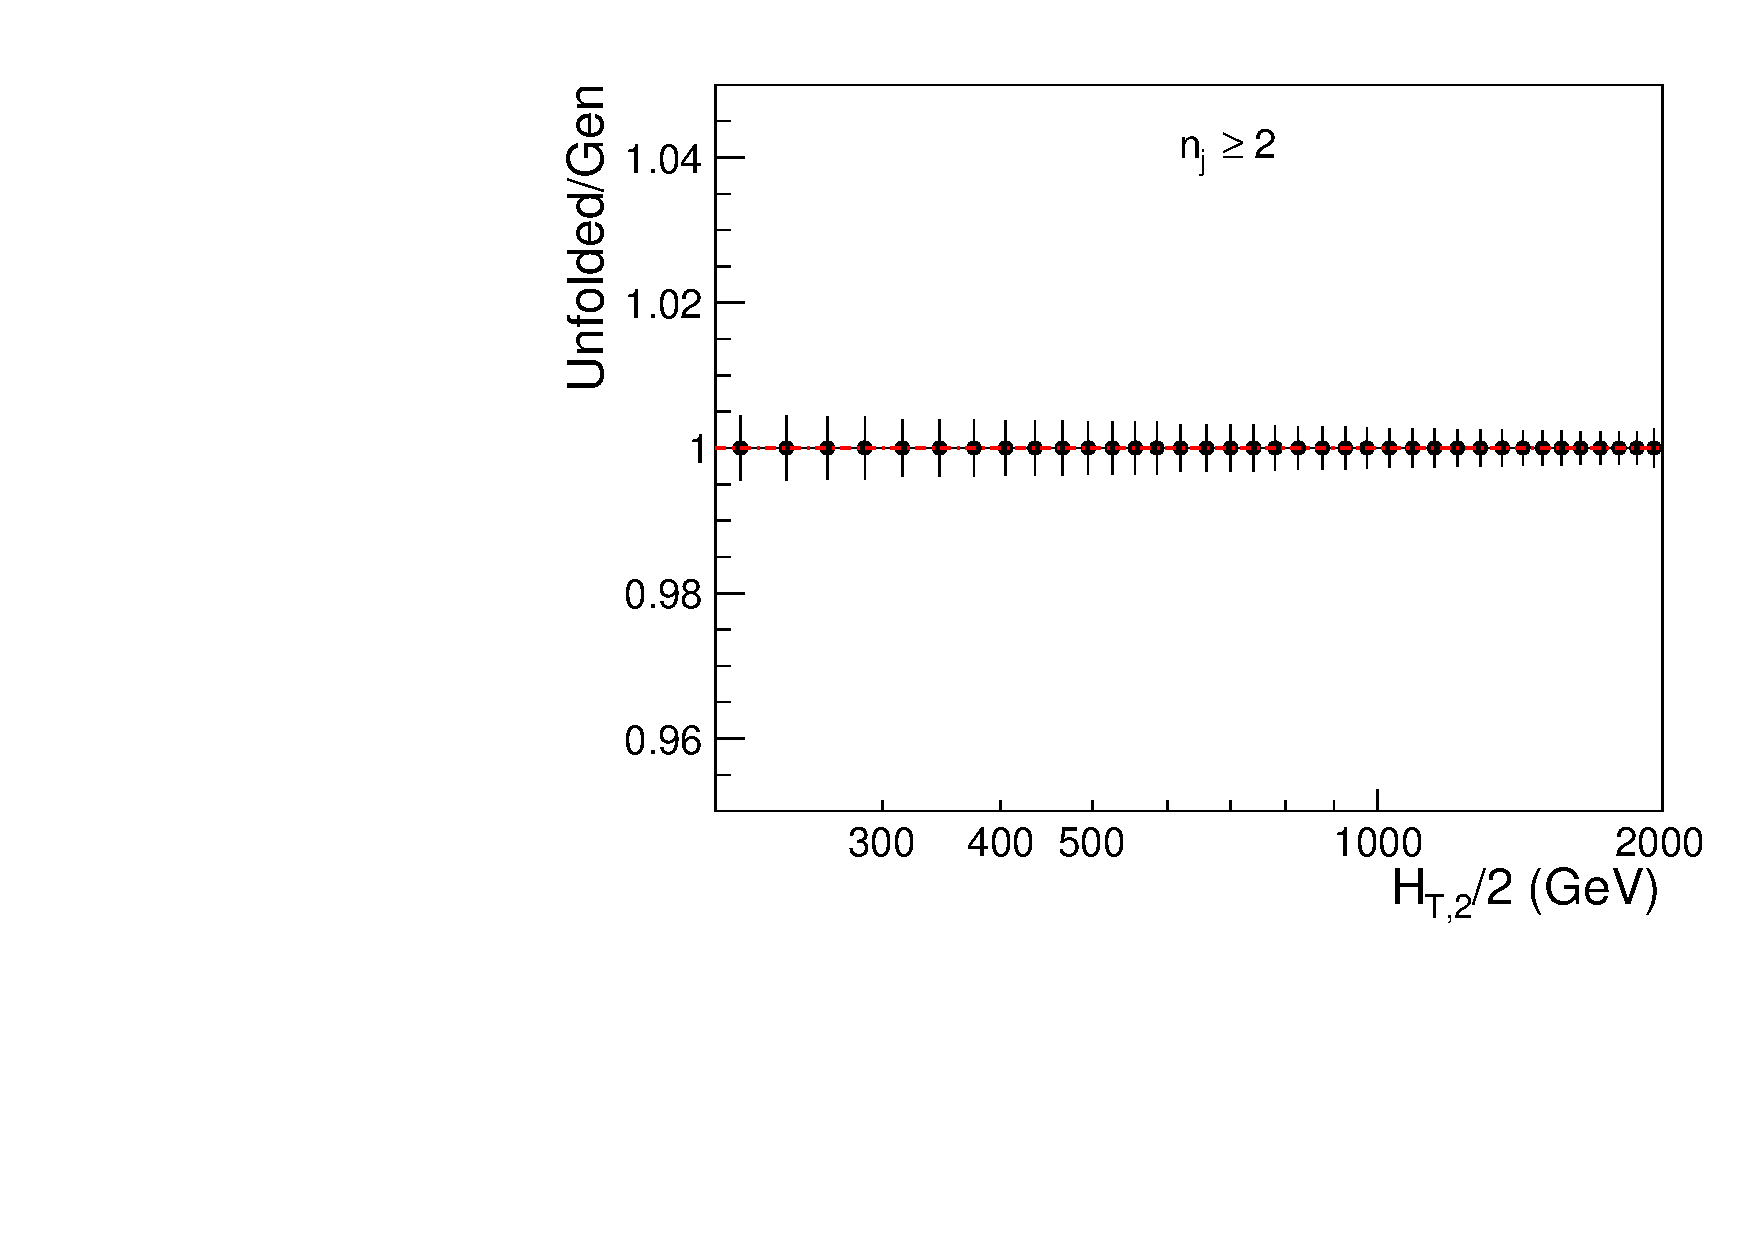
\includegraphics[width=0.5\textwidth]{Plots_HT_2_150/Ratio_Unfolding_NLO_2.pdf}%
    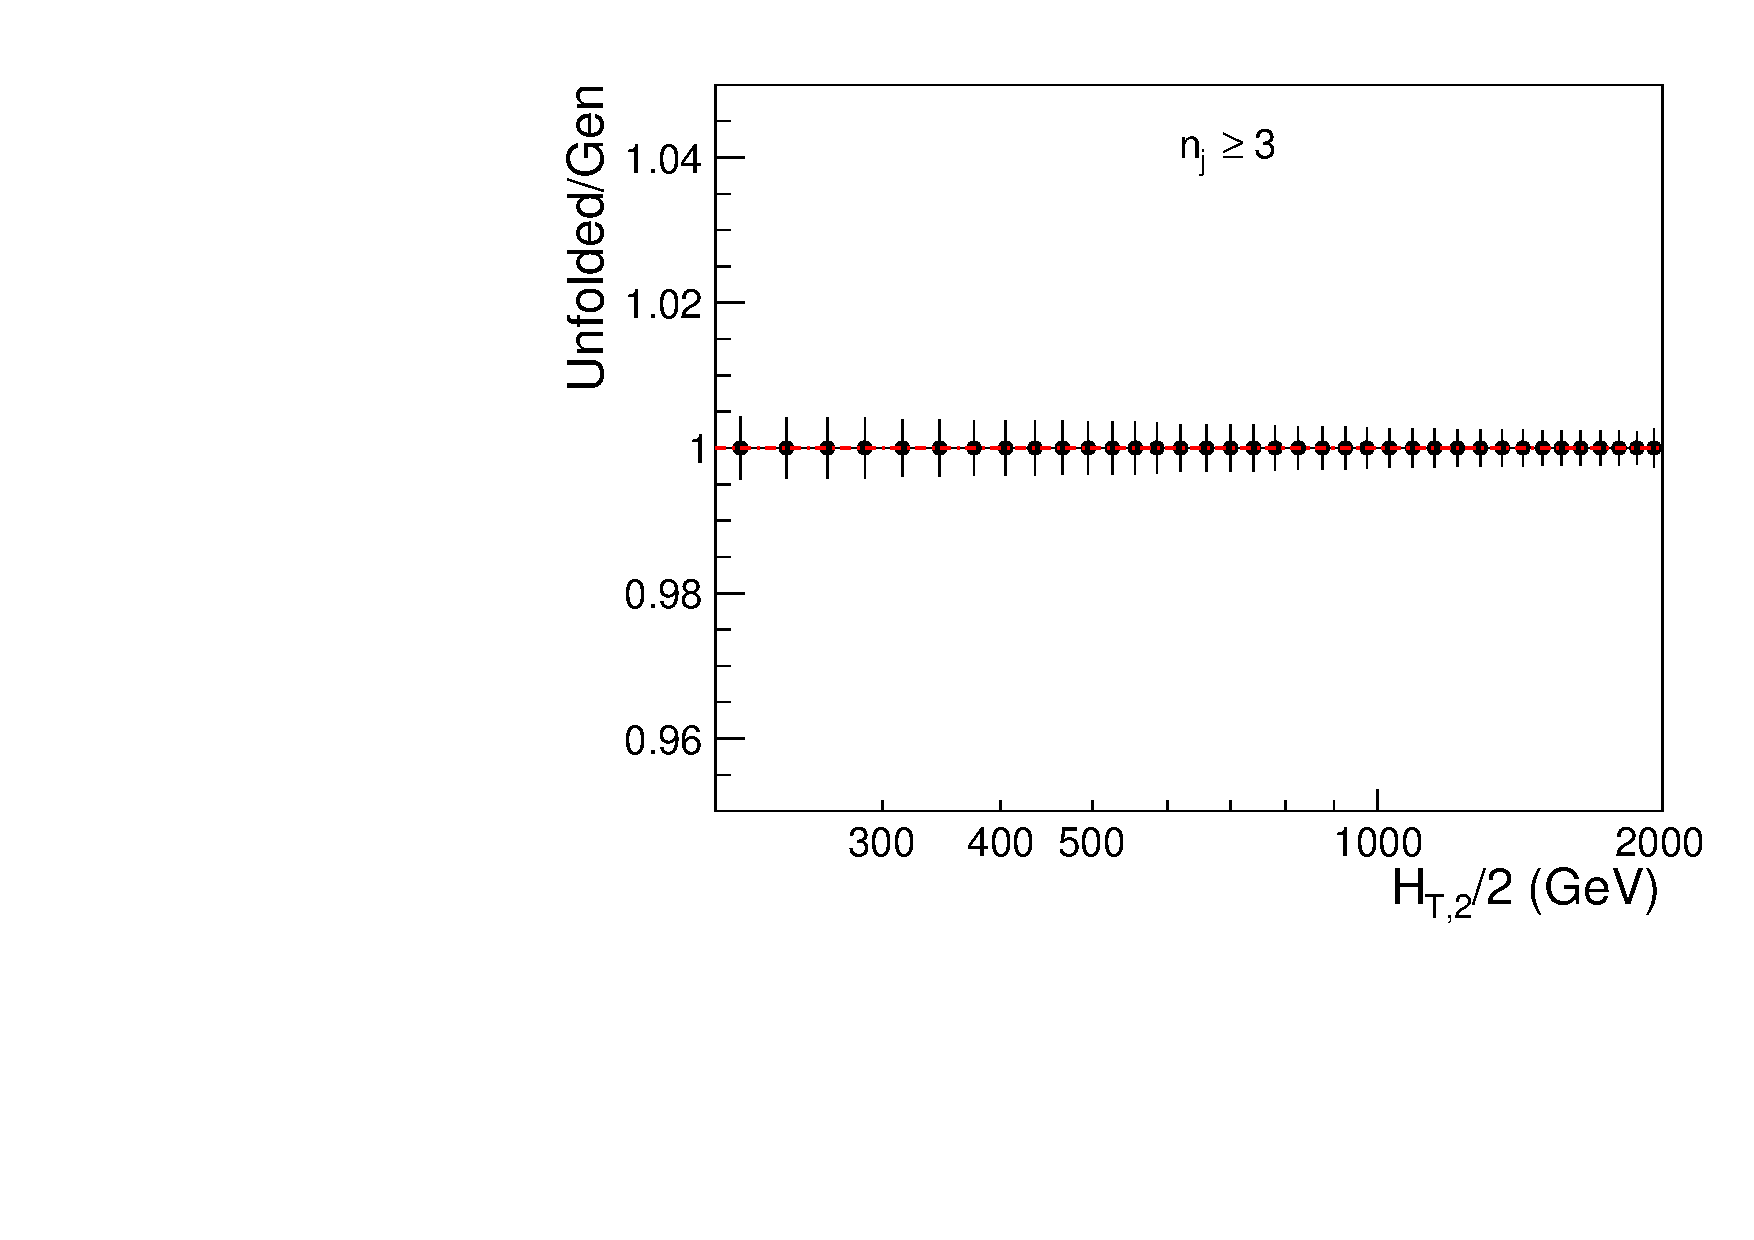
\includegraphics[width=0.5\textwidth]{Plots_HT_2_150/Ratio_Unfolding_NLO_3.pdf}
    \caption{Closure test with response matrices from NLO for inclusive 2-jet (left) and inclusive 3-jet events (right).}
    \label{fig:unfolded_smeared}
 
    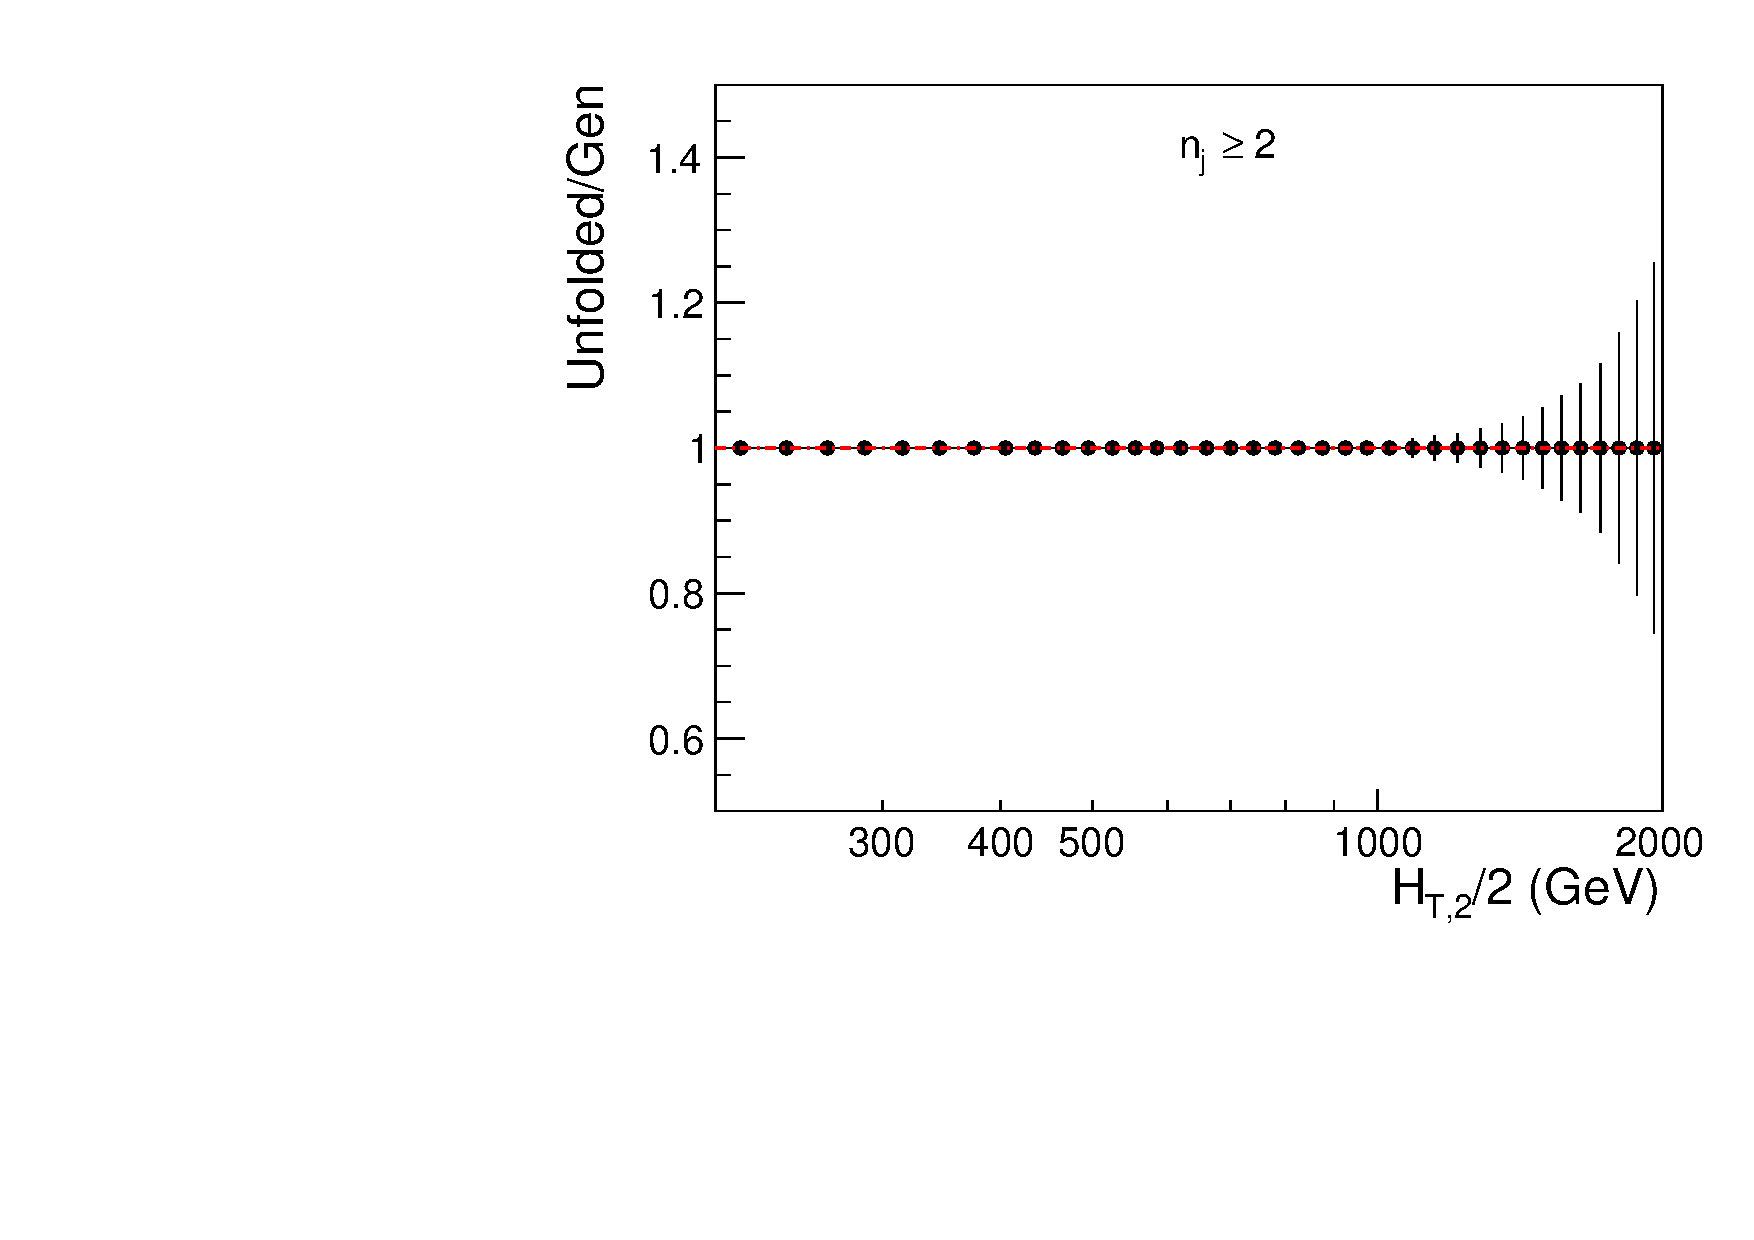
\includegraphics[width=0.5\textwidth]{Plots_HT_2_150/Ratio_Unfolding_Mad_2_HT_2_150.pdf}%
    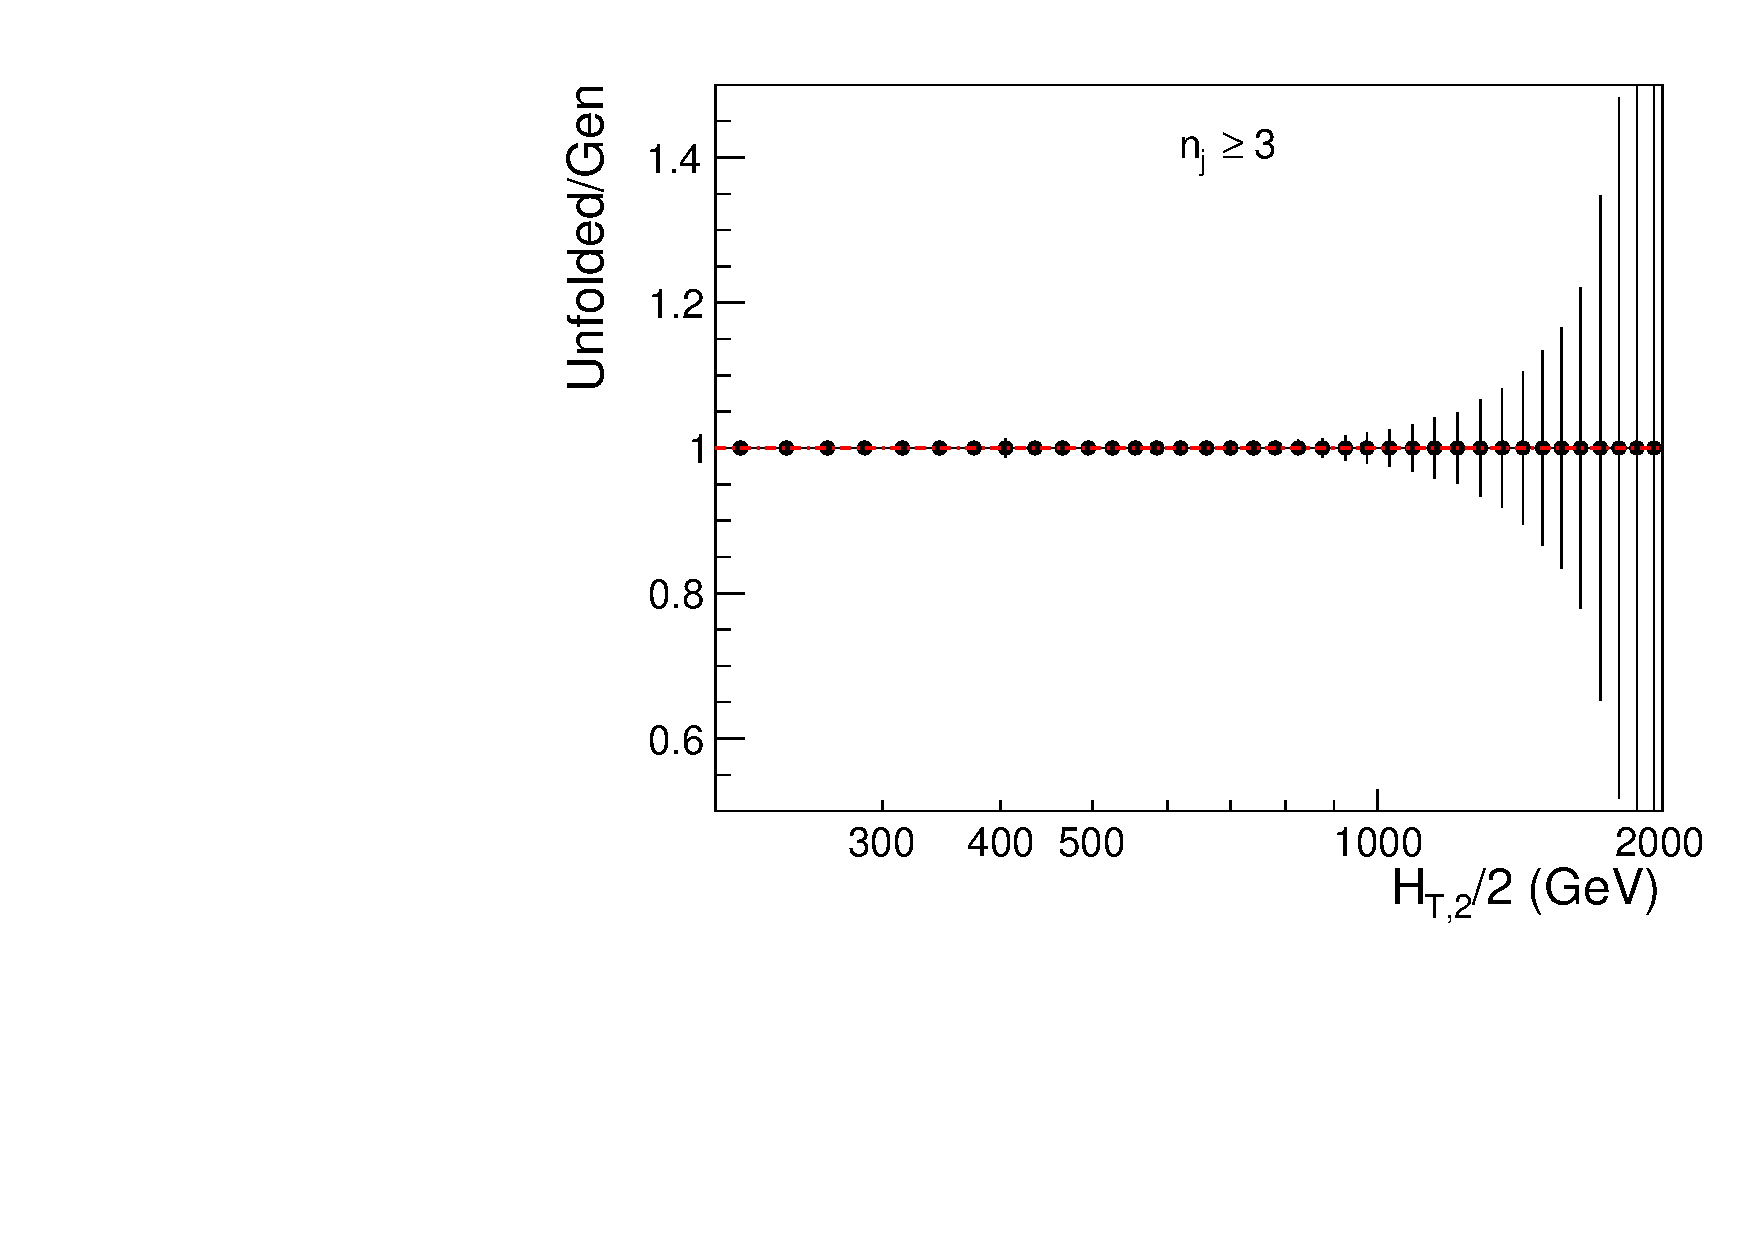
\includegraphics[width=0.5\textwidth]{Plots_HT_2_150/Ratio_Unfolding_Mad_3_HT_2_150.pdf}\\
    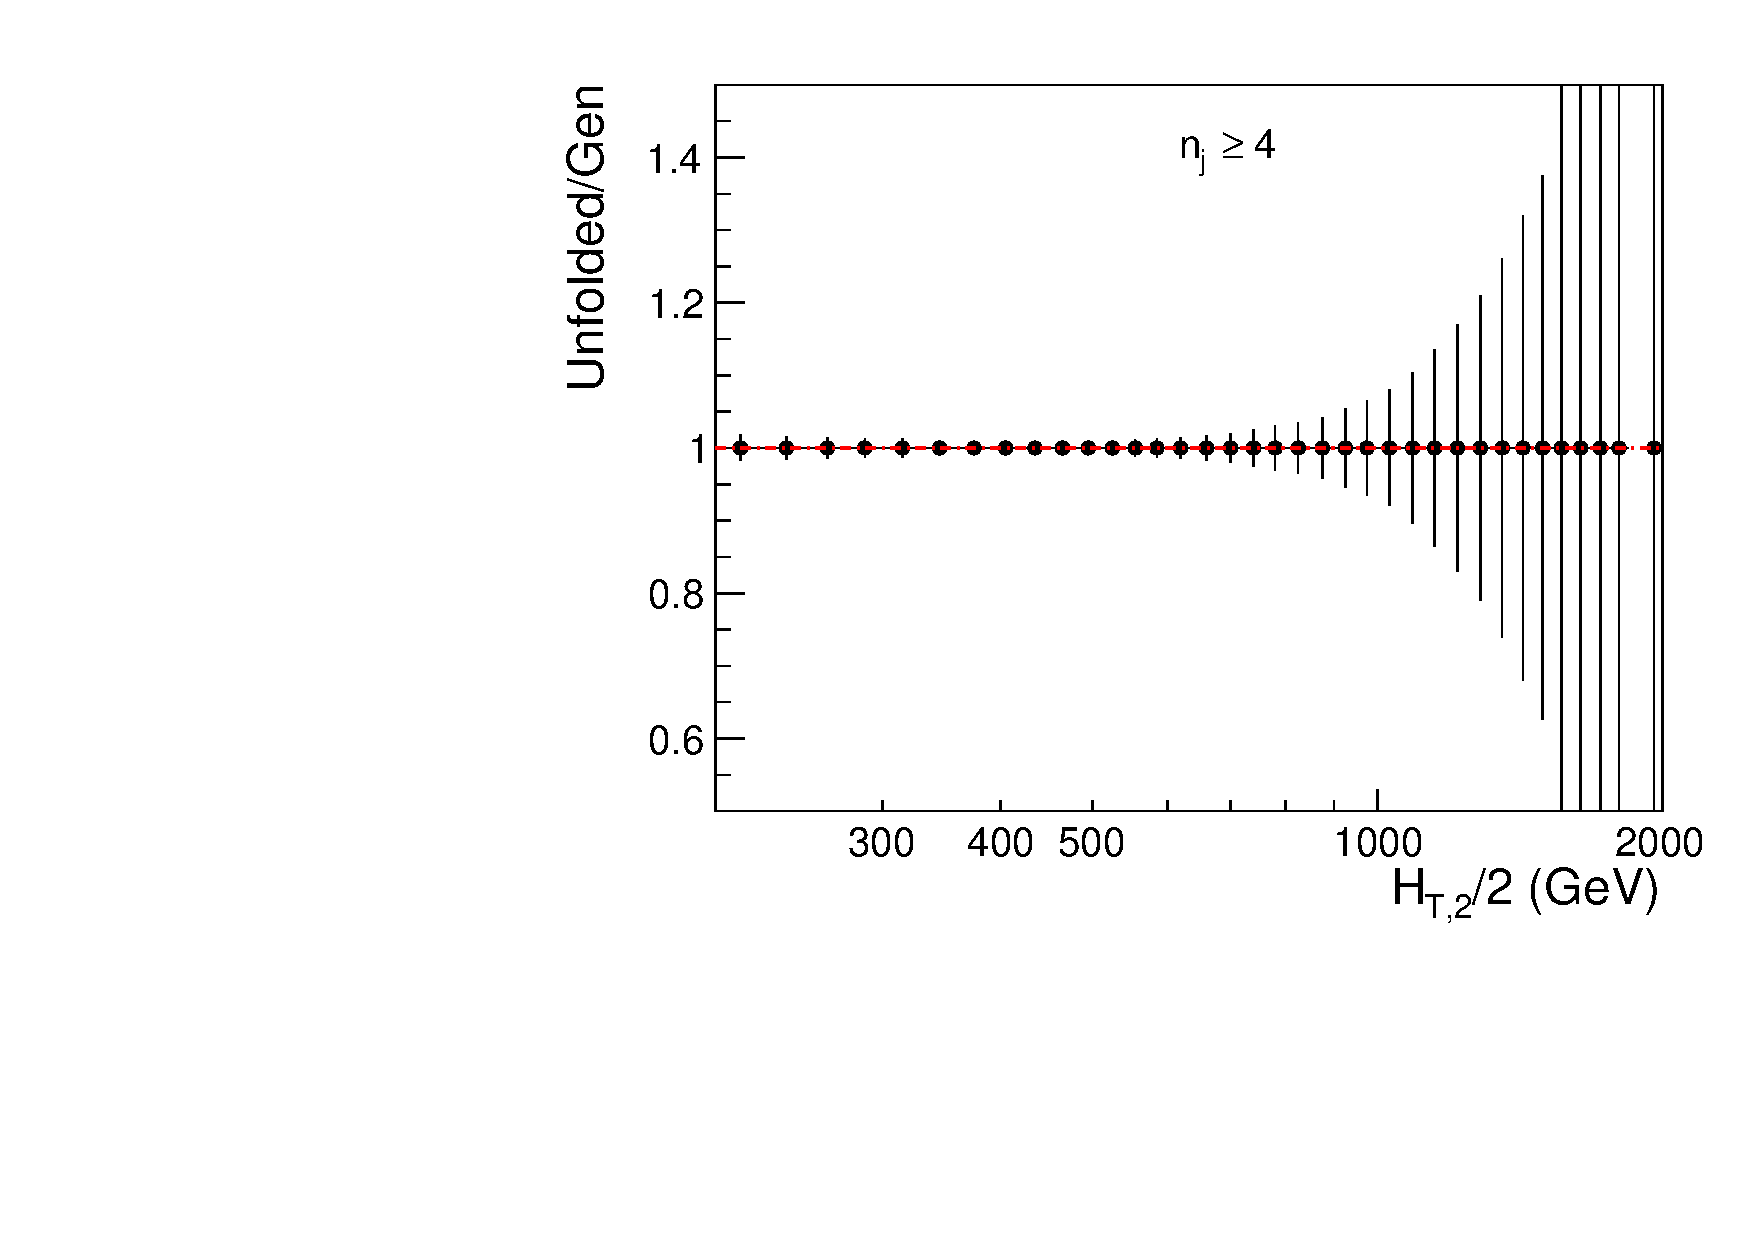
\includegraphics[width=0.5\textwidth]{Plots_HT_2_150/Ratio_Unfolding_Mad_4_HT_2_150.pdf}
    \caption{Closure test with response matrices from \MadGraphF + \PYTHIAS MC for inclusive 2-jet (top left), inclusive 3-jet events (top right) and inclusive 4-jet events (bottom).}
    \label{fig:unfolded_reco}
  \end{center}
\end{figure}

\begin{figure}[!htp]
  \begin{center}
    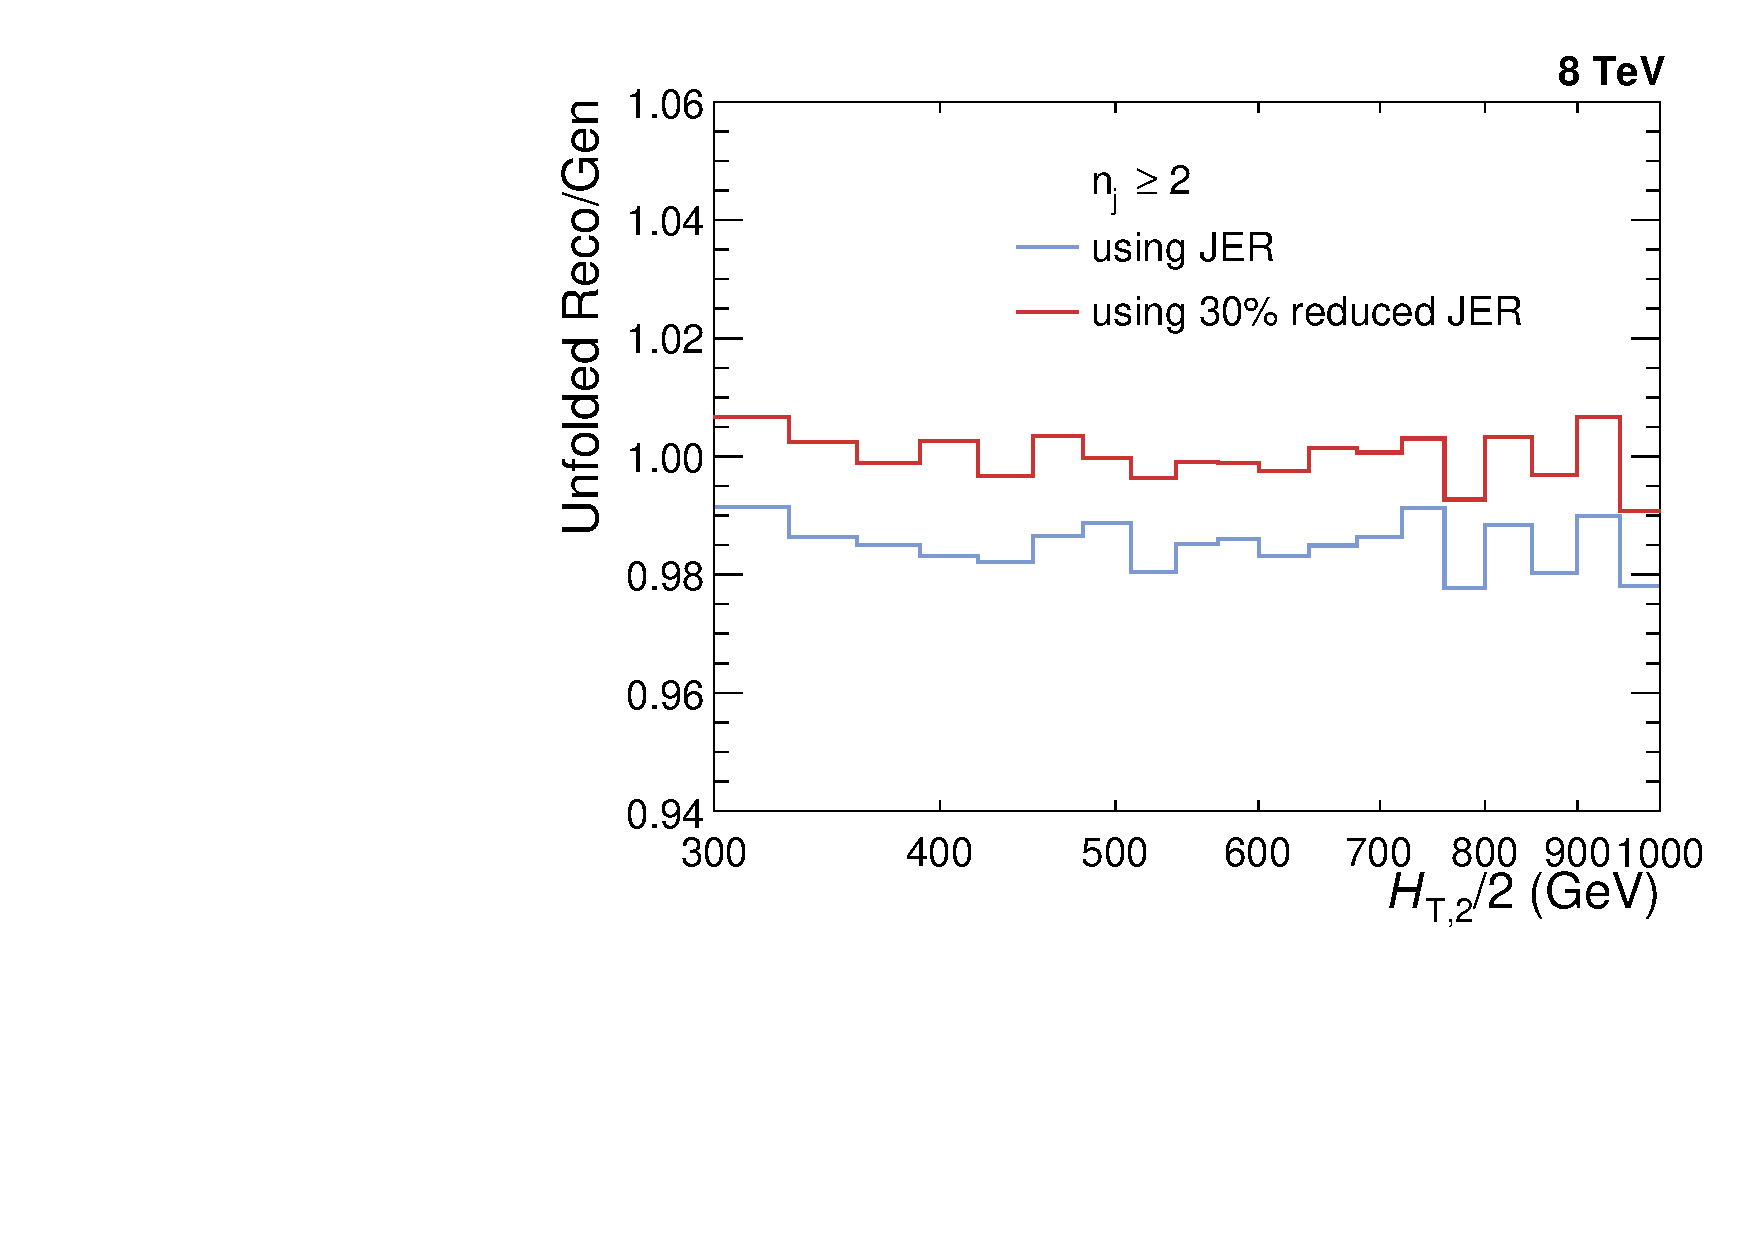
\includegraphics[width=0.5\textwidth]{Plots_HT_2_150/Comparison_closure_2_range.pdf}%
    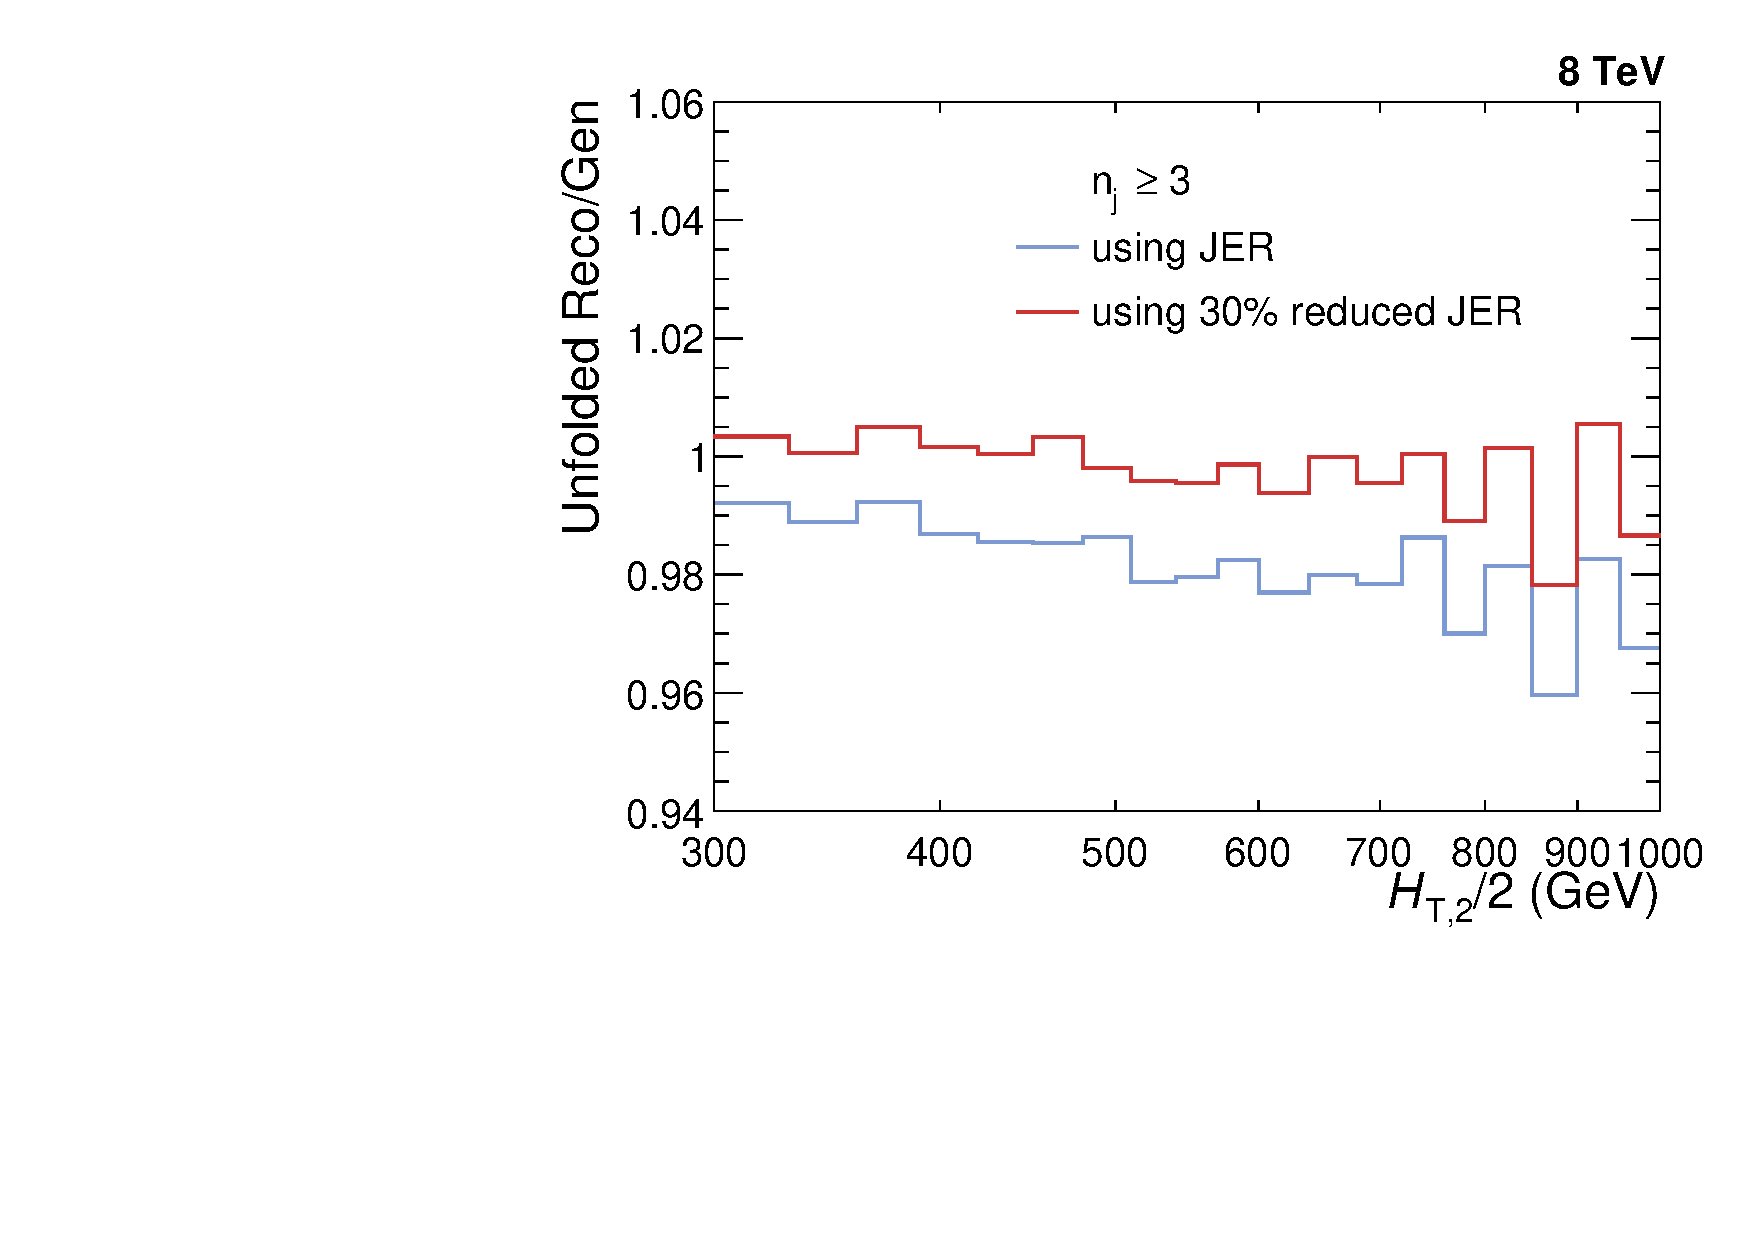
\includegraphics[width=0.5\textwidth]{Plots_HT_2_150/Comparison_closure_3.pdf}
    \caption{Closure test with unfolding \MadGraphF + \PYTHIAS Reco MC with response matrices from NLO for inclusive 2-jet (left) and inclusive 3-jet events (right).}
    \label{fig:unfolded_reco_NLO}

    \includegraphics[width=0.5\textwidth]{Plots_HT_2_150/Ratio_Unfolding_data_NLO_2.pdf}%
    \includegraphics[width=0.5\textwidth]{Plots_HT_2_150/Ratio_Unfolding_data_NLO_3.pdf}
    \caption{The ratio of data unfolded with that of measured using response matrices from NLO (black solid circles), from NLO but 30\% reduced JER (green solid circles) and from MC (red open circles); for inclusive 2-jet (left) and inclusive 3-jet events (right).}
    \label{fig:unfolded_data}
  \end{center}
\end{figure}

\subsubsection{Unfolding data}
After the validity of the unfolding method, the data is unfolded using the above reconstructed response matrices : both from NLO as well as 
MC. The unfolded data is compared to that of measured. Figure~\ref{fig:unfolded_data} shows the ratio of data unfolded to the measured data using response matrices from NLO (black solid circles), from NLO but 30\% reduced JER (green solid circles) and from MC (red open circles); for inclusive 2-jet (left) and inclusive 3-jet events (right). The unfolding using MC and reduced JER NLO response matrices, give similar results within statistical uncertainties. 
The unfolding does not 
working well for bins near to minimum \pt cut for inclusive 2-jet events because two-jet rate is very sensitive to soft gluon emission 
while the higher jet multiplicities are less affected. The event yield for each bin in \httwo is tabulated in Appendix in Table~\ref
{table_event}. 

\subsection{Experimental uncertainties}
\label{sec:exp_unc}
The experimental sources of uncertainty which affect the cross section measurement includes - 

\begin{itemize}
\item the statistical uncertainty : propagated through the unfolding, 
\item the jet energy corrections uncertainty (JEC) : uncertainty due to the calibration of the jet energy, 
\item the unfolding uncertainty : attributed by unfolding procedure,  
\item the luminosity uncertainty : arising from the imperfection of the CMS luminosity, 
\item an uncorrelated residual uncertainty of 1\% : which comprises the trigger efficiency uncertainty, the jet id efficiency and further residual effects.
\end{itemize}

\subsubsection{Uncertainty on luminosity measurement}
The uncertainty on the luminosity measurement for the 2012 LHC run is estimated to be 2.5\% (syst.) and 0.5\% (stat.)~\cite{CMS:2013gfa}. 
As the luminosity uncertainty translates into a normalization uncertainty on any absolute cross section measurement, a combined systematic 
uncertainty of 2.6\% is assigned which is fully correlated across all the \httwo bins. 

\subsubsection{Statistical uncertainty}
\label{sec:unfolding_stat}
Statistical uncertainties of data points are propagated through the unfolding using a toy MC technique in which the measured data points 
are smeared within their statistical uncertainties and the unfolding procedure is repeated multiple times for each smeared
spectra. One million of such toy spectra are used to propagate the statistical uncertainty. Figure~\ref{fig:stat_unc} shows the relative 
statistical uncertainty before and after the unfolding procedure. 

\begin{figure}[!htbp]
  \begin{center}
    \includegraphics[width=0.5\textwidth]{Plots_HT_2_150/Comparison_stat_unc_2_HT_2_150.pdf}%
    \includegraphics[width=0.5\textwidth]{Plots_HT_2_150/Comparison_stat_unc_3_HT_2_150.pdf}
    \caption{The fractional statistical uncertainties of the measured and the unfolded data for inclusive 2-jet events (left) and for 
      inclusive 3-jet events (right). Depending on the unfolding procedure, the uncertainties can slightly increase, which is observed.}
    \label{fig:stat_unc}
  \end{center}
\end{figure}

The uncertainty slightly increases during the unfolding process. Furthermore, the unfolding introduces a correlation between bins due to
event migrations. These correlations are significant for neighbouring bins in \httwo and negligible between bins far off in the phase 
space. Figure~\ref{fig:corr} shows the correlations of the statistical uncertainty after the unfolding. We studied the correlations by 
performing unfolding with taking 4, 5 and 10 iterations and choosing the unfolding iteration parameter as ``4'' ensures that the 
statistical errors in the unfolded distributions are greater than that of the measured distributions. 

\begin{figure}[!htbp]
  \begin{center}
    \includegraphics[width=0.35\textwidth]{Plots_HT_2_150/Correlation_Matrix_NLO_2_ite4.pdf}%
    \includegraphics[width=0.35\textwidth]{Plots_HT_2_150/Correlation_Matrix_NLO_2_ite5.pdf}%
    \includegraphics[width=0.35\textwidth]{Plots_HT_2_150/Correlation_Matrix_NLO_2_ite10.pdf}\\
    \vspace{5mm}
    \includegraphics[width=0.35\textwidth]{Plots_HT_2_150/Correlation_Matrix_NLO_3_ite4.pdf}%
    \includegraphics[width=0.35\textwidth]{Plots_HT_2_150/Correlation_Matrix_NLO_3_ite5.pdf}%
    \includegraphics[width=0.35\textwidth]{Plots_HT_2_150/Correlation_Matrix_NLO_3_ite10.pdf}%
    \caption{Correlations of the statistical uncertainty introduced by the unfolding procedure for inclusive 2-jet events (Top) and for 
      inclusive 3-jet events (Bottom) with 4 iterations (left), 5 iterations (middle) and 10 iterations (right). Neighbouring bins have a 
      significant correlation or anti-correlation through bin migrations.}
    \label{fig:corr}
  \end{center}
\end{figure}

\subsubsection{Jet Energy Scale uncertainty}
The systematic uncertainty on the measured cross sections is asymmetric and dominated by the uncertainty on the jet-energy corrections (JEC). This is estimated by shifting the jet \pt according to the JEC uncertainty. The JEC uncertainties are split 
into 25 mutually independent sources of uncertainty, in which each source is fully correlated in \pt and $\eta$ but uncorrelated to all 
other sources and presents a 1$\sigma$ shift. \httwo is calculated by varying \pt and the difference from central \httwo gives JEC uncertainty as a function of \httwo. As these uncertainties can be asymmetric, the upwards and downwards variation of each source 
are treated separately. The sum in quadrature of all sources yields the total JEC uncertainty.

The sources of uncertainty are grouped in four categories according to their origin and details about the jet energy corrections and 
uncertainties are given in~\cite{bib:JES_2013} and in : \\
https://twiki.cern.ch/twiki/bin/viewauth/CMS/ JECUncertaintySources\#Winter14\_uncertainties. 

The 25 individual uncertainty sources are the following :
AbsoluteStat, AbsoluteScale, AbsoluteFlavMap, AbsoluteMPFBias, Fragmentation, SinglePionECAL, 
SinglePionHCAL, FlavorQCD, RelativeJEREC1, RelativeJEREC2, RelativeJERHF,
RelativePtBB, RelativePtEC1, RelativePtEC2, RelativePtHF, RelativeFSR, RelativeStatFSR, RelativeStatEC2,
RelativeStatHF, PileUpDataMC, PileUpPtRef, PileUpPtBB, PileUpPtEC1, PileUpPtEC2 and PileUpPtHF.

The AbsoluteFlavMap uncertainty is exactly zero for the 8 TeV and can be ignored. In this way practically 24 uncertainties are considered to calculate JEC uncertainty. For the four sources : RelativeJERHF, 
RelativePtHF, RelativeStatHF, PileUpPtHF, the JEC uncertainty is exactly zero because of \abs{y} $<$ 2.5 cut used in the analysis. So only 20 sources contribute to the total JEC uncertainty. The Figures~\ref{fig:jes1}-\ref{fig:jes4} show the JEC uncertainty from each 
source separately for inclusive 2-jet (left) and 3-jet events (middle), respectively. The bin-wise values (in \%) are tabulated in the Tables~\ref{tab:exp_unc_jes_2},~\ref{tab:exp_unc_jes_2s} for inclusive 2-jet and~\ref{tab:exp_unc_jes_3},~\ref{tab:exp_unc_jes_3s} for inclusive 3-jet events. 

\subsubsection{Unfolding uncertainty}
\label{sec:unfolding_unc}
The unfolding uncertainty is comprised of three uncertainties :

\begin{enumerate}
\item {\bf JER uncertainty :} The jet energy resolution, which was derived in Section~\ref{subsec:Resolution}, is used to produce the response matrix using a forward 
smearing technique in the unfolding procedure. Therefore, a dependence on the jet energy resolution on the unfolded cross section is 
introduced and a further uncertainty source due to the uncertainty on the jet energy resolution is introduced. Table~\ref{resolution} shows 
the scaling factors, which were applied on reconstructed simulated events to obtain the actual resolution in data. The official 
recommendations include offset variations of these scaling factors to estimate the uncertainty on the resolution and are also given in Table~\ref{resolution}. The 
determination of the resolution is repeated with the upwards and downwards variation of the resolution scaling factor applied. The 
unfolding procedure is also reiterated using the variations of the resolution and the differences of the obtained cross section to the 
nominal cross section are accounted for as a systematic uncertainty. 

\item {\bf Model dependence :} As explained earlier that to construct the response matrix by Toy MC method, the fitting of the theoretical predictions is performed by using function given in Equation~\ref{eq:func1}. To use alternative function for this fitting gives the model dependence of the theoretical \httwo spectrum which affects the response matrix and thus the unfolding.
The NLO \httwo spectrum is fitted by the another function described by Equation~\ref{eq:func2}. The procedure mentioned in Section~\ref
{sec:unfolding} is repeated to get the new unfolded cross sections. The differences in unfolded cross sections using the functions given by equations~
\ref{eq:func1} and~\ref{eq:func2} gives the unfolding uncertainty. 

\item {\bf Additional uncertainty :} As explained in Section~\ref{subsec:Resolution}, an additional uncertainty is added from the difference in unfolding on comparing with reduced JER.

\end{enumerate}

All the three uncertainties are added in quadrature to account the unfolding uncertainty which is 1-2\% on cross-sections.

\subsubsection{Total experimental uncertainty}
After calculating the uncertainties from all different sources, total experimental uncertainty is obtained by adding in quadrature the 
uncertainties from individual sources. The bin-wise values (in \%) of uncertainties from each source as well as total uncertainty are tabulated in Table~\ref{tab:exp_unc2} and Table~\ref{tab:exp_unc3} for inclusive 2-jet and inclusive 3-jet events, respectively. Figure~\ref{fig:exp_unc} show the uncertainties from all sources of 
experimental uncertainty as well as the total uncertainty for inclusive 2-jet (left) and inclusive 3-jet (right) events. The systematic uncertainty on the measured cross 
sections is asymmetric and dominated by the uncertainty on the jet-energy scale at lower \httwo values and by statistical uncertainty at 
higher \httwo values. The experimental uncertainties from each source as well as total uncertainty are quoted in Table~\ref{tab:exp_unc_overview}. 

\begin{figure}[!htbp]
  \begin{center}
    \includegraphics[width=0.5\textwidth]{Plots_HT_2_150/Total_unc_all_2_NLO_add.pdf}%
    \includegraphics[width=0.5\textwidth]{Plots_HT_2_150/Total_unc_all_3_NLO_add.pdf}
    \caption{Overview of all experimental uncertainties affecting the cross section measurement for inclusive 2-jet (left) and inclusive 3-
      jet (right). The error bars indicate the statistical uncertainty after unfolding. The colored lines give the uncertainties resulting of 
      jet energy scale, luminosity, unfolding and residual effects. The total uncertainty is calculated by adding in 
      quadrature the individual sources of uncertainty.}
    \label{fig:exp_unc}
  \end{center}
\end{figure}

\begin{table}[!htbp]
\caption{Overview of all experimental uncertainties affecting the cross section measurement.}
\label{tab:exp_unc_overview}
  \centering
  \begin{tabular}{ccc}
    \hline\hline
     Uncertainty Source & {\bf Inclusive 2-jet} & {\bf Inclusive 3-jet} \rbthm\\\hline     
     {\bf Statistical}  & $<$ 1 to 30\% & $<$ 1 to 40\% \rbtrr\\
     {\bf \blue {JEC}}  & 3 to 10\% & 4 to 12\% \rbtrr\\
     {\bf \textcolor{green!50!black} {Unfolding}} & 1-2\% & 1-2\% \rbtrr\\
     {\bf \mycolor {Luminosity}} & 2.6\% & 2.6\% \rbtrr\\
     {\bf \textcolor{red!30!blue!50!white} {Residual uncorrelated}} & 1\% & 1\% \rbtrr\\
  \hline\hline
  \end{tabular}
\end{table}

\section{Measurement of cross section ratio, unfolding and experimental uncertainties}
\subsection{Measurement of cross section ratio}
The ratio of cross sections, $R_{mn}$ as a function of $\httwo$, is extracted by dividing the cross section of selected inclusive m-jet 
events to that of inclusive n-jet events at any given bin size of \httwo. The ratios \ratio, $R_{43}$ and $R_{42}$ are calculated. In cross 
section ratios, the numerator and denominator are not independent samples. So to calculate the statistical uncertainty for the cross 
section ratios before unfolding, the Wilson score interval is used which takes into account the correlation between the numerator and the denominator and 
give asymmetric errors. For example, the bin-wise inclusive 2-jet and 3-jet differential cross sections as well as cross section ratio \ratio, calculated at detector level, along with statistical uncertainty (in \%) are tabulated in Table~\ref{tab:ratio_32}. 

Figure~\ref {fig:ratio_32} shows the ratio $R_{mn}$ as a function of $\httwo$ : \ratio data (black solid circles), \ratio~\MadGraphF + \PYTHIAS MC 
(red solid circles) and \ratio NLO (green solid line), $R_{43}$ data (black solid triangles (up)), $R_{43}$ \MadGraphF + \PYTHIAS MC (red 
solid triangles (up)) and $R_{42}$ data (black solid triangles (down)), $R_{42}$ \MadGraphF + \PYTHIAS MC (red solid triangles (down)). The 
ratios $R_{mn}$ from data are in well agreement with that from MC as well as NLO predictions.

\begin{figure}[!htbp]
  \begin{center}
    \includegraphics[width=0.5\textwidth]{Plots_HT_2_150/Ratio_32_43_42_all_HT_2_150.pdf}
    \caption{Cross section ratios $R_{mn}$ as a function of $\httwo$. The error bars give the statistical uncertainty, calculated by the Wilson score interval which takes into the account the correlation between the numerator and the denominator.}
    \label{fig:ratio_32}
  \end{center}
\end{figure}

\subsection{Unfolding}
The measured ratio \ratio as a function of \httwo, is then corrected for detector smearing effects and unfolded to particle level. There can be two ways to obtain  unfolded cross section ratio :

\begin{enumerate}
\item To unfold separately the inclusive 2-jet and 3-jet measured cross sections and then construct the ratio \ratio 
\item To unfold directly the ratio \ratio
\end{enumerate}

%Both methods gave the same results. 
In the first method, we have ratios of unfolded cross sections by using response matrices constructed using Toy MC method i.e. smeared NLO matrices (Figure~\ref{fig:response_NLO}) as well as by using response matrices from \MadGraphF + \PYTHIAS MC (Figure~\ref{fig:response_MC}). Figure~\ref{fig:ratio_unfolded_32} left shows the comparison of \ratio, obtained from data unfolded using smeared NLO matrix (black solid circles) and the one unfolded using MC matrix (red solid circles), with \ratio from NLO prediction (red line). As the matrices from MC are also available for inclusive 4-jet events, so these can used to unfold the ratios $R_{43}$ and $R_{42}$ as shown in Figure~\ref{fig:ratio_unfolded_32} with black solid triangles (up) and black solid triangles (down), respectively.

In further analysis, cross section ratio obtained from data, unfolded using smeared NLO matrix is considered. Since the theory NLO predictions are available for inclusive 2-jet and 3-jet events and not for inclusive 4-jet events yet, so only ratio \ratio is used in further analysis. Figure~\ref{fig:ratio_unfolded_32} right gives the ratio of unfolded \ratio calculated from ratio of unfolded cross sections to that of measured one using central JER (black solid circles) as well as reduced JER (green solid circles).  We have used first method to calculate the systematic uncertainties.

 \begin{figure}[!htbp]
  \begin{center}
    \includegraphics[width=0.5\textwidth]{Plots_HT_2_150/Ratio_32_43_42_unfolded_all_HT_2_150.pdf}%
    \includegraphics[width=0.5\textwidth]{Plots_HT_2_150/Ratio_Unfolding_data_NLO_ratio32.pdf}\\
    \caption{Left figure shows the unfolded \ratio,  obtained from data unfolded using smeared NLO matrix (black solid circles), from data unfolded using MC matrix (red 
    solid circles) and from NLO prediction (red line); $R_{43}$ from the data unfolded using MC matrix (black solid triangles (up)) and $R_
    {42}$ from data unfolded using MC matrix (black solid triangles (down)). Right gives the ratio of unfolded \ratio calculated from ratio of unfolded cross sections to that of measured one using central JER (black solid circles) as well as reduced JER (green solid circles).}
    \label{fig:ratio_unfolded_32}
  \end{center}
\end{figure}

\subsubsection{Response matrix}
To unfold directly the ratio \ratio, we need to construct the response matrix using Toy MC method as explained in section~\ref
{sec:unfolding}. To obtain the true spectrum for \ratio, the ratio of theory predictions, extrapolated with function I (equation~\ref
{eq:func1}, for inclusive 3-jet to that of 2-jet is taken, as shown in Figure~\ref{fig:fit} (Top). Then this ratio is fitted using the polynomial function of degree 8 as shown in Figure~\ref{fig:ratio_fit}.
 
 \begin{figure}[!htbp]
  \begin{center}
    \includegraphics[width=0.6\textwidth]{Plots_HT_2_150/Extrapolate_Theory_Ratio_32.pdf}
    \caption{Fitted NLO spectrum of cross section ratio \ratio as a function of \httwo using polynomial function of degree 8.}
    \label{fig:ratio_fit}
  \end{center}
\end{figure}

A flat \httwo spectrum is generated and the fit parameters obtained from polynomial fit provides weights to the flat spectrum. A total of 
ten million events are generated (in \httwo range 80-2000). These generated values are smeared with a Gaussian function, where $\sigma$ of 
the Gaussian is determined from the relative resolution parametrization as a function of \httwo calculated from NSC formula mentioned in 
equation~\ref{NSC_formula}. The parameters N, S, C used for smearing are taken to be same for inclusive 3-jet events, as mentioned in Table~\ref{fit_para}.

These generated and smeared values are used to fill the response matrices by using the RooUnfold package. Figure~\ref
{fig:unfolded_ratio} (left) shows the response matrix derived using the Toy MC for ratio \ratio. The matrix is normalized to the number of 
events in each column. The response matrix is diagonal with small off-diagonal migrations between close-by \httwo bins.

First we unfold the smeared spectrum obtained from Toy MC to perform the closure test. Figure~\ref{fig:unfolded_ratio} (right) shows 
that after unfolding, the smeared spectrum matches exactly with the randomly generated spectrum as expected. The bottom plot gives the ratio of unfolded 
%ratio calculated from the unfolded cross sections to that of the measured one. The unfolding works well above 300 GeV and considering the the lack of statistical precision beyond 1680 GeV for inclusive 3-jet events (from Table~\ref{tab:ratio_32}), the ratio distributions are plotted in the range 300-1680 GeV. 
%Then the measured ratio \ratio 
%from data is unfolded using the above reconstructed response matrix. The unfolded \ratio is compared to that of measured (bottom left) 
%in Figure~\ref{fig:unfolded_ratio}. As explained earlier, the Wilson score interval method to calculate the statistical uncertainty on the 
%measured ratio, gives the asymmetric statistical errors. So the measured ratio is unfolded two times : once with Up and and then with Low 
%statistical errors to get the asymmetric statistical uncertainties after unfolding. The right hand side plot gives the ratio of unfolded 
%ratio calculated from the unfolded cross sections to that of the measured one. The unfolding works well above 300 GeV and considering the the lack of statistical precision beyond 1680 GeV for inclusive 3-jet events (from Table~\ref{tab:ratio_32}), the ratio distributions are plotted in the range 300-1680 GeV.
\begin{figure}[!htbp]
  \begin{center}
    \includegraphics[width=0.45\textwidth]{Plots_HT_2_150/Normalized_Response_Matrix_NLO_ratio_32_column_2.pdf}
    \includegraphics[width=0.45\textwidth]{Plots_HT_2_150/Ratio_Unfolding_NLO_Ratio_32_ToyMC.pdf}\\
    %\includegraphics[width=0.45\textwidth]{Plots_HT_2_150/Ratio_Unfold_data_ratio_32_direct_ToyMC.pdf}
    %\includegraphics[width=0.45\textwidth]{Plots_HT_2_150/Ratio_Unfold_data_ratio_32_unfoldedx.pdf}
    \caption{The response matrix derived using the Toy MC for ratio \ratio (left) and Closure test (right).}% and ratio of unfolded direct \ratio to that of measured (bottom left), with statistical uncertainties Up (solid line) as well as statistical uncertainties Low (dashed line),     The ratio of unfolded \ratio calculated from ratio of unfolded cross sections to that of measured one (bottom).}
    \label{fig:unfolded_ratio}
  \end{center}
\end{figure}

\subsection{Experimental uncertainties}
In cross section ratio, the uncorrelated and luminosity uncertainties got cancel. The experimental sources of uncertainty which affect the cross section ratio measurement includes - 

\begin{itemize}
\item the statistical uncertainty : propagated through the unfolding, 
\item the jet energy correction uncertainty (JEC) : uncertainty due to the calibration of the jet energy, 
\item the unfolding uncertainty : unfolding procedure.
\end{itemize}

\subsubsection{Statistical uncertainty}
\label{sec:unfolding_stat_ratio}
The statistical uncertainties for ratio \ratio are calculated in the same way as it was done for inclusive 2-jet and 3-jet cross sections, explained in section~\ref{sec:unfolding_stat}. Figure~\ref{fig:stat_unc_ratio} shows the relative statistical uncertainty before and after the unfolding procedure. 

\begin{figure}[!htbp]
  \begin{center}
    \includegraphics[width=0.5\textwidth]{Plots_HT_2_150/Comparison_stat_unc_ratio_32_up.pdf}%
    \includegraphics[width=0.5\textwidth]{Plots_HT_2_150/Comparison_stat_unc_ratio_32_down.pdf}\\
    \caption{The fractional statistical uncertainties Up (left) and Low (right), of the unfolded as well as measured cross section ratio \ratio. Depending on the unfolding procedure, the uncertainties can slightly increase, which is observed.}
    \label{fig:stat_unc_ratio}
  \end{center}
\end{figure}

The uncertainty slightly increases during the unfolding process. Also, the unfolding introduces a correlation between bins due to
event migrations. To find the correlations of the statistical uncertainty introduced by the unfolding procedure for ratio, \ratio, firstly 
ratio is calculated and then unfolded this ratio to particle level. Figure~\ref{fig:corr_ratio} shows the correlations of the statistical 
uncertainty after the unfolding. We studied the correlations by performing unfolding with taking 4, 5 and 10 iterations and choosing the 
unfolding iteration parameter as ``4'' ensures that the statistical errors in the unfolded distributions are greater than that of the 
measured distributions. 

\begin{figure}[!htbp]
  \begin{center}
    \includegraphics[width=0.35\textwidth]{Plots_HT_2_150/Correlation_Matrix_NLO_Ratio_32_ite4.pdf}%
    \includegraphics[width=0.35\textwidth]{Plots_HT_2_150/Correlation_Matrix_NLO_Ratio_32_ite5.pdf}%
    \includegraphics[width=0.35\textwidth]{Plots_HT_2_150/Correlation_Matrix_NLO_Ratio_32_ite10.pdf}\\
    \caption{Correlations of the statistical uncertainty introduced by the unfolding procedure for ratio \ratio with 4 iterations (left), 5 iterations (middle) and 10 iterations (right). Neighbouring bins have a significant correlation or anti-correlation through bin migrations.}
    \label{fig:corr_ratio}
  \end{center}
\end{figure}

\subsubsection{Jet Energy Scale uncertainty}
The systematic uncertainty on the measured cross sections is asymmetric and dominated by the uncertainty on the jet-energy correction (JEC) at low \httwo. To calculate JEC uncertainty for ratio \ratio, the inclusive 2-jet and 3-jet events cross sections are measured as a function of \httwo by shifting the jet \pt according to the JEC uncertainty for each source separately. Then the ratio of these cross sections, \ratio is taken and the difference from the central ratio \ratio, gives the JEC uncertainty for each source. As these uncertainties can be asymmetric, the upwards and downwards variation of each source are treated separately. The sum in quadrature of all sources yields the total JEC uncertainty.

The Figures~\ref{fig:jes1}-\ref{fig:jes4} show the JEC uncertainty from each source separately for ratio \ratio (right). As expected, the JEC uncertainty for ratio is less than that for inclusive cross sections. The bin-wise values (in \%) are tabulated in the Tables~\ref{tab:exp_unc_jes_r} and ~\ref{tab:exp_unc_jes_rs}.

\subsubsection{Unfolding uncertainty}
\label{sec:unfolding_unc_ratio}
As explained earlier in section~\ref{sec:unfolding_unc}, the three uncertainties are considered for \ratio :

\begin{enumerate}
\item {\bf JER uncertainty :} To determine JER uncertainty, ratio \ratio is calculated from the cross sections as a function of \httwo measured with the upwards and downwards variation of the resolution scaling factor as described in section~\ref{sec:unfolding_unc}. The differences of the obtained cross section ratio to the nominal cross section ratio are accounted as a systematic uncertainty. 

\item {\bf Model dependence : } As explained earlier in section~\ref{sec:unfolding_unc}, the differences in cross section ratios obtained from unfolded cross sections using the functions given by equations~\ref{eq:func1} and~\ref{eq:func2} gives the unfolding uncertainty. 

\item {\bf Additional uncertainty : } The additional uncertainty resulting from differences in unfolded cross-sections with central JER and 30\% reduced JER is added.

\end{enumerate}

All the three uncertainties are added to the unfolding uncertainty which is 1\% for \ratio.

\subsubsection{Total experimental uncertainty}
After calculating the uncertainties from all different sources, total experimental uncertainty is obtained by adding in quadrature the 
uncertainties from individual sources. The bin-wise values (in \%) of uncertainties from each source as well as total uncertainty are tabulated in Table~\ref{tab:exp_unc_ratio}. Figure~\ref{fig:exp_unc_ratio} show the uncertainties from all sources of 
experimental uncertainty as well as the total uncertainty. The systematic uncertainty on the measured cross 
sections is asymmetric and dominated by the uncertainty on the jet-energy scale at lower \httwo values and by statistical uncertainty at 
higher \httwo values. The experimental uncertainties from each source as well as total uncertainty are quoted in Table~\ref{tab:exp_unc_overview}.

\begin{figure}[!htbp]
  \begin{center}
    \includegraphics[width=0.5\textwidth]{Plots_HT_2_150/Total_Unc_ratio_32_direct_add.pdf}
    \caption{Overview of all experimental uncertainties affecting the cross section \ratio as a function of \httwo. The error bars indicate the statistical uncertainty. The colored lines give the uncertainties resulting of jet energy scale and unfolding. The total uncertainty is calculated by adding in quadrature the individual sources of uncertainty.}
    \label{fig:exp_unc_ratio}
  \end{center}
\end{figure}

\begin{table}[!htbp]
\caption{Overview of all experimental uncertainties affecting the cross section ratio, \ratio.}
\label{tab:exp_unc_ratio_overview}
  \centering
  \begin{tabular}{cc}
    \hline\hline
     Uncertainty Source & {\bf Ratio \ratio}  \rbthm\\\hline
     {\bf Statistical}  & $<$ 1 to $>$ 50\%  \rbtrr\\
     {\bf \blue {JEC}}  & 1 to 2\% \rbtrr\\
     {\bf \textcolor{green!50!black} {Unfolding}} & 1\%  \rbtrr\\
     {\bf \mycolor {Luminosity}} & cancels \rbtrr\\
     {\bf \textcolor{red!30!blue!50!white} {Residual uncorrelated}} & cancels \rbtrr\\
  \hline\hline
  \end{tabular}
\end{table}

\section{Theory predictions}
\label{sec:theory predictions}
\subsection{Fixed order NLO calculations}
Predictions at NLO accuracy in pQCD are computed with the \NLOJETPP
program~\cite{Nagy:2001fj,Nagy:2003tz}. The results are provided
within the framework of \fastNLO~\cite{Britzger:2012bs} for use within
fits. The renormalization and factorization scales \mur and \muf are
chosen equal to \httwo,

\begin{equation}
  \mur = \muf = \httwo
\end{equation}

PDF sets at NLO available for a series of
different assumptions on \alpsmz via the \LHAPDFS
package~\cite{Buckley:2014ana} are listed in
Table~\ref{tab:chap2:nlopdfsets}. All sets employ a variable-flavour
number scheme with at most five or six flavours apart from the ABM11
PDFs, which use a fixed-flavour number scheme with $\NF=5$.

Out of these eight PDF sets the following three will not be considered
further:
%
\begin{itemize}
\item At NLO, predictions based on ABM11 do not describe LHC jet data
  at small jet rapidity, cf.\ Refs.~\cite{Aad:2013lpa,Aad:2014vwa}.
\item The HERAPDF2.0 set exclusively fits HERA DIS data with only weak
  constraints on the gluon PDF\@.
\item The range in values available for \alpsmz is too limited for the
  NNPDF3.0 set.
\end{itemize}
%
PDF uncertainties are evaluated according to the prescriptions given
for each PDF set. Uncertainties on \alpsmz are not considered, since
this value is later on determined from a fit to the data. The PDF
uncertainty as derived with the CT10 PDF set ranges from 2\% to 30\%
for inclusive 2- and 3-jet events.

\begin{table}[htbp]
  \centering
  \caption{NLO PDF sets available via \LHAPDFS for comparisons to data with
    various assumptions on the value of \alpsmz. Sets existing already in
    LHC Run~1 (upper rows) and newer sets for Run~2 (lower rows) are
    listed together with the corresponding number of flavours $N_f$, the
    assumed masses $M_t$ and $M_Z$ of the top quark and the $Z$ boson,
    respectively, the default values of \alpsmz, and the range in \alpsmz
    variation available for fits.  A~$^*$ behind the \alpsmz values
    signifies that the parameter was fixed, not fitted.}
  \label{tab:chap2:nlopdfsets}
  \vspace{2mm}
  \begin{tabular}{llccllc}
    \hline\hline
    Base set & Refs. & \NF & $M_t$ (\GeVns{}) &
    $M_Z$ (\GeVns{}) &\alpsmz & \alpsmz range\rbthm\\  \hline
    % LHC Run 1
    ABM11     & \cite{Alekhin:2012ig}
    &       5   & 180       & 91.174  & $0.1180$   & 0.110--0.130\rbtrr\\
    CT10      & \cite{Lai:2010vv}
    & ${\leq}5$ & 172       & 91.188  & $0.1180^*$ & 0.112--0.127\rbtrr\\
    MSTW2008  & \cite{Martin:2009iq,Martin:2009bu}
    & ${\leq}5$ & $10^{10}$ & 91.1876 & $0.1202$   & 0.110--0.130\rbtrr\\
    NNPDF2.3  & \cite{Ball:2012cx}
    & ${\leq}6$ & 175       & 91.1876 & $0.1180^*$ & 0.114--0.124\rbtrr\\\hline
    % LHC Run 2
    CT14      & \cite{Dulat:2015mca}
    & ${\leq}5$ & 172       & 91.1876 & $0.1180^*$ & 0.113--0.123\rbtrr\\
    HERAPDF2.0& \cite{Abramowicz:2015mha}
    & ${\leq}5$ & 173       & 91.1876 & $0.1180^*$ & 0.110--0.130\rbtrr\\
    MMHT2014  & \cite{Harland-Lang:2014zoa}
    & ${\leq}5$ & $10^{10}$ & 91.1876 & $0.1180^*$ & 0.108--0.128\rbtrr\\
    NNPDF3.0  & \cite{Ball:2014uwa}
    & ${\leq}5$ & 173       & 91.2    & $0.1180^*$ & 0.115--0.121\rbtrr\\
    \hline\hline
  \end{tabular}
\end{table}

To check the impact of higher-order contributions to the perturbative QCD prediction,
the differences between LO prediction and NLO prediction are studied, given by the k-factors, k$_{NLO}$ defined as :

\begin{equation}
\label{eq:kfactors}
  k_{NLO} = \frac{\sigma_{NLO}}{\sigma_{LO}}, ~k_{NLO}^{\ratio} = \frac{k_{NLO}^{3-jet}}{k_{NLO}^{2-jet}}
\end{equation}

\begin{figure}[!htbp]
  \begin{center}
    \includegraphics[width=0.50\textwidth]{Plots_HT_2_150/Kfactor_all_1.pdf}%
    \includegraphics[width=0.50\textwidth]{Plots_HT_2_150/Kfactor_all_2.pdf}
    \caption{k-factors of the \NLOJETPP cross section calculations for 
      inclusive 2-jet and inclusive 3-jet cross sections and cross section ratio \ratio, using the above mentioned 
      scale choice and different PDF sets.}
    \label{fig:kfactor}
  \end{center}
\end{figure}

The size of NLO corrections gives an estimate about the effect of these higher-order
corrections. If they are small, the LO result already describes the observable cross sub-
section precisely. %It is also possible that the k-factors fall below unity, in which case the
%NLO corrections are negative and the total cross subsection decreases when adding the
%correction. 
Figure~\ref{fig:kfactor} shows the k-factors of the \NLOJETPP cross section calculations for inclusive 2-jet and inclusive 3-jet cross sections and cross section ratio \ratio, using the above mentioned 
scale choice and different PDF sets. k-factor for \ratio is the ratio of k-factors for inclusive 3-jet cross sections to that of inclusive 2-jet as shown in Equation~\ref{eq:kfactors}. The k-factors are similar for all the PDF sets in the lower region, but the differences increase in regions with larger \httwo.

\subsection{Non-Perturbative corrections}
\label{sec:NPcorr}
The fixed-order pQCD calculations predict the parton-level cross section and 
do not include additional soft QCD effects
and hence cannot be directly compared to unfolded data. These calculations 
should be corrected for non-perturbative effects (NP) before comparison
with the measurement at particle level. The impact of NP effects, \ie from multiple-parton
interactions (MPI) and hadronization, are evaluated by using samples
obtained from different MC event generators with a simulation of
parton-shower and underlying-event (UE)
contributions. The leading order (LO), 
\HERWIGPP~\cite{Bahr:2008pv} with the default tune of version 2.3 and \PYTHIAS~\cite{Sjostrand:2006za} 
with tune \Ztwostar, and the NLO, \POWHEG~\cite{Nason:2004rx,Frixione:2007vw,Alioli:2010xa}, MC event generators are considered. 
The matrix-element calculation performed with \POWHEG is interfaced to \PYTHIAE with tune CUETM1~\cite{Khachatryan:2015pea} for the UE simulation. The cross section ratios between a nominal event
generation interfaced to the simulation of UE contributions and a
sample without hadronization and MPI effects are taken as correction
separately for inclusive 2-jet, 3-jet events and ratio \ratio, defined as in Equation~\ref{Eq:np}. Equation~\ref{Eq:np_ratio} is used to calculate the NP correction factor for \ratio. The correction is then applied as a bin-by-bin correction factor to the parton-level
NLO cross section. 

\begin{equation}
  \label{Eq:np}
  C^{NP} = \frac{\sigma^{PS\texttt{+}HAD\texttt{+}MPI}}{\sigma^{PS}}
\end{equation}


\begin{equation}
  \label{Eq:np_ratio}
  C^{NP}_{\ratio} = \frac{\Big(\frac{\sigma_{3\mbox{-}jet}}{\sigma_{2\mbox{-}jet}}\Big)^{PS\texttt{+}HAD\texttt{+}MPI}}{\Big(\frac{\sigma_{3\mbox{-}jet}}{\sigma_{2\mbox{-}jet}}\Big)^{PS}}
\end{equation}

\begin{equation}
  \label{Eq:power}
  f(\httwo) = a\cdot\big(\httwo\big)^{b}\texttt{+}~c
\end{equation}

This ratio is fitted by a power-law function defined in Equation~\ref{Eq:power}. 
Since the correction factors obtained from different MC generators have 
large differences, an uncertainty is assigned to the correction factor. The correction
factors $C^{\mathrm{NP}}$ are determined by the average of the envelope
which covers all the differences and half of it is taken as the uncertainty.
The NP corrections are shown in Figure~\ref{fig:np_factors} for the inclusive 2-jet (top left) and 3-jet event cross sections
(top right), as well as for ratio \ratio (bottom). They amount to $\sim$ 5\% for inclusive 2-jet,
$\sim$ 7--8\% for inclusive 3-jet events and $\sim$ 4\% for ratio \ratio, for \httwo $\sim$ 200\GeV
and decrease rapidly for increasing \httwo. The uncertainty assigned
to the NP corrections is of the order of 1--2\%. The non-perturbative effects are reduced in the cross section ratio.

\begin{figure}[!htbp]
\begin{center}
  \includegraphics[width=0.5\textwidth]{Plots_HT_2_150/Final_NP_Corr_2.pdf}%
  \includegraphics[width=0.5\textwidth]{Plots_HT_2_150/Final_NP_Corr_3.pdf}\\
  \includegraphics[width=0.5\textwidth]{Plots_HT_2_150/Final_NP_Corr_Ratio_32.pdf}
  \caption{Fits to the nonperturbative corrections obtained for
    inclusive 2-jet (top left) and 3-jet (top right) event cross
    sections, as well as ratio \ratio, as a function of \httwo for $|y|<2.5$.}
  \label{fig:np_factors}
\end{center}
\end{figure}

\subsection{Electroweak corrections (EWK)}
\label{sec:EWK}

The fixed-order QCD calculations do not include contributions arising from virtual
exchanges of massive W and Z bosons. The electroweak corrections (EWK) are calculated by ~\cite{Dittmaier:2012kx} and are
applied as a bin-by-bin correction factor to the fixed-order calculation of \NLOJETPP 
as well as the MC predictions of \MadGraphF \plus \PYTHIAS. The correction factors in the
phase space of the measurement are given in Figure~\ref{fig:EW} for inclusive 2-jet events. 
For inclusive 3-jet events are not calculated yet. The EWK increases up to 5\% for \httwo $>$ 1 TeV and significantly improves the
agreement between data and prediction. Since the guess from theory side is that EWK for inclusive 2-jet and 3-jet will be similar, so for \ratio, it is assumed to be equal to the factor of 1.

\begin{figure}[!htbp]
\begin{center}
  \includegraphics[width=0.5\textwidth]{Plots_HT_2_150/EW_2.pdf}
  \caption{The electroweak corrections for inclusive 2-jet as a function of \httwo.}
  \label{fig:EW}
\end{center}
\end{figure}

\subsection{Theory uncertainties}
In this subsection, the derivation of theoretical uncertainties from various 
sources have been described. The total systematic theoretical uncertainties
are evaluated as the quadratic sum of the scale, PDF, and NP uncertainties, and are tabulated in the table~\ref{tab:theory_unc}. 
Figure~\ref{fig:theory_unc} gives the overview of systematic theoretical 
uncertainties affecting the cross section measurement
for inclusive 2-jet (top left) and 3-jet events (top right) and their
ratio \ratio (bottom), using CT10 PDF 
set. The uncertainties on non-perturbative 
corrections have been already presented together
with the obtained correction factors in Section~\ref{sec:NPcorr}. 

The computation of the NLO predictions with \NLOJETPP is also subject
to statistical fluctuations from the complex numerical integrations.
For the inclusive 2-jet event cross sections this uncertainty is
smaller than about a per mille, while for the inclusive 3-jet event
cross section it amounts to 1--9 per mille.

Higher orders of electroweak origin affect jet cross sections at large
jet \pt. These electroweak corrections (EWK) have been calculated for
the inclusive 1-jet and 2-jet case, cf.\ Ref.~\cite{Dittmaier:2012kx},
but are not yet known for 3-jet production. Therefore, they are
considered for the 2-jet events, while for the 3-jet event cross
section and for the ratio they have been neglected.

\begin{figure}[!htbp]
\begin{center}
  \includegraphics[width=0.5\textwidth]{Plots_HT_2_150/Theory_Unc_2.pdf}%
  \includegraphics[width=0.5\textwidth]{Plots_HT_2_150/Theory_Unc_3.pdf}\\
  \includegraphics[width=0.5\textwidth]{Plots_HT_2_150/Theory_Unc_Ratio_32.pdf}\\  
  \caption{Overview of systematic theoretical uncertainties affecting the cross section measurement
    for inclusive 2-jet (top left) and 3-jet events (top right) and their ratio \ratio (bottom)
    using CT10 PDF set. The total uncertainty is calculated
    by adding in quadrature the individual sources of uncertainty.}
  \label{fig:theory_unc}
\end{center}
\end{figure}


\begin{table}[!htbp]
  \caption{Overview of systematic theoretical uncertainties affecting the cross section measurement
    for inclusive 2-jet and 3-jet events using CT10 PDF set. }
  \label{tab:theory_unc}
  \centering
  \vspace{2mm}
  \begin{tabular}{cccc}
    \hline\hline
    Uncertainty Source & {\bf Inclusive 2-jet} & {\bf Inclusive 3-jet} & {\bf \ratio} \rbthm\\ \hline
    {\bf \textcolor{red} {Scale}} & 5 to 13\% & 11 to 17\% & 6 to 8\% \rbtrr\\
    {\bf \textcolor{green!50!white} {PDF}} & 2 to 30\% & 5 to 50\% & 2 to 7\% \rbtrr\\
    {\bf \textcolor{blue} {NP}} & 1\% & 1 to 2\%  & $<$ 1\% \rbtrr\\
    \hline\hline
  \end{tabular}
\end{table}

\subsubsection{Scale uncertainties}
The uncertainty related to unknown higher orders of the perturbative
series is evaluated with the conventional recipe of varying the
default scale \httwo chosen for \mur and \muf independently in the
following six combinations: (\mur/\httwo, \muf/\httwo) = (1/2,1/2),
(1/2,1), (1,1/2), (1,2), (2,1) and (2,2). The maximal upwards and
downwards deviations in cross section from the central prediction are
taken as scale uncertainty. This uncertainty ranges for inclusive
2-jet events from 5\% to 13\%, for inclusive 3-jet events from 11\%
to 17\% and \ratio from 6\% to 8\%.

\subsubsection{PDF uncertainties}
PDF uncertainties are evaluated according to the prescriptions given
for each PDF set. Uncertainties on \alpsmz are not considered, since
this value is later on determined from a fit to the data. The PDF
uncertainty as derived with the CT10 PDF set ranges from 2\% to 30\%
for inclusive 2-jet events and from 5\% to 50\% for inclusive 3-jet
events and from 2\% to 7\% for \ratio.

\section{Comparison of theory to data}

Figure~\ref{fig:data_NL0_MC} shows the measured inclusive 2-jet and
3-jet event cross sections as a function of \httwo after unfolding for
detector effects. On the left, the measurements are compared to the
\NLOJETPP predictions using the CT10 PDF set, corrected for NP effects
and in addition for EWK effects in the 2-jet case.  On the right, the
comparison is made to the predictions from \MadGraphF + \PYTHIAS with
tune \Ztwostar, corrected for EWK effects in the 2-jet case. On a
logarithmic scale, the data are in agreement with the NLO predictions
over the whole range of \httwo from 300\GeV up to 2.0 (2-jet) and 1.68\TeV (3-jet) respectively.

\begin{figure}[!htbp]
  \includegraphics[width=0.50\textwidth]{Plots_HT_2_150/Comparison_data_theory_EWK.pdf}%
  \includegraphics[width=0.50\textwidth]{Plots_HT_2_150/Comparison_data_MC_EWK.pdf}\\
  \caption{Comparison of the inclusive 2-jet and 3-jet event cross
    sections as a function of \httwo to theoretical predictions. On
    the (left), the data (points) are shown together with
    \NLOJETPP predictions (line) using the CT10 PDF set, corrected for
    NP and EWK (2-jet) or only NP effects (3-jet).  On the
    (right), the data (points) are compared to predictions from
    \MadGraphF + \PYTHIAS with tune \Ztwostar (line), corrected for
    EWK effects in the 2-jet case. The error bars correspond to the
    total uncertainty, for which the statistical and systematic
    uncertainties are added in quadrature.}
  \label{fig:data_NL0_MC}
\end{figure}

For better visibility the ratios of data over the \NLOJETPP
predictions using the CT10 PDF set are shown in
Figure~\ref{fig:data_NLOPdfs}. The data are well described by the
predictions within their uncertainty, which is dominated at large
\httwo by PDF effects in the upwards and by scale variations in the
downwards direction. A trend towards an increasing systematic excess
of the 2-jet data with respect to theory, starting at about 1\TeV in
\httwo, is remedied by the inclusion of EWK corrections. In the 3-jet
case the statistical precision of the data and the reach in \httwo is
insufficient to observe any effect. The alternative PDF sets MSTW2008
and NNPDF2.3 exhibit a small underestimation of the cross sections at
high \httwo.

\begin{figure}[!htbp]
\begin{center}
  \includegraphics[width=0.5\textwidth]{Plots_HT_2_150/Comparison_data_NLO_Pdfs_2_EWK.pdf}%
  \includegraphics[width=0.5\textwidth]{Plots_HT_2_150/Comparison_data_NLO_Pdfs_3.pdf}\\
  \includegraphics[width=0.5\textwidth]{Plots_HT_2_150/Comparison_data_NLO_Pdfs_ratio_32.pdf}\\  
  \caption{Ratio of data over theory using the CT10 PDF set for
    inclusive 2-jet (top left) and inclusive 3-jet event cross
    sections (top right) and their ratio \ratio (bottom). For comparison predictions employing two
    other PDF sets are also shown. The error bars correspond to the
    statistical uncertainty of the data and the shaded rectangles to
    the total experimental systematic uncertainty. The shaded band
    around unity represents the total uncertainty of the theory.}
  \label{fig:data_NLOPdfs}
\end{center}  
\end{figure}

As for the NP corrections, the \POWHEG framework providing a NLO dijet
calculation matched to the parton showers of \PYTHIAE is used for a
comparison. Here, \POWHEG + \PYTHIAE are employed with the CUETS1 and
CUETM1 tunes. The ratios of data over theory from \POWHEG + \PYTHIAE
with tune CUETS1 are shown in Figure~\ref{fig:data_MC}. For
comparison, the LO prediction from \PYTHIAS, the tree-level multi-leg
improved prediction by \MadGraphF + \PYTHIAS, and the matched NLO
prediction from \POWHEG + \PYTHIAE with tune CUETM1 are shown as
well. Significant discrepancies, which are cancelled to a large extent
in the ratio \ratio, are visible in the comparison with the LO
prediction from \MadGraphF + \PYTHIAS, in particular for small \httwo.
In contrast, the employed dijet MC \PYTHIAE and \POWHEG + \PYTHIAE
better describe the 2-jet event cross section, but fail for the 3-jet
ones. A more satisfactory description can be expected from 3-jet
\POWHEG predictions matched to \PYTHIAE for showering and
hadronization.

\begin{figure}[!htbp]
\begin{center}
  \includegraphics[width=0.5\textwidth]{Plots_HT_2_150/Comparison_data_MC_samples_2_Pow_EWK.pdf}%
  \includegraphics[width=0.5\textwidth]{Plots_HT_2_150/Comparison_data_MC_samples_3_Pow.pdf}\\
  \includegraphics[width=0.5\textwidth]{Plots_HT_2_150/Comparison_data_MC_samples_ratio_32_Pow.pdf}\\
  \caption{Ratio of data over the prediction from \POWHEG + \PYTHIAE
    with tune CUETS1. For comparison the alternative tune CUETM1 of
    \POWHEG + \PYTHIAE, the tree-level multi-leg improved prediction
    by \MadGraphF + \PYTHIAS with tune \Ztwostar, and the the LO MC
    predictions from \PYTHIAS tune \Ztwostar are shown as well. The
    error bars correspond to the statistical uncertainty of the data
    and the shaded rectangles to the total experimental systematic
    uncertainty. EWK corrections have been accounted for in this
    comparison in the 2-jet case.}
  \label{fig:data_MC}
\end{center}  
\end{figure}

Figure~\ref{fig:ratio} presents the cross section ratio \ratio, as obtained from
unfolded cross sections (blue soled circles), in comparison to that from NLO pQCD (CT10 PDF) (red dashed line) and to the ratio
previously measured at 7 \TeV~\cite{Chatrchyan:2013txa}.

\begin{figure}[!htbp]
  \begin{center}
    \includegraphics[width=0.50\textwidth]{Plots_HT_2_150/Ratio_32_unfolded_all_7TeV.pdf}
    \caption{Cross section ratios \ratio obtained from unfolded cross sections (blue solid circles), from NLO pQCD (CT10 PDF) (red dashed line), as a function of \httwo in comparison with the previously measured at 7.}
    \label{fig:ratio}
  \end{center}
\end{figure}


